\documentclass[12pt]{article}
\usepackage[margin=1in]{geometry}
\usepackage{amssymb,amsmath,amsthm,amsfonts,
float,eurosym,geometry,ulem,graphicx,caption,color,
setspace,sectsty,comment,footmisc,caption,natbib,
pdflscape,subcaption,array,hyperref, subfiles,adjustbox,threeparttable
}
\usepackage{dcolumn}
\usepackage{longtable, booktabs}
\usepackage{siunitx}
%\usepackage{libertine}
\usepackage{times}
\usepackage{makecell}
%\usepackage{hyperref}
\usepackage{enumitem}
%\usepackage{comment}
\usepackage{tikz}
\usetikzlibrary{positioning, arrows.meta, fit, backgrounds}
%\usepackage{subcaption}
\usepackage{rotating}
\usepackage{color}
\usepackage{pdfpages}
\usepackage{chngcntr}
\usepackage{bm}
%\usepackage{array}
%\usepackage{graphicx}
\usepackage{multirow}
\usepackage{mathbbol}
\usepackage{accents}

% a very useful package for edits and comments, from David Kempe (USC)
\usepackage{color-edits}
\addauthor{sg}{red}      % Sam
\addauthor{ga}{blue}     % Guy
\addauthor{mk}{orange}   % Mark

\makeatletter
\g@addto@macro{\UrlBreaks}{\UrlOrds}
\makeatother

\newcommand{\ubar}[1]{\text{\b{$#1$}}}
\newcommand{\OMIT}[1]{}

\newcommand\MyBox[2]{
  \fbox{\lower0.75cm
    \vbox to 1.7cm{\vfil
      \hbox to 1.7cm{\hfil\parbox{1.4cm}{#1\\#2}\hfil}
      \vfil}%
  }%
}
\normalem
\raggedbottom
% \usepackage[hidelinks]{hyperref}
%\onehalfspacing
\singlespacing

\newtheorem{hyp}{Hypothesis}
\definecolor{cblue}{RGB}{155,221,255}

\theoremstyle{definition}
\newtheorem{definition}{Definition}[section]

\usepackage{xcolor}
\hypersetup{
    colorlinks,
    linkcolor={blue},
    citecolor={blue},
    urlcolor={black}
}

\newtheorem{assumption}{Assumption}
%\newtheorem{proposition}{Proposition}
%\newtheorem{remark}{Remark}

\newcommand{\E}{\mathbb{E}}
\newcommand{\Var}{\text{Var}}
\newcommand{\Cov}{\text{Cov}}
\newcommand{\CE}{\text{CE}}
\newcommand{\VOI}{\text{VOI}}
\newcommand{\btheta}{\boldsymbol{\theta}}
\newcommand{\bbeta}{\boldsymbol{\beta}}
\newcommand{\blambda}{\boldsymbol{\lambda}}
\newcommand{\balpha}{\boldsymbol{\alpha}}
\newcommand{\plim}{\text{plim}}


\newcommand{\red}[1]{{\color{red} #1}}
\newcommand{\blue}[1]{{\color{blue} #1}}

\newcolumntype{L}[1]{>{\raggedright\let\newline\\arraybackslash\hspace{0pt}}m{#1}}
\newcolumntype{C}[1]{>{\centering\let\newline\\arraybackslash\hspace{0pt}}m{#1}}
\newcolumntype{R}[1]{>{\raggedleft\let\newline\\arraybackslash\hspace{0pt}}m{#1}}

% Theorem Environments (if not already defined):
\newtheorem{proposition}{Proposition}
\newtheorem{theorem}{Theorem}
\newtheorem{hypothesis}{Hypothesis}
\newtheorem{subhyp}{Hypothesis}[hypothesis]
\renewcommand{\thesubhyp}{\thehypothesis\alph{subhyp}}
\newtheorem{lemma}{Lemma}
\newtheorem{corollary}{Corollary}
\theoremstyle{remark}
\newtheorem{remark}{Remark}

\geometry{left=1.0in,right=1.0in,top=1.0in,bottom=1.0in}

% =====================================================================
% Inline scalar macros generated by the R replication pipeline.
% Each \input pulls in \newcommand definitions from output/values/.
% These must be input before \begin{document} so the macros are
% available throughout the body.
% =====================================================================
\newcommand\attritionEndlinePvalue {0.83}
\newcommand\attritionExtensionPvalue {0.38}
\newcommand\baselineCompletionPct {61.04}
\newcommand\baselineSurveyN {8168}
\newcommand\eligibleN {2874}
\newcommand\eligiblePct {35.19}
\newcommand\endlineControlN {475}
\newcommand\endlineInfoN {479}
\newcommand\endlineSaliencyN {472}
\newcommand\extensionControlFinalN {509}
\newcommand\extensionControlStartN {532}
\newcommand\extensionInfoFinalN {501}
\newcommand\extensionInfoStartN {533}
\newcommand\extensionSaliencyFinalN {500}
\newcommand\extensionSaliencyStartN {532}
\newcommand\fullCohortN {13382}
\newcommand\installedN {1717}
\newcommand\installedPctOfEligible {59.74}
\newcommand\remainedN {1597}
\newcommand\remainedPct {93.01}

\newcommand\invitedSampleCoveragePct {94.51}
\newcommand\surveyCollegePct {58.56}
\newcommand\surveyFemalePct {59.95}
\newcommand\surveyMalePct {38.79}
\newcommand\surveyMeanAge {39.42}
\newcommand\surveyPnaPct {1.26}
\newcommand\wtaFullMean {28.10}
\newcommand\wtaFullMedian {25}
\newcommand\wtaInvitedMean {19.16}
\newcommand\wtaInvitedMedian {20}

\newcommand\baselineDailyHoursAll {3.1}
\newcommand\baselineDailyHoursLeisure {2.4}
\newcommand\baselineDailyHoursPrivacy {1.5}

\newcommand\topWebEightActiveHours {0.66}
\newcommand\topWebEightAllHours {0.056}
\newcommand\topWebEightDomain {Twitch}
\newcommand\topWebEightNUsers {125}
\newcommand\topWebElevenActiveHours {0.21}
\newcommand\topWebElevenAllHours {0.047}
\newcommand\topWebElevenDomain {Yahoo}
\newcommand\topWebElevenNUsers {327}
\newcommand\topWebFifteenActiveHours {0.28}
\newcommand\topWebFifteenAllHours {0.023}
\newcommand\topWebFifteenDomain {Canva}
\newcommand\topWebFifteenNUsers {120}
\newcommand\topWebFiveActiveHours {0.23}
\newcommand\topWebFiveAllHours {0.13}
\newcommand\topWebFiveDomain {Reddit}
\newcommand\topWebFiveNUsers {844}
\newcommand\topWebFourActiveHours {0.33}
\newcommand\topWebFourAllHours {0.14}
\newcommand\topWebFourDomain {Facebook}
\newcommand\topWebFourNUsers {628}
\newcommand\topWebFourteenActiveHours {0.15}
\newcommand\topWebFourteenAllHours {0.024}
\newcommand\topWebFourteenDomain {eBay}
\newcommand\topWebFourteenNUsers {243}
\newcommand\topWebNineActiveHours {0.29}
\newcommand\topWebNineAllHours {0.053}
\newcommand\topWebNineDomain {X}
\newcommand\topWebNineNUsers {271}
\newcommand\topWebOneActiveHours {0.88}
\newcommand\topWebOneAllHours {0.55}
\newcommand\topWebOneDomain {Youtube}
\newcommand\topWebOneNUsers {935}
\newcommand\topWebSevenActiveHours {0.21}
\newcommand\topWebSevenAllHours {0.067}
\newcommand\topWebSevenDomain {Chatgpt}
\newcommand\topWebSevenNUsers {476}
\newcommand\topWebSixActiveHours {0.76}
\newcommand\topWebSixAllHours {0.086}
\newcommand\topWebSixDomain {Netflix}
\newcommand\topWebSixNUsers {170}
\newcommand\topWebTenActiveHours {0.65}
\newcommand\topWebTenAllHours {0.047}
\newcommand\topWebTenDomain {Hulu}
\newcommand\topWebTenNUsers {108}
\newcommand\topWebThirteenActiveHours {0.13}
\newcommand\topWebThirteenAllHours {0.028}
\newcommand\topWebThirteenDomain {Microsoft}
\newcommand\topWebThirteenNUsers {335}
\newcommand\topWebThreeActiveHours {0.24}
\newcommand\topWebThreeAllHours {0.14}
\newcommand\topWebThreeDomain {Amazon}
\newcommand\topWebThreeNUsers {899}
\newcommand\topWebTwelveActiveHours {0.19}
\newcommand\topWebTwelveAllHours {0.04}
\newcommand\topWebTwelveDomain {Walmart}
\newcommand\topWebTwelveNUsers {320}
\newcommand\topWebTwoActiveHours {0.38}
\newcommand\topWebTwoAllHours {0.37}
\newcommand\topWebTwoDomain {Google}
\newcommand\topWebTwoNUsers {1{,}441}

\newcommand\wtpCollectFinancial {5.64}
\newcommand\wtpShareFinancial {4.80}
\newcommand\wtpTopThreeMedian {17.52}

\newcommand\misspecLinearSD {0.01}
\newcommand\misspecUnderPartworth {0.016}
\newcommand\misspecUnderSD {0.04}

\newcommand\tauByCollectMedian {0.504}
\newcommand\tauByCollectN {1397}
\newcommand\tauByCollectP {$<$0.001}
\newcommand\tauByControlMedian {-0.333}
\newcommand\tauByControlN {1306}
\newcommand\tauByControlP {$<$0.001}
\newcommand\tauByUseMedian {-0.169}
\newcommand\tauByUseN {1428}
\newcommand\tauByUseP {$<$0.001}

\newcommand\beliefCorrectInfoVsRestPP {7.9}
\newcommand\beliefCorrectStrictInfoPP {8.1}
\newcommand\beliefCorrectWeakInfoPP {8.3}
\newcommand\beliefDistanceInfoPP {5.9}
\newcommand\beliefErrorMedianBaseline {50}

\newcommand\policyVisitControlPct {2.4}
\newcommand\policyVisitInfoPct {2.4}
\newcommand\policyVisitSaliencyFold {14.2}
\newcommand\policyVisitSaliencyPct {34.7}

\newcommand\dataPurposeAnnoyingAdsN {713}
\newcommand\dataPurposeAnnoyingAdsPct {49.9}
\newcommand\dataPurposeBetterSearchN {469}
\newcommand\dataPurposeBetterSearchPct {32.8}
\newcommand\dataPurposeCouponsN {223}
\newcommand\dataPurposeCouponsPct {15.6}
\newcommand\dataPurposeCyberstalkingN {280}
\newcommand\dataPurposeCyberstalkingPct {19.6}
\newcommand\dataPurposeEasierSharingN {411}
\newcommand\dataPurposeEasierSharingPct {28.8}
\newcommand\dataPurposeHackingN {545}
\newcommand\dataPurposeHackingPct {38.2}
\newcommand\dataPurposeIdentityTheftN {711}
\newcommand\dataPurposeIdentityTheftPct {49.8}
\newcommand\dataPurposeImprovedServicesN {280}
\newcommand\dataPurposeImprovedServicesPct {19.6}
\newcommand\dataPurposeInterestingAdsN {199}
\newcommand\dataPurposeInterestingAdsPct {13.9}
\newcommand\dataPurposeLossControlN {888}
\newcommand\dataPurposeLossControlPct {62.2}
\newcommand\dataPurposePersonalizedN {863}
\newcommand\dataPurposePersonalizedPct {60.4}

\newcommand\extensiveHHIPvalue {0.061}
\newcommand\extensiveTopSharePvalue {0.049}
\newcommand\portfolioPrivacyPctSD {4.9}
\newcommand\privacyDifferentialPctSD {4.5}


\begin{document}
\title{What is Online Privacy Worth? Evidence from an Information Provision Experiment%
\thanks{We thank seminar/conference audiences at Boston University Questrom, Digital Economics Paris Digitization Seminar, George Mason Mini-symposium on Privacy, Marketing Science, Netflix, Northwestern Kellogg, Prosocial Design Web Extension Research Group, Stanford GSB, UC Berkeley Haas, and Wharton for helpful comments and suggestions. Funding for this project was provided by the GMU Law \& Economics Center Program on Economics \& Privacy, Marketing Science Institute, and Stanford BGS. We thank Matt Rheault, Shan Sikdar, and Stanford DARC with assistance programming the Chrome Extension as well as Tony Kukavica for excellent research assistance. The research in this article was approved by the Institutional Review Board at Northwestern University (STU00219374). The experimental design and hypotheses were pre-registered in the AEA registry as AEARCTR-0016037. All errors are our own.} \\
\textit{\normalsize Preliminary and incomplete}
}

\author{
Guy Aridor\thanks{Kellogg School of Management, Northwestern University. 
Email: \texttt{guy.aridor@kellogg.northwestern.edu}.}
\and
Samuel Goldberg\thanks{Stanford Graduate School of Business. 
Email: \texttt{sggold@stanford.edu}.}
\and
Jialong Li\thanks{Stanford Graduate School of Business. 
Email: \texttt{markli@stanford.edu}.}
}

\maketitle
\thispagestyle{empty}

\begin{abstract}
We quantify the consumer welfare effects of privacy regulation via a two-month field experiment with nearly 1,600 participants who browse the web with a custom extension that tracks their behavior and experimentally varies the search costs and complexity of learning about website privacy practices. Our experimental variation identifies the parameters of a structural hurdle model of website choice and information acquisition that separately estimates privacy preferences on the extensive margin (which sites to visit) and the intensive margin (time allocation conditional on visiting), combining revealed browsing behavior with conjoint-elicited stated preferences. We find that comprehension, not access, is the binding friction: making policies easier to find dramatically increases search but produces no learning, while providing simplified, personalized privacy summaries meaningfully improves beliefs. Privacy preferences operate almost entirely through the visit decision: stated preferences overstate revealed extensive-margin preferences by approximately 200\%, while revealed intensive-margin preferences are indistinguishable from zero---providing the first structural decomposition of the privacy paradox across behavioral margins. % scalar 1 - structural
Using our estimates to evaluate two key provisions of privacy regulation: information disclosure and direct practice restrictions, we find that both generate welfare gains but both are inherently limited because consumers' valuations of website quality substantially exceed their privacy costs---implying that consumer-side privacy regulation generates modest benefits relative to the firm costs documented in prior work.
\end{abstract}


\newpage
\onehalfspacing
\setcounter{page}{1} % restart page numbering


\section{Introduction}

The modern digital economy relies on the collection of consumer data for personalizing online experiences \citep{goldfarb2019digital, farronato2025data}. As data use has expanded, however, consumers have become increasingly concerned about online privacy \citep{goldfarb2012shifts}, motivating large-scale protections such as the European Union's General Data Protection Regulation (GDPR) and Apple’s App Tracking Transparency (ATT). These regulations have two key provisions aimed at improving social welfare: increased transparency of practices (disclosure) and direct, ```standard", regulation of data practices. Existing empirical work suggests that direct regulation has substantially harmed firms by limiting their ability to extract and monetize consumer data \citep{johnson2020consumer, goldberg2023regulating, aridor2023effect, aridor2024privacy}, but we have limited evidence on the other side of the welfare equation: how much consumers benefit. The central challenge in measuring these benefits is that the literature has documented a persistent gap between stated and revealed preferences, known as the ``privacy paradox" \citep{acquisti2016economics, athey2025digital}, which makes it difficult to recover consumer privacy valuations at policy-relevant scale.

This paper characterizes the welfare effects of consumer privacy regulation online using a field experiment and a structural model of browsing behavior. The key idea of our approach is to 

We argue that consumers are imperfectly informed about privacy practices due to two key informational frictions: a search cost of accessing privacy policies and a comprehension cost of understanding them. Consumers' incentives to acquire information about a given site depend on the long-run value of learning its privacy practices and the associated reduction in risk from resolving this uncertainty. When choosing between websites, consumers trade off website quality, which may depend on their data sharing choices, against the level of privacy provided, with these informational frictions shaping their expectations over privacy practices.

Our experiment involves nearly 1,600 participants who install a custom developed Chrome extension for two months; the extension collects browsing behavior and experimentally manipulates access to privacy information, and third-party tracking, to quantify the relative importance of each of these forces.\footnote{A key concern is that our measurement itself is privacy-invasive. In Section \ref{sec:selection} we discuss how we directly measure and mitigate selection into the recruiting platforms we use (Prolific, CloudResearch Connect), selection into the baseline survey, and selection into the extension portion of the study.} In our primary intervention, we vary both the ease of access and the complexity of privacy information. For participants in the \textit{saliency} group, we reduce search costs by making the privacy policy more easily accessible as the participant browses. For participants in the \textit{information} group, we both reduce search costs \emph{and} the complexity of privacy information by providing users with binary privacy attributes; which we collect by hand for the top 500 websites online.\footnote{Each policy is read by three trained raters overseen by law students (see Section \ref{sec:policydata} for more details). We show that there is considerable variation in privacy practices across websites within the same category, providing scope for information provision to affect choices.} Finally, our experiment ends with a cookie-deletion intervention in which we exogenously remove third-party cookies associated with advertising and analytics, providing variation in privacy-dependent site quality.

[discuss conjoint and measures of stated preferences]

[discuss ]

Our reduced form results suggest significant information frictions in privacy choices, and provide sufficient variation to identify our structural model that captures these different forces. First, we document that our saliency intervention induces search (visiting the privacy policy), but not learning (knowing the privacy practices). In contrast, our information intervention both induces search and learning. To assess this, our endline survey asks participants to recall the privacy practices of their five most visited websites. We find that the participants in the information treatment are \beliefCorrectInfoVsRestPP{} percentage points more likely to be correct about site privacy practices than both the saliency and control groups.\footnote{In the intervention we persistently provide the top two most informative attributes for the participant based on their beliefs and stated preferences.} 
While participants in the saliency group may not learn, they do search. Participants in the saliency group viewed privacy policies nearly \policyVisitSaliencyFold{} times more than those in either the information or control group. The combination of these facts points to the important role of information complexity in limiting learning in privacy settings. Finally, we demonstrate that changes in beliefs do translate into small behavioral changes. Participants in the information group exhibit a modest shift, primarily on the extensive margin, to sites more aligned with the participants' privacy preferences and a slight decrease in data sharing. Furthermore, following \cite{haaland2025understanding}, qualitative coding of self-reported changes during the experiment suggests small behavioral adjustments to the intervention.

We next estimate an empirical analogue of our model of website choice in order to fully quantify the welfare benefits of privacy online and of different privacy regulation provisions. Motivated by the reduced-form finding that privacy information affects the extensive margin (which sites consumers visit) but not the intensive margin (time spent conditional on visiting), we specify a hurdle model that allows privacy preferences to operate differently on each margin. As in our theoretical model, participants trade off the direct utility of consumption and the costs associated with privacy over which there is uncertainty, with both search and complexity frictions involved in acquiring information. In addition to the \textit{revealed} preference data of actual browsing choices during our experiment, our model leverages measures of participant's \textit{stated} preferences over privacy attributes---elicited using a conjoint survey in the first stage of our study \citep{ALLENBY2019151}. We rely on these stated preferences to map utilities to dollars and to estimate the gap between stated and revealed preferences for privacy---an object of extensive debate within the privacy literature \citep{norberg2007privacy, f4d6c48d-b77c-3568-b51c-5946aee2b9de, athey2025digital}. We find that stated preferences overstate revealed \emph{extensive-margin} preferences by approximately 200\%, while revealed intensive-margin preferences are indistinguishable from zero---providing the first structural decomposition of the privacy paradox. % scalar 2 - structural

We use the model estimates to evaluate how much consumers value privacy online, showing that at baseline consumers experience disutility equivalent to \$76 per month from the privacy-invasive practices they experience---21\% of total consumer surplus from the browsing market. % scalar 3 - structural
Our hurdle model reveals that 68\% of this cost operates through the extensive margin: consumers forgo utility by excluding privacy-invasive sites from their browsing, even when those sites offer high quality. % scalar 4 - structural
We use our rich privacy characteristic space to characterize which privacy attributes participants care the most about. Our estimates suggest that consumers have disutility from websites engaging in collection and usage, but positive utility from control. In terms of absolute magnitudes, consumers assign the most weight to collecting and sharing financial data, collecting sensitive information and off-site data, and sharing data with law enforcement. These results paired with our survey evidence suggest that most of the privacy disutility comes from the potential downstream consequences (e.g., identity theft, hacking) involved with data sharing.

We then use our model to evaluate the welfare benefits from two distinct aspects of privacy regulation: information provision and direct regulation of privacy practices.

We begin with the full information benchmark, in which participants are exogenously provided with true privacy information for all websites online. We estimate full information leads to a welfare increase of 17\% relative to the status quo, or \$42 per month per participant. % scalar 5 - structural
Under the hurdle model, this gain operates primarily through the extensive margin: consumers discover that some excluded sites are privacy-friendly and add them to their portfolio. Still, an important element of disclosure regulation online is that information is made salient only on visited websites. This motivates our targeted information counterfactual, in which we remove both search costs and complexity---leading participants to acquire full information only for the sites they browse. Our targeted information provision provides a welfare gain of less than 1\% over the status quo (\$1.20 per month), indicating that the vast majority of the information value comes from learning about sites consumers have not yet visited. % scalar 6 - structural
Finally, removing complexity while preserving search costs ($\alpha^{\text{search}} = 1$) yields a similarly modest gain of \$1.44 per month, as search costs still limit the number of sites for which consumers acquire information. % scalar 7 - structural

We next examine how direct regulation of privacy practices, in the spirit of regulations like the GDPR, impacts welfare. We estimate an upper bound welfare effect of banning six GDPR-related practices across all consumers, showing that a joint ban leads to a \$72 per month increase in welfare for consumers, or an increase of 30\% over the status quo. % scalar 8 - structural
Notably, 68\% of this gain comes from reallocation---consumers re-optimizing their browsing portfolio---rather than the direct benefit of eliminating disliked practices. % scalar 9 - structural
Under the hurdle model, this reallocation operates primarily on the extensive margin: sites that consumers had been excluding due to bad privacy practices re-enter the browsing when those practices are banned. Critically, these estimates are an upper bound because we do not allow for websites to endogenously adjust quality in response to our intervention, and such restrictions have been shown to be associated with large costs and revenue losses for firms \citep{goldberg2023regulating, aridor2023effect, aridor2024privacy}.

Overall, these results have several important policy implications. First, consumers have reasonably poor understanding of the prevalence of privacy practices online, driven primarily by the complexity of privacy policies. Second, consumers have meaningful valuations for privacy online, but they operate almost entirely through the visit decision, not time allocation---quality preferences dominate conditional on visiting. Third, disclosure policies should target the visit decision (e.g., browser-level warnings, privacy ratings) rather than time-on-site behavior. Direct regulation of practices generates meaningful welfare gains without requiring changes in consumer information, though this is the channel most likely to lead to firm revenue losses. Thus, a combination of broad information disclosure and targeted practice restrictions is likely to maximize consumer welfare.

\sgdelete{

%Our experiment is designed to provide variation across each of these dimensions that allows us to separately estimate the value consumers assign to privacy and the magnitude of the informational frictions.

%frictions begin by characterizing a simple model of website choice and privacy information acquisition. A consumer's utility from a website is determined by its idiosyncratic website quality (which partially depends on privacy choices) and the intrinsic value of privacy -- similar to the formulation of \cite{lin2022} where privacy has an instrumental and non-instrumental component.\footnote{The intrinsic value partially includes downstream consequences of data sharing (e.g., identity theft) that may not directly impact website quality.} However, consumers face information frictions with respect to privacy practices that are driven by both  that prevent both understanding specific website practices and having correct aggregate beliefs about the general prevalence of privacy practices. Following the structure of the information disclosure environment online, in our model consumers first choose the website to use and then determine whether to acquire information based on the long-term value of acquiring that information.
We design an experiment and a Chrome Extension that allows us to measure and identify the different key parameters of this model of choice in order to characterize the welfare effects of privacy regulation. First, we collect data and build the necessary tools to study these questions. We define a privacy attribute space and manually collect data on their prevalence across the top 500 most trafficked sites in the US.\footnote{We show that there is considerable variation in privacy practices across websites within the same category, providing scope for information provision to affect choices.} We then build a Chrome Extension that extends the popular AdblockPlus extension which allows us to collect time spent on different websites, track and manipulate the data sent to third-parties, and varies the privacy information environment of the participants. Second, we implement two experimental interventions on nearly 1600 consumers who install the extension for 2 months.\footnote{A key concern is that our measurement itself is privacy-invasive. In Section \ref{sec:selection} we discuss how we directly measure and mitigate selection into the recruiting platforms we use (Prolific, CloudResearch Connect), selection into the baseline survey, and selection into the extension portion of the study.} The first is to experimentally manipulate the two information frictions: reducing search costs of privacy information by making the privacy policy more easily accessible (denoted as the \textit{saliency} group) and reducing complexity costs by providing simplified binary attributes (e.g., this website collects biographical data) instead of the privacy policy text (denoted as the \textit{information} group). The second is to exogenously remove third-party cookies associated with advertising and analytics, providing variation in privacy-dependent site quality.


We therefore estimate our model using the real browsing choices of participants in the experiment and rely on the experimental variation for identification. In addition to the \textit{revealed} preference data provided by our experiment, our model combines this with the participant's \textit{stated} preferences for the privacy attributes that we elicit using conjoint analysis \citep{ALLENBY2019151}. We rely on the conjoint estimates both to map utilities to dollars, but also to estimate the gap between stated and revealed preferences for privacy -- an object of extensive debate within the privacy literature \citep{norberg2007privacy, f4d6c48d-b77c-3568-b51c-5946aee2b9de, athey2025digital}. We find that the stated preference measures overstated revealed preferences by approximately 59\% -- directionally consistent with the literature but provides the first quantification for how large this gap is.

We use the model estimates to evaluate how much consumers value privacy online, showing that at baseline consumers lose \$6.21 per month from the privacy-invasive practices they experience. Our model is structured to speak to the welfare gains from two key consumer-side provisions of privacy regulation: providing information on privacy practices and enabling consumers to opt out of certain practices. For the information on privacy practices our model allows us to assess the welfare effects of removing separately complexity and search costs for (i) the websites consumers visit and (ii) the full set of sites, including those not visited. We find that the comprehension friction is the larger friction, while search costs are still meaningfully large, and that most of the welfare gains come from reducing frictions on the sites consumers actually visit (a gain of \$0.67 per month), with only an additional \$0.21 per month from resolving uncertainty across all websites. In comparison, enabling GDPR-style regulation of privacy attributes yields an upper bound welfare gain of \$1.22 per month. While the stated preference estimates are larger, both are relatively small compared to the consumer utility estimates for website quality leading to limited gains from such regulation.

Overall, these results have several important policy implications. First, consumers have reasonably poor understanding of the prevalence of privacy practices online which is primarily driven by the complexity and length of privacy policies. Second, consumers have meaningful valuations for privacy online, but they are dwarfed by how much consumers value their most frequented sites. Third, direct regulation of practices has the largest scope for welfare gains -- though this is the channel most likely to lead to firm revenue losses -- but there are also meaningful welfare gains from information provision alone, given the lack of information by consumers. Thus, regulations targeting the information disclosure environment are likely to generate meaningful welfare gains without as much scope for firm revenue losses.}



\begin{comment}

This paper studies these questions via a large-scale information provision field experiment. In our experiment, we experimentally manipulate the privacy information environment of participants as they browse the web. We recruit nearly 1600 participants to install a custom browser extension for a period of 2 months that allows us to observe browsing and privacy-seeking behavior online and experimentally manipulate the form of privacy information disclosure. The experiment implements two interventions directly targeted at reducing information frictions. In the \textit{saliency} condition, we reduce search and access costs for privacy information by making privacy policies prominent and easily accessible on the webpages that participants visit. In the \textit{information} condition, we similarly reduce access costs but additionally reduce the complexity of disclosure by providing the participants with the true underlying privacy characteristics of the site. We characterize how this information provision impacts participant's knowledge about privacy practices and subsequently characterize how it materializes in changes in data sharing and website choices.

Implementing this experiment requires two novel elements. First, it requires comprehensive data on each website's  privacy characteristics. Due in part to existing regulations, a significant amount of privacy relevant information is accessible in publicly posted privacy policies. While not exhaustive, the information available in privacy policies is reasonably comprehensive but difficult to access. The information that we use in the experiment comes from hand-coding the information contained in privacy policies into nineteen binary characteristics for the top 500 most visited websites in the United States. Second, we develop a browser extension that allows us to measure changes in participant behavior and implement our experimental design. Our technology is based on a custom version of an ad blocker, that uses the same underlying content detection as the popular AdBlockPlus extension. It collects a number of important pieces of data related to our research questions: for every participant we observe how much time they spend on different websites, interactions with cookie banners and privacy policies, all the metadata for third-party trackers set by websites, and enables us to implement our intervention across all the websites a participant visits.

The primary contributions of this paper are:
\begin{enumerate}
\item We systematically characterize variation in privacy practices across websites -- documenting that there is substantial variation in privacy practices even for websites in the same category.
\item We quantify, via a conjoint analysis, participant's valuations for different privacy attributes and their beliefs about privacy practices. We show that participant's beliefs about privacy practices are systematically misspecified for most attributes and that they value privacy practices that relate to off-website consequences (collecting / sharing financial data, collecting sensitive information, securing information), the most.
\item We show that while reducing search costs leads to participants searching more for privacy information, only participants with \textit{both} reduced search costs and reduced complexity of information presentation internalize the privacy practices of websites. This highlights that reducing complexity is crucial in the implementation of disclosure.
\item We find modest behavioral responses to the information: there are small but detectable shifts toward more privacy-conscious websites on the extensive margin and a small change in likelihood of sharing data with websites. This suggests that while the intervention improves knowledge, privacy costs are outweighed by website quality for most consumption decisions. 
\end{enumerate}

Overall, our paper provides evidence for the mechanisms through which disclosure operates and highlights the small effect that it has on participant behavior.

\end{comment}
\section{Related Work}\label{sec:lit}

Our paper primary contribution is to two significant strands of literature on the economics of privacy and information disclosure.

\paragraph{Economics of Privacy.} Our paper contributes to a growing literature on the economics of privacy \citep{acquisti2016economics, goldfarb2023economics} by empirically measuring the value of privacy online.\footnote{There is also a substantial literature in computer science on using computational methods to analyze privacy policies (for example \citep{amos2021privacy, wagner2022privacy, tang2023policygpt}) which we omit here.} A key concern of this literature has been the evaluation of privacy regulations, with an emphasis on understanding how privacy regulation trades off benefits to consumers with costs to firms. Many studies have documented substantial regulatory costs due to privacy regulation \citep{goldfarb2011privacy, johnson2020consumer, goldberg2023regulating, aridor2023effect, wernerfelt2025estimating, aridor2024privacy, alcobendas2026impact}.\footnote{For a more general overview of the economic consequences of privacy regulation, see \cite{johnson20244}. Privacy regulation has also been shown to influence firm data usage \citep{demirer2024data}, decrease VC investment \citep{jia2021short}, increase web tracker concentration \citep{johnson2023privacy, peukert2022regulatory}, and adversely impact app entry and exit \citep{janssen2022gdpr}.} 

Still, understanding the potential benefits of privacy regulation to consumers has proven difficult. Most work focused on characterizing the structure of privacy preferences using surveys or lab experiments, as opposed to generating policy-relevant estimates of valuations in the field. There has been a significant focus on a perceived gap between stated and revealed preferences, often referred to as the ``privacy paradox,'' \citep{spiekermann2001privacy, acquisti2006imagined, norberg2007privacy, athey2025digital} and the highly context-specific nature of privacy preferences \citep{acquisti2013privacy}. Other research has worked to disentangle intrinsic preferences for privacy from instrumental preferences \citep{lin2022}. Recent work has explored whether the observed wedge between stated and revealed preference is due to imperfectly informed consumers  \citep{tsai2011effect, f4d6c48d-b77c-3568-b51c-5946aee2b9de, adjerid2019choice, bian2021supply, infromationfrictions}. This paper builds upon this work by constructing measures of both stated and revealed preferences, relying on our experimental intervention and structural model to estimate the degree to which stated preferences are aligned with revealed privacy preferences. Combining our model and experiment allows us to estimate consumer welfare under different counterfactual regulatory designs.

Within this literature, the two closest papers are \cite{bian2021supply} and \cite{fradkin2024data}. \cite{bian2021supply} studies the market level effects of the iOS privacy nutrition labels, showing that information transparency has a large impact on consumer application download choices and closes the gap between stated and revealed preferences. Our paper differs by relying on experimental manipulations of information transparency that allows us to more clearly elucidate mechanisms, directly quantify the gap between stated and revealed preferences, and provide welfare estimates. \cite{fradkin2024data} similarly uses an extension-based field experiment to study consumer privacy preferences, but is complementary to our paper by studying the welfare effects of different consent dialog designs as opposed to measuring the underlying privacy preferences.

\paragraph{Information Provision, Obfuscation, \& Field Experiments.} A large literature has examined the ways in which firms use information frictions to manipulate consumers, even when disclosure is mandatory \citep{10.1257/jel.48.4.935, doi:10.1287/mnsc.2021.4037}. This issue arises in many markets such as healthcare, financial earnings reports \citep{dehaan2020disclosure}, e-commerce \citep{10.1162/qjec.2010.125.2.859, doi:10.1287/mksc.2020.1261}, and college admissions \citep{LUCA201517}. Our setting is a canonical example of complex disclosure; firms are legally forced to disclose their privacy practices, but obfuscate the objective truth in legalese. By experimentally manipulating the magnitude of information frictions our paper also contributes to the literature that characterizes how regulation can assist consumers in making informed choices under information frictions. Existing work has studied policy remedies in the specific context of frictions in food choice \citep{barahona2023equilibrium}, school choice  \citep{agte2024search}, health care plan choices \citep{handel2015health, brown2024endogenous}, and the fuel economy market \citep{allcott2019consumers}. 

Our experimental intervention directly manipulates the level of complexity in disclosure, relying on an information provision design (for a survey of these types of experiments see \cite{10.1257/jel.20211658}) that randomizes both the search and complexity costs involved with privacy information -- the two key frictions in our setting. We integrate this information intervention into a Chrome Extension so that it affects the actual web browsing habits of experimental participants for a period of two months. Methodologically, this follows a recent paradigm that has been used to study digital platforms by using researcher-generated variation to speak to policy issues with our paper doing this at the scale of the entire internet, as opposed to an intervention targeting one platform \citep{levy2021social, aridor2025measuring, beknazar2022toxic, allcott2025sources, fradkin2024data} -- see \cite{aridor2024Experiments} for an overview.


%[I think we should cite more of the of the IO information provision literature. Nano / Claudia / Others... we need more non-privacy. ] 

\section{Theoretical Framework}\label{sec:model_hypotheses}

\subsection{Model of Website Choice and Information Acquisition}\label{sec:participant_model}
Consider a risk-averse, forward-looking participant who, in each period $t$, chooses a website $j$ to visit (or takes an outside option). Preferences for a website are determined by the (known) quality dimension of the website and the participant's current beliefs about the site's privacy practices. If a participant picks website ($j \neq 0$), her deterministic flow payoff is given by:
\begin{equation}\label{eq:utility}
    u_{ij} = \lambda^q_i Q_j(\theta^b_{ij}) + \lambda^p_i E_{\theta^b_{ij}}[\mu^*_j]
\end{equation}
\begin{equation}
    U_{ij} = u_{ij} - \frac{\gamma}{2} u^2_{ij}
\end{equation}
where $\theta^b$ is participant $i$'s prior belief over site $j$'s privacy type, $Q_j$ is website $j$'s observable quality, and $\gamma$ is the participant's coefficient of absolute risk aversion.
 
Given these preferences, a natural question is whether participants acquire information to refine their beliefs about privacy practices. A distinctive feature of the online privacy setting is that participants can typically only observe privacy information \emph{after} visiting a website -- unlike most information disclosure environments where the relevant information is available prior to purchase. This timing has direct implications for our experimental design. Accordingly, we model a two-stage process: participants first choose which website to use in a given period, and then decide whether to acquire and process the privacy information of that site.

Our model incorporates two information frictions. The first is a cost, denoted $c_{ij}$, that the participant must pay to find and attend to the privacy policy. This cost has two components: a search cost $c^s_j$ that captures the difficulty of locating the privacy policy on website $j$, and an attention cost $c^a_i$ that captures the cognitive cost of attending to privacy information, even when it is directly accessible. In the default regime online in the United States, this captures the combined cost of finding the privacy policy, accessing it, and choosing to read it.
 
Once the participant pays the cognitive cost, she updates her belief to the true state $\mu^*$ with probability $\alpha_j$, and with probability $1 - \alpha_j$ her belief remains at her prior $\theta^b$. We interpret $\alpha_j$ as the probability of success in acquiring the true privacy information, or the \emph{information complexity}. A lower $\alpha_j$ represents a more complex privacy policy and increases the likelihood that a participant searches but learns nothing. Importantly, $\alpha_j$ is chosen by the firm -- firms control the complexity and clarity of their privacy disclosures, providing a potential channel through which they can influence participant information acquisition.

Once a participant visits a website, she decides whether to acquire information by trading off the future, potentially discounted, value of information with the current cost of acquisition. We formalize this with the following definitions:

\begin{definition}[Search]
A participant is said to \emph{search} for information if she chooses to acquire information and pays the cost $c_{ij}$.
\end{definition}
 
\begin{definition}[Learn]
A participant is said to \emph{learn} if she searches and successfully updates her prior -- that is, she pays the cost $c_{ij}$ and draws the true information from the privacy policy. A search that does not result in learning is said to \emph{fail}.
\end{definition}

\noindent We refer to this general process, and choices about search and learning, as the participant's \emph{information acquisition process}.

\subsection{Experimental Hypotheses}

Our experiment is designed to identify each of these information frictions and consists of two treatment groups: 
\begin{enumerate}
    \item \textbf{Saliency}: Reduce the overall cost of search ($ \downarrow c_{j}$)
    \item \textbf{Information}: Reduce the cost of search ($\downarrow c_{j}$) and the complexity of information ($ \uparrow \alpha_{j}$)
\end{enumerate}
The combination of these two treatments -- one that varies only search costs and another that additionally varies complexity -- allows us to separately identify the role of search and learning in information acquisition. 

With this design in hand, we state the following hypotheses. These hypotheses -- while of independent interest -- provide direct tests for whether the intervention is strong enough to change beliefs and behavior needed to separately identify each of these components needed for the structural model discussed in Section \ref{sec:empirical_model}.

\paragraph{Hypothesis 1 (Information Acquisition).}
We first examine whether reductions in information frictions change information acquisition behavior and, in turn, participant beliefs. If participants attend to and internalize the provided information, belief accuracy should be highest in the information group, intermediate in the saliency group, and lowest in the control group. Formally:
$$|E_j[\theta^b_{ij} | i \in I] - \mu^*_j| \leq |E_j[\theta^b_{ij} | i \in S] - \mu^*_j| \leq |E_j[\theta^b_{ij} | i \in C] - \mu^*_j|$$
This is the most direct test of whether the information intervention ``worked,'' as it measures whether participants attended to and internalized the information that was provided. Our rich data on information acquisition and experimental variation allows us to go further and distinguish whether the success (or failure) of the information intervention hinges on search -- finding and attending to the information -- or learning -- internalizing the information conditional on attending to it. 

\paragraph{Hypothesis 2 (Search \& Learning).}
The core mechanism we wish to identify is whether reduced search costs alone suffice for learning, or whether reducing complexity is additionally necessary. Among treated participants:
\begin{hypothesis}[Search \& Learning]\label{hyp:info_by_group}
Among participants that are treated:
\begin{enumerate}[label=(\roman*)]
\item Search behaviors increase in the treatment groups.
\item The probability of learning, conditional on search, is the same in the salience and control groups.
\item Conditional on search, the probability of learning is greater in the information group than in the salience group.
\end{enumerate}
\end{hypothesis}
Parts (ii) and (iii) are the key tests: if the saliency group searches more but learns no more than the control group, while the information group learns more conditional on search, this isolates complexity as the binding friction.

\paragraph{Hypothesis 3 (Changes in Data Sharing Behavior).}
Even if the information intervention successfully transmits information, it only matters insofar as it materializes in changes in participant choices. This is especially important in the privacy context, where a central debate is whether participants genuinely value privacy or merely state that they do \citep{f4d6c48d-b77c-3568-b51c-5946aee2b9de, athey2025digital}. While our model focuses on website choice, a natural behavioral margin is data sharing: participants may respond to privacy information by directly withholding information or using privacy-preserving actions (e.g., opting out, deleting cookies). Treated participants may shift their data sharing behaviors along these dimensions.

\paragraph{Hypothesis 4 (Visits \& Website Heterogeneity).}
The most direct channel through which participants may respond -- and the one embedded in our model -- is changes in browsing behavior. If privacy preferences matter (i.e., $\lambda^p_i > 0$), then learning about privacy practices should lead to changes in website usage. While clean characterizations of how aggregate browsing will change depend on the distribution of privacy practices and beliefs, a clear implication of our model is that websites with better (worse) privacy practices should see an increase (decrease) in visits. Denoting $v^i_j(t)$ as visits by participant $i$ to site $j$ in period $t$:
\begin{align*}
    E_j\left[v^i_j(t_{\text{post}}) - v^i_j(t_{\text{pre}}) \mid j = \theta^H_j, \, i \notin C, \, v^i_j(t_{\text{pre}}) > 0\right] \\
    > E_j\left[v^i_j(t_{\text{post}}) - v^i_j(t_{\text{pre}}) \mid j = \theta^H_j, \, i \in C, \, v^i_j(t_{\text{pre}}) > 0\right] = 0
\end{align*}
This effect should be more pronounced in the information group than in the saliency group, given Hypothesis 1.

\medskip
 
\noindent To summarize, our experimental design maps directly to these hypotheses: the saliency treatment varies $c^s_j$, the information treatment additionally varies $\alpha_j$, and the combination allows us to separately identify search and learning as mechanisms through which disclosure operates.

\section{Experiment Description and Data}\label{sec:experiment}

Implementing this experiment requires two novel elements: a comprehensive dataset of website privacy practices and a browser extension capable of both observing participant behavior and delivering experimental treatments at scale. We introduce each building block before detailing the experimental design. Additional details on the datasets and associated technology are provided in Appendix \ref{sec:data_collection_appendix}.

\subsection{Auxiliary Data}

\subsubsection{Privacy Practices Dataset}\label{sec:policydata}

Our experiment relies on accurate and comprehensive information about website privacy characteristics. We construct a novel dataset of privacy indicators taken directly from website privacy policies for the top 500 most visited websites in the United States. To our knowledge, this is the first dataset that systematically codes the full breadth of privacy-relevant attributes from website privacy policies at this scale.

Privacy policies are legal documents presenting the terms and rights associated with using a website, and they serve as the primary source of participant information on a website's privacy practices. These policies are often obtuse, difficult to find, and require significant expertise to understand \citep{10.1145/3573128.3604902}. We leverage a team of privacy experts, law students and trained raters to carefully analyze and digest these policies into binary characteristics of website behavior. Table~\ref{tab:characteristics} presents an exhaustive list of the nineteen collected privacy attributes.

To ensure accuracy, each policy is read by three independent raters who answer a series of binary questions corresponding to different privacy attributes. In addition, we elicit rater certainty on a five-point scale for each attribute. Raters are trained using twelve practice policies randomly chosen from the top 500 websites, which they score alongside a law student. With three raters and nineteen characteristics, this amounts to 57 different privacy indicators per domain. % scalar 10 - not-reproducible
Privacy policies take on average 17.8 minutes to read, with some exceeding 60 minutes; in total, the rating process has cumulatively taken 383.8 human hours. % scalar 11 - not-reproducible
Additionally, in Appendix \ref{sec:data_collection_appendix} we cross-reference the tracker data collected by the Chrome Extension with the privacy policy data. We focus on an attribute that we can reliably measure using the tracker data --- ``Collecting Browsing on-site data'' --- and show that this measure is in general accordance with our hand-collected measure.

\subsubsection{Experimental Extension}\label{sec:extension}

Our primary data is collected by a custom-developed browser extension based on the same underlying content detection as the popular AdBlockPlus extension. The extension serves two purposes: passive observation of participant behavior and delivery of experimental treatments.
 
On the observation side, the extension collects several categories of data for each participant. First, it records the total seconds spent on each subdomain (e.g., \texttt{drive.google.com}), aggregated to the daily level, with robust detection of user idleness to ensure accurate time measurement. Second, it collects full browsing history, which we primarily use to detect visits to privacy policies. Third, it captures the identity and quantity of third-party requests and associated cookies for each website using the same underlying technology as AdBlockPlus.\footnote{As we document in Appendix \ref{sec:data_collection_appendix}, we rely on a Javascript implementation of the AdBlockPlus parser paired with the `Easylist', `Easylist Cookie', and `Easylist Privacy' detection lists from \url{easylist.to}. Every network request on the browser runs through this list and we log the information for requests that AdBlockPlus would have blocked.} Fourth, it logs interactions with cookie banners and privacy policies.\footnote{We implement interactions with cookie blockers by using the `Easylist Cookie' list and logging this when a participant mouses over a DOM element associated with a cookie banner based on the list.}
 
On the treatment side, the extension enables us to manipulate the information environment by providing salient access to privacy policies, displaying interpretable summaries of privacy practices, and clearing third-party cookies. Additional technical details are available in Appendix \ref{sec:data_collection_appendix}.

\subsection{Experimental Design and Implementation}

In this section, we introduce and motivate our experimental design and detail the experimental timeline. Figure \ref{fig:experiment_overview} provides an overview of the experiment. Below, we explain each piece in detail.

\subsubsection{Recruitment \& Baseline Survey}\label{subsec:recruitment}

We recruit participants from the online research platforms CloudResearch Connect and Prolific. To minimize selection based on privacy preferences, the recruitment materials make no mention of privacy; participants are told only that we are conducting ``a study to understand attitudes about different websites.''\footnote{We advertise and randomly offer three different levels of compensation for participating in the survey, \$3, \$4, and \$5. Randomization of offers induces exogenous variation in selection into the experiment, which we exploit in Section~\ref{sec:selection}.} Participants first complete a screening survey that asks whether they use Google Chrome as their primary browser and if they are willing to provide their email address for a follow-up study.

\begin{figure}[H]
\begin{center}
    \caption{Experiment Overview}
    \label{fig:experiment_overview}
    % Previous (busy) schematic kept for reference:
    % 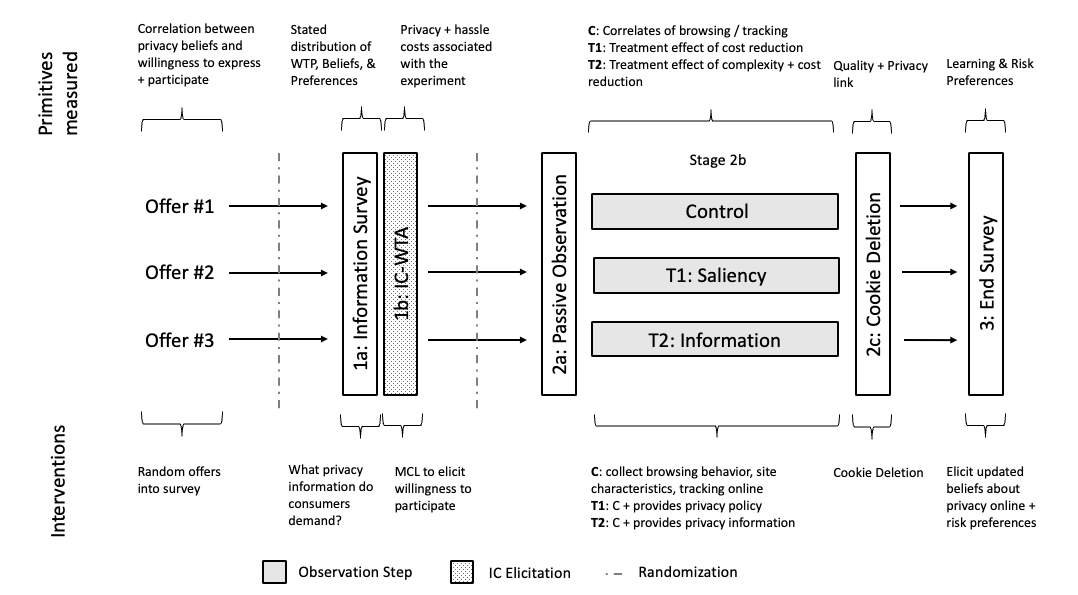
\includegraphics[width=\textwidth]{manual_figures/design/outline_may2025.png}
    \resizebox{\textwidth}{!}{%
    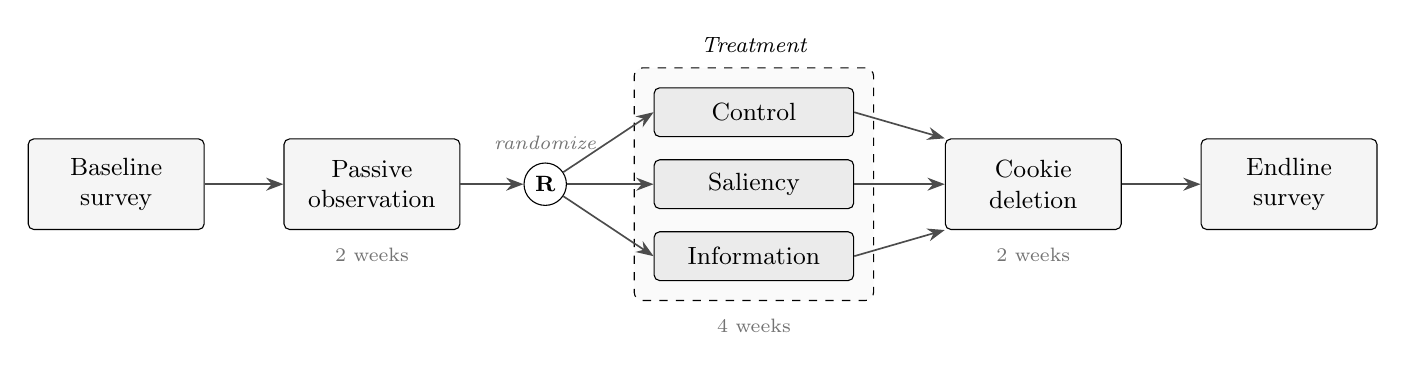
\begin{tikzpicture}[
      font=\small,
      >={Stealth[length=2.2mm]},
      phase/.style={draw, rounded corners=2pt, align=center, minimum height=1.15cm,
                    text width=2.0cm, fill=black!4},
      arm/.style={draw, rounded corners=2pt, align=center, minimum height=0.62cm,
                  text width=2.3cm, fill=black!8},
      arr/.style={->, semithick, draw=black!70},
      dur/.style={font=\scriptsize, text=black!55},
    ]
    \node[phase] (base) {Baseline\\survey};
    \node[phase, right=1.0cm of base] (obs) {Passive\\observation};
    \node[circle, draw, fill=white, right=0.8cm of obs, inner sep=2.2pt,
          font=\footnotesize\bfseries] (rand) {R};
    \node[arm, right=1.1cm of rand] (sal) {Saliency};
    \node[arm, above=0.28cm of sal] (ctrl) {Control};
    \node[arm, below=0.28cm of sal] (info) {Information};
    \node[phase, right=1.15cm of sal] (cookie) {Cookie\\deletion};
    \node[phase, right=1.0cm of cookie] (end) {Endline\\survey};
    \begin{scope}[on background layer]
      \node[draw, dashed, rounded corners=3pt, fit=(ctrl)(info),
            inner sep=7pt, fill=black!2] (trt) {};
    \end{scope}
    \node[above=2pt of trt.north, font=\footnotesize\itshape] {Treatment};
    \draw[arr] (base) -- (obs);
    \draw[arr] (obs) -- (rand);
    \draw[arr] (rand) -- (ctrl.west);
    \draw[arr] (rand) -- (sal.west);
    \draw[arr] (rand) -- (info.west);
    \draw[arr] (ctrl.east) -- (cookie.north west);
    \draw[arr] (sal.east)  -- (cookie.west);
    \draw[arr] (info.east) -- (cookie.south west);
    \draw[arr] (cookie) -- (end);
    \node[dur, below=3pt of obs] {2 weeks};
    \node[dur, below=3pt of trt.south] {4 weeks};
    \node[dur, below=3pt of cookie] {2 weeks};
    \node[font=\scriptsize\itshape, text=black!55, above=1pt of rand] {randomize};
    \end{tikzpicture}%
    }
    \end{center}
    \caption*{\scriptsize \textsc{Notes}: Overview of the study timeline. After a baseline survey eliciting privacy beliefs and conjoint-based privacy preferences, participants' browsing is passively observed for two weeks. They are then randomized into one of three arms for a four-week intervention---\emph{Control} (no privacy information), \emph{Saliency} (privacy policies made salient at lower search cost), or \emph{Information} (simplified, personalized privacy information at lower complexity)---followed by a two-week cookie-deletion phase and an endline survey measuring updated beliefs and risk preferences. Section~\ref{sec:experiment} details each stage, including the screening survey and incentive-compatible willingness-to-accept elicitation.}
\end{figure}

The study begins with a baseline survey that accomplishes four things. First, we replicate a series of questions on privacy practices and attitudes from PEW \citep{PewPrivacy} to assess the representativeness of our sample on privacy attitudes. Second, for each of the 19 privacy attributes in our dataset, we elicit participants' beliefs about their prevalence online. Third, we use a partial-profile conjoint \citep{doi:10.1287/inte.31.3s.56.9676, ALLENBY2019151} to elicit participants' willingness to pay for each privacy practice. Because privacy preferences vary by context, we randomize the website category in which the conjoint is framed.\footnote{See Appendix~\ref{sec:conjoint_details} for additional information on the conjoint.} Fourth, we use a switching multiple-price list \citep{andersen2006elicitation} to incentive-compatibly elicit participants' willingness to accept (WTA) compensation for participating in the observation stage of the study.\footnote{Participants are given an example and complete comprehension questions to ensure they understand the procedure for both the conjoint and the WTA elicitation.}
 
\paragraph{Second stage eligibility.} Following the baseline survey, a random offer from the multiple-price list is chosen for each participant. If their stated WTA is less than or equal to the random offer, they are offered a spot in the second stage and asked to install the browser extension. Eligible participants receive an email containing an installation link and an individualized experiment ID that serves both as validation of successful installation and as a link to our backend-generated identifier, ensuring that we can track each participant across the entire intervention period.\footnote{In the case when the participant has multiple devices, we are able to identify each device individually but the participant across these devices and aggregate across devices for the analysis.}

\subsubsection{Information Intervention \& Treatment Assignment}

Our intervention provides participants with comprehensive and credible information on the privacy practices of the websites they browse. The primary randomization includes a \textit{control}, a \textit{saliency}, and an \textit{information} group. The control group installs the extension, which passively collects time spent, privacy information acquisition, and third-party trackers

\paragraph{Saliency Treatment.} Participants in the saliency group are provided with direct and easy access to website privacy policies. The extension introduces a prominent pop-up in the upper right corner of the browser when a participant arrives on a website. If the participant clicks this link, they are directed to the privacy policy page (see Figure~\ref{fig:saliency_intervention} for an example on the New York Times website). Mapping back to our conceptual framework, this treatment reduces search frictions associated with finding privacy information online but does not change the attention costs associated with comprehension nor the complexity of the information. In the language of our model, this induces experimental variation in $c^s_j$.

\begin{figure}
  \caption{Experimental Intervention}\label{fig:experimental_intervention}
  \centering
  \begin{subfigure}[b]{1.0\linewidth}
    
\includegraphics[width=\linewidth]{manual_figures/dialog/saliency_dialog.png}
    \caption{Saliency Intervention}
    \label{fig:saliency_intervention}
  \end{subfigure}

  \vskip\baselineskip

  \begin{subfigure}[b]{1.0\linewidth}
    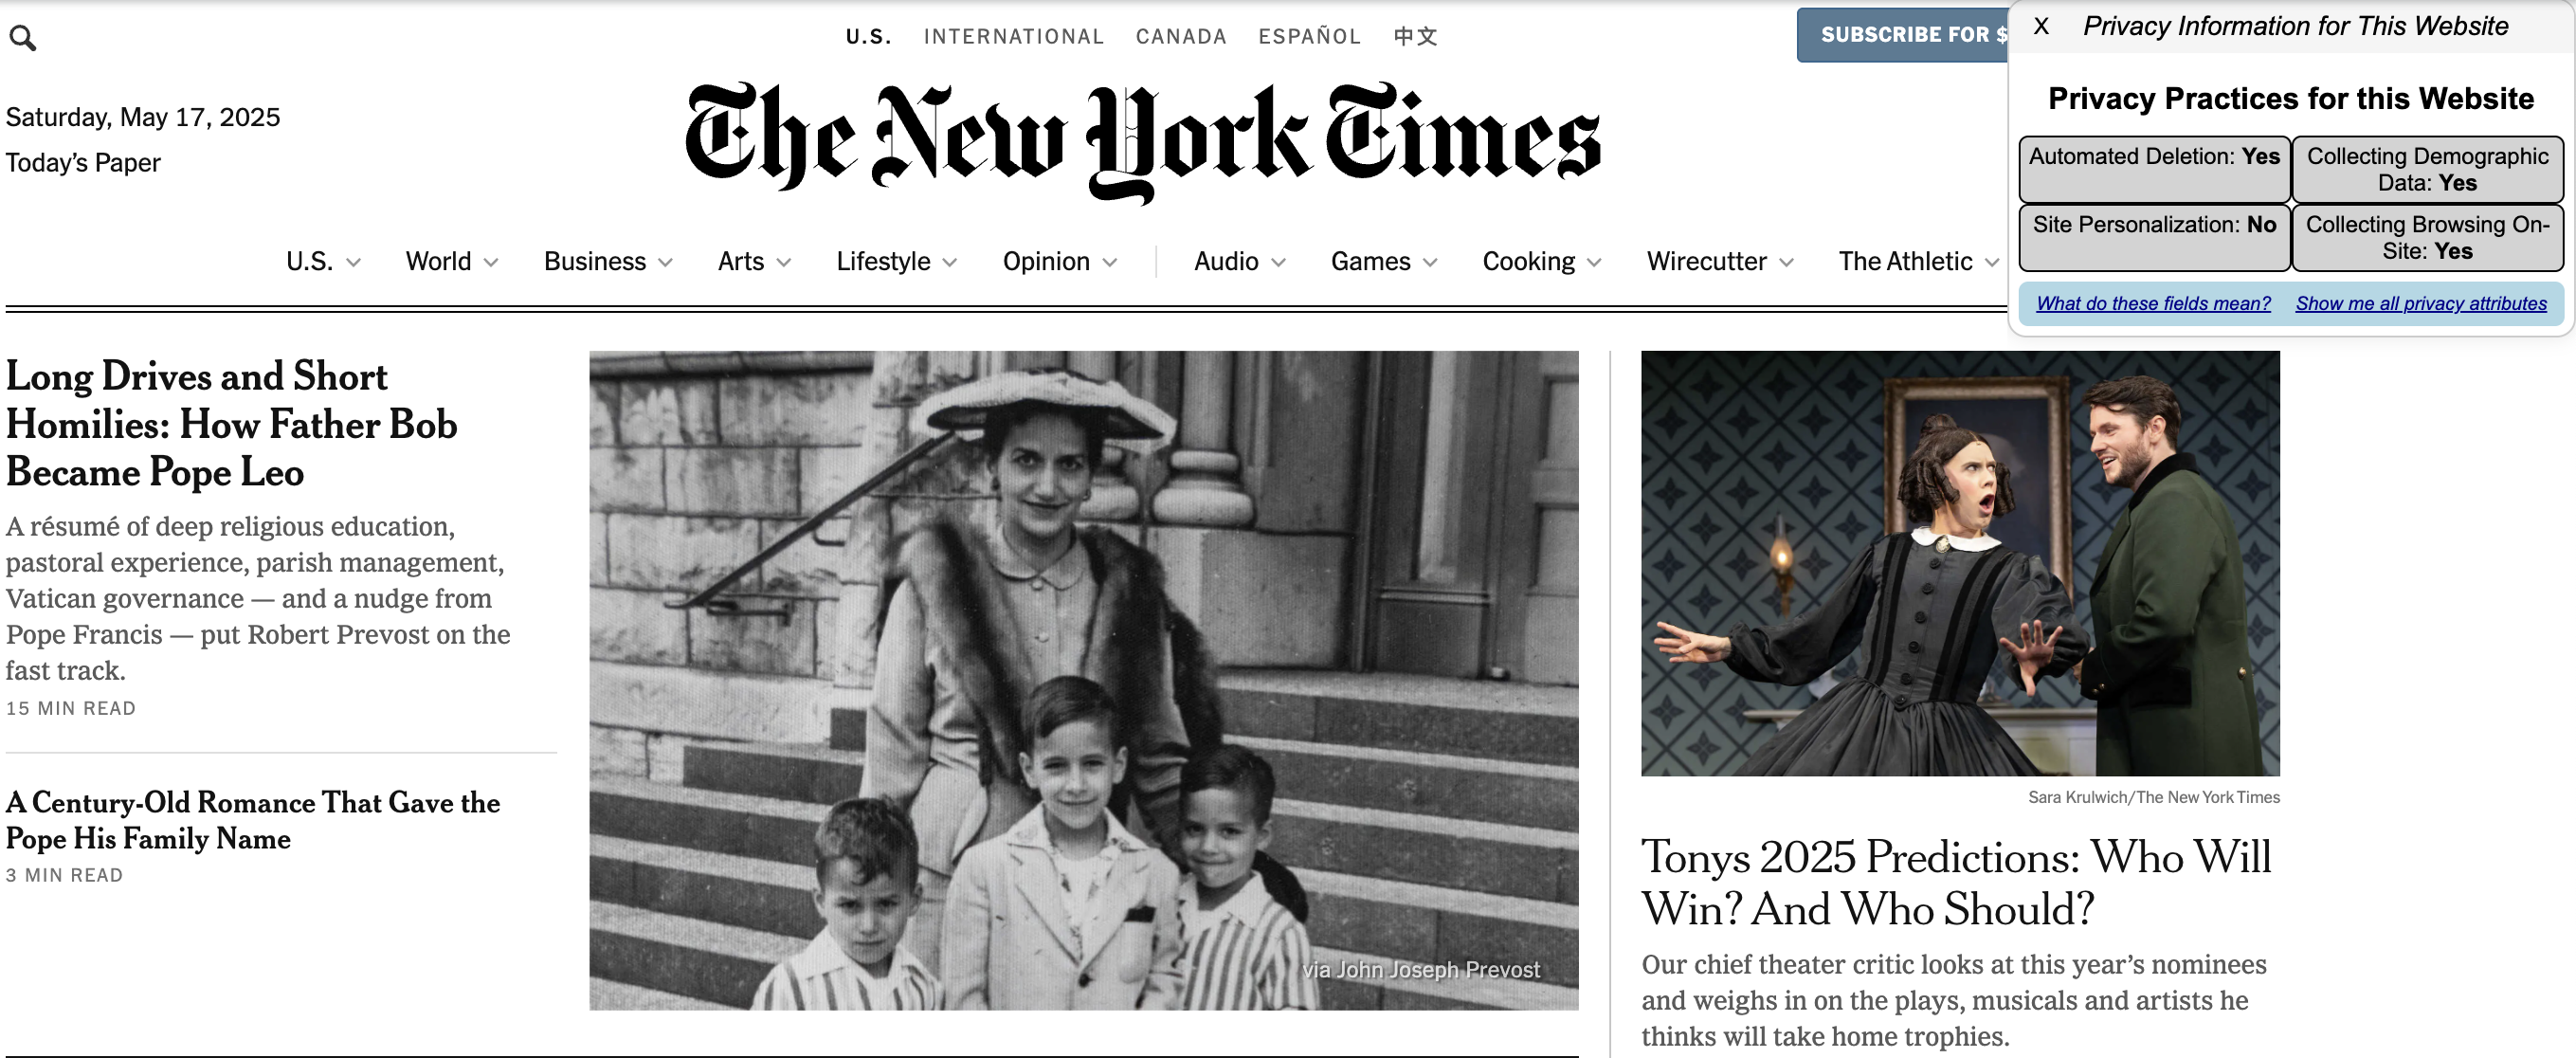
\includegraphics[width=\linewidth]{manual_figures/dialog/info_dialog.png}
    \caption{Information Intervention}
    \label{fig:info_intervention}
  \end{subfigure}
  \label{fig:experimental_interventions}
\end{figure}

\paragraph{Information Treatment.} Participants in the information group are given three pieces of privacy information through a transparent and salient pop-up in the upper right corner of the browser, providing experimental variation in $\alpha_j$ (see Figure~\ref{fig:info_intervention}). Participants can click this box to get additional information on further privacy attributes, as well as definitions of each attribute.\footnote{Participants can click to find extended descriptions of the attributes as well as see the full list of attributes, apart from the three presented. The additional information dialogs can be seen in Figure~\ref{fig:additional_experimental_info}.} 

A key feature of our information treatment is personalization: we select the privacy attributes that are most informative for each individual participant. Two of the three displayed attributes are held constant across websites and personalized using each participant's conjoint estimates and elicited beliefs. Specifically, we calculate the expected information gain from attribute $k$ for individual $i$ as:
\begin{equation}\label{eq:provided_info}
    V_{ik} = E[u_{\text{post}}] - E[u_{\text{prior}}] = \theta^b_{ik}(1 - \theta^b_{ik})\beta_{ik}
\end{equation}
where $\theta^b_{ik}$ is individual $i$'s belief that a random website in the top 500 engages in practice $k$ and $\beta_{ik}$ is their preference weight from the conjoint. The formula captures the intuition that information is most valuable when a participant both cares about the attribute (high $|\beta_{ik}|$) and is uncertain about its prevalence (beliefs near 0.5). We take the two attributes with highest $V_{ik}$ as individual $i$'s personalized treatment. The third attribute is chosen at random and varies across websites.

\subsection{Cookie Deletion State \& Endline}

\paragraph{Third-Party Cookie Deletion.} After four weeks of treatment, we begin the final portion of our intervention, during which we induce exogenous variation in data sharing by randomizing the deletion of third-party advertising and analytics cookies. We identify these cookies using the the custom AdBlockPlus parser built into the Chrome Extension that allows us to identify when a network request is sent to a third-party domain and continually delete these cookies.\footnote{Analysis and categorization of the collected trackers from the extension (using the process described in Appendix \ref{sec:data_collection_appendix}) suggests that these are predominantly third-party domains associated with data collection for advertising and analytics.} Treatment timing is staggered: we randomize within block to have 2  of the 3 participants (for even blocks) or 1 of the 3 participants (for odd blocks) begin cookie deletion at the start of week 7, while the remaining participants start at the beginning of the final week of the study. This staggered rollout generates variation in both the presence and duration of cookie deletion, which we exploit for identification of cookie-value parameters in the structural model (Section~\ref{sec:estimation}).

\paragraph{Endline Survey.} After the treatment period is completed, we conduct an endline survey to validate our treatment. For each participant, we elicit beliefs about the privacy practices of their top 2 preferred attributes on the five most visited websites during the intervention period. In addition, we implement a simple bonus lottery to measure risk preferences \citep{CHARNESS201343, RePEc:kap:jrisku:v:41:y:2010:i:3:p:219-243} and re-elicit privacy attitudes. The full details of questions asked in the surveys is documented in Appendix \ref{sec:survey_appendix}.

\subsection{Experimental Implementation and Sample}

\paragraph{Timeline and Recruitment.}  We conducted our experiment from June 14th until August 23rd, 2025, recruiting participants based in the United States from both CloudResearch Connect and Prolific. Recruitment occurred in two waves, with the first wave running from June 14th until August 9th and the second from June 28th until August 23rd. Participants recruited in each wave followed the same timeline conditional on study start date. 

\begin{figure}[H]
\caption{Participant Flow through Study}
\label{fig:subject_flow}
\begin{center}
% Previous flow diagram kept for reference:
% 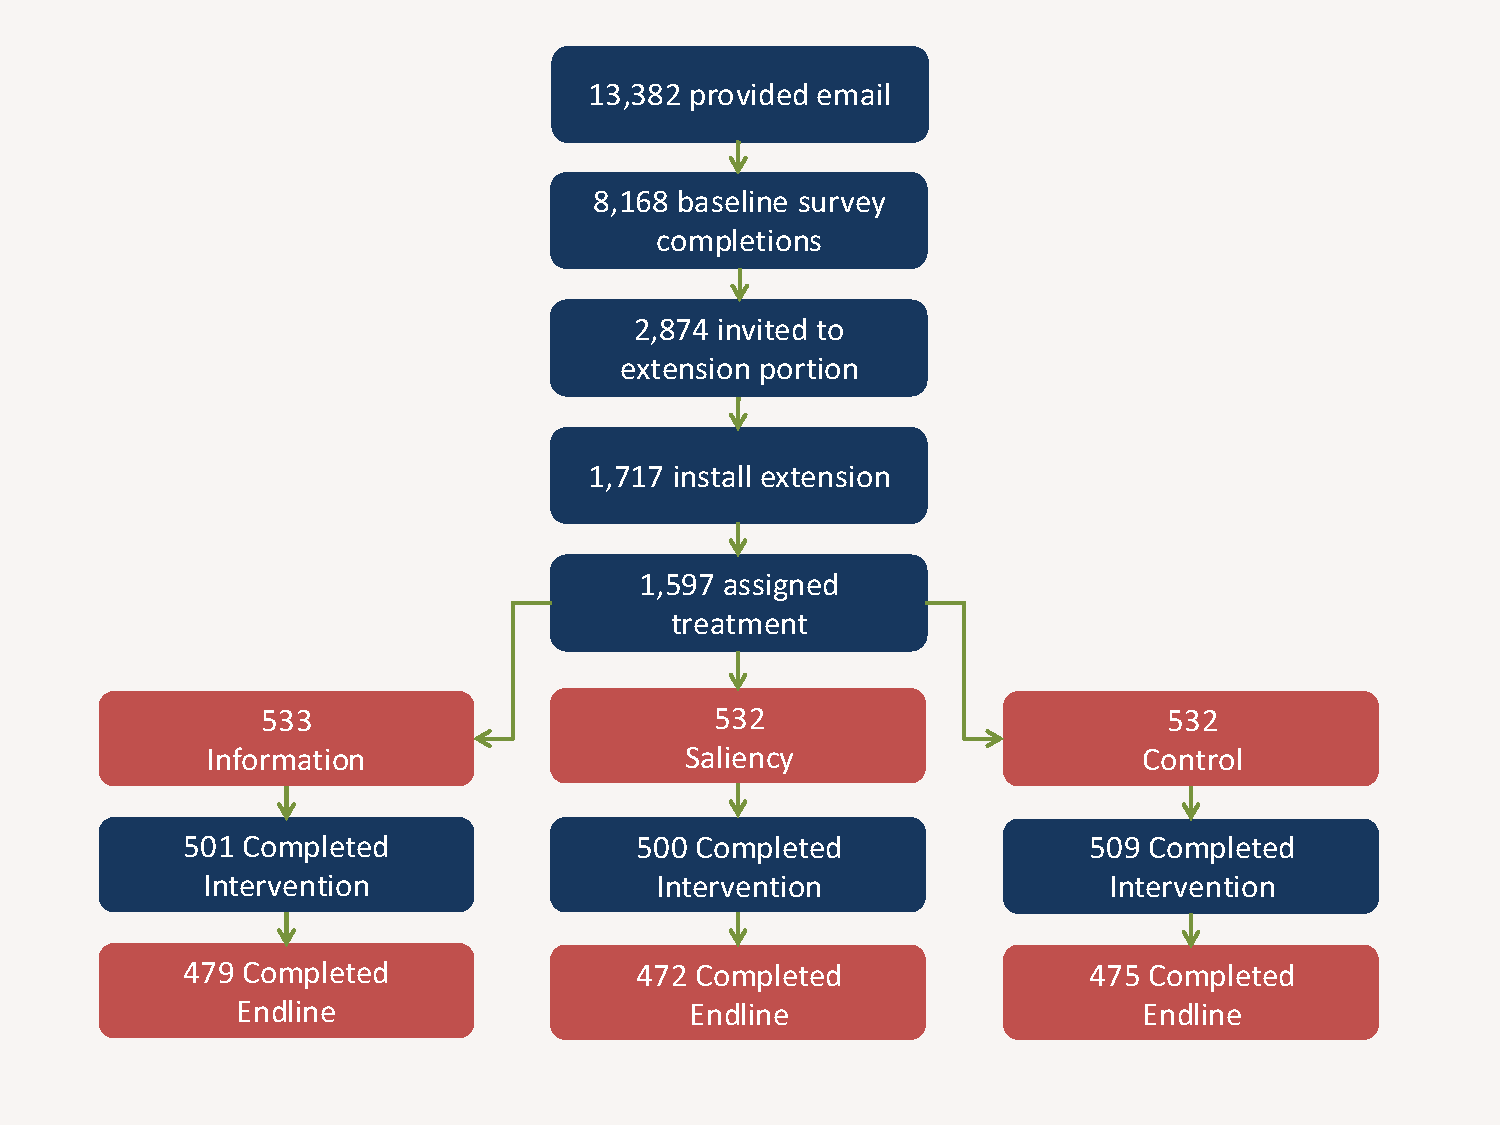
\includegraphics[scale=0.5]{manual_figures/design/subject_flow.pdf}
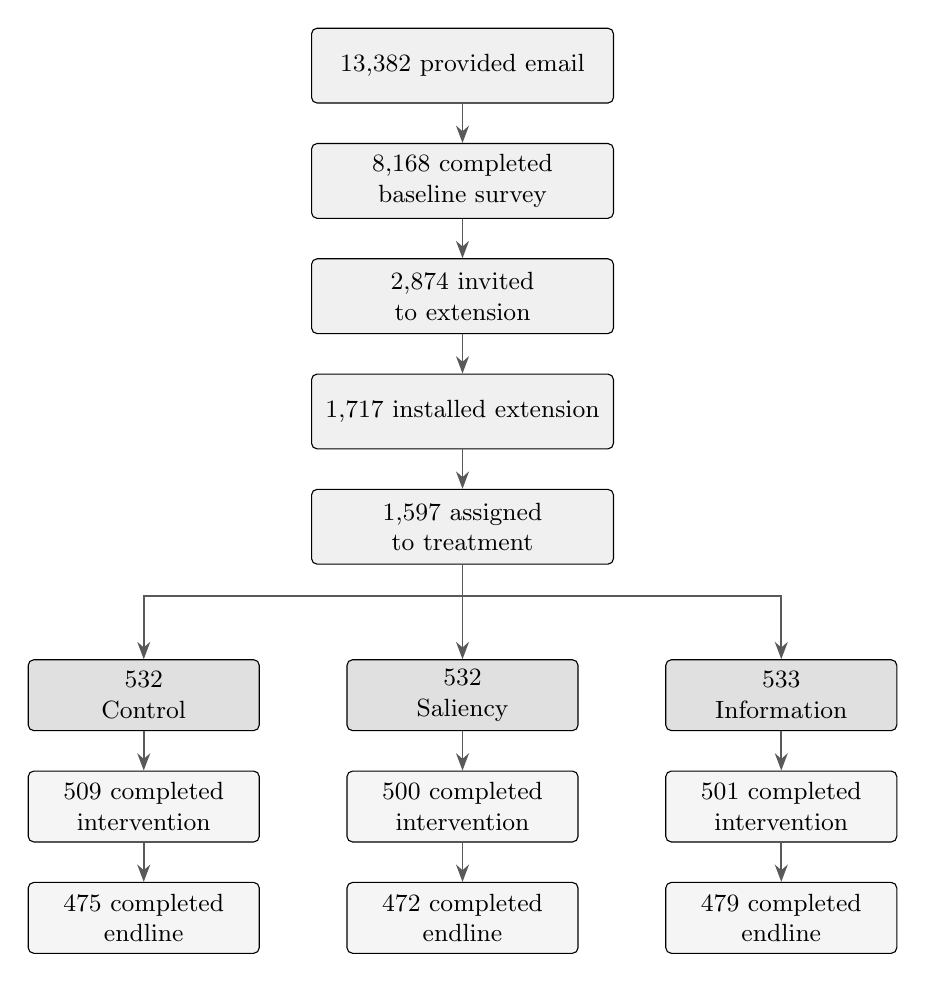
\begin{tikzpicture}[
  font=\small,
  >={Stealth[length=2.2mm]},
  fbox/.style={draw, rounded corners=2pt, align=center, text width=3.6cm,
               minimum height=0.95cm, fill=black!6},
  abox/.style={draw, rounded corners=2pt, align=center, text width=2.7cm,
               minimum height=0.9cm, fill=black!4},
  ahead/.style={draw, rounded corners=2pt, align=center, text width=2.7cm,
                minimum height=0.9cm, fill=black!12},
  arr/.style={->, semithick, draw=black!65},
  node distance=0.5cm,
]
\node[fbox] (f1) {13,382 provided email};
\node[fbox, below=of f1] (f2) {8,168 completed baseline survey};
\node[fbox, below=of f2] (f3) {2,874 invited to extension};
\node[fbox, below=of f3] (f4) {1,717 installed extension};
\node[fbox, below=of f4] (f5) {1,597 assigned to treatment};
\draw[arr] (f1)--(f2);
\draw[arr] (f2)--(f3);
\draw[arr] (f3)--(f4);
\draw[arr] (f4)--(f5);
\node[ahead, below=1.2cm of f5] (sal1)  {532\\Saliency};
\node[ahead, left=1.1cm of sal1] (ctrl1) {532\\Control};
\node[ahead, right=1.1cm of sal1] (info1) {533\\Information};
\node[abox, below=of ctrl1] (ctrl2) {509 completed\\intervention};
\node[abox, below=of sal1]  (sal2)  {500 completed\\intervention};
\node[abox, below=of info1] (info2) {501 completed\\intervention};
\node[abox, below=of ctrl2] (ctrl3) {475 completed\\endline};
\node[abox, below=of sal2]  (sal3)  {472 completed\\endline};
\node[abox, below=of info2] (info3) {479 completed\\endline};
\draw[arr] (f5.south) -- (sal1.north);
\draw[arr] (f5.south) -- ++(0,-0.4) -| (ctrl1.north);
\draw[arr] (f5.south) -- ++(0,-0.4) -| (info1.north);
\draw[arr] (ctrl1)--(ctrl2); \draw[arr] (ctrl2)--(ctrl3);
\draw[arr] (sal1)--(sal2);   \draw[arr] (sal2)--(sal3);
\draw[arr] (info1)--(info2); \draw[arr] (info2)--(info3);
\end{tikzpicture}
\end{center}
\end{figure}

Figure \ref{fig:subject_flow} presents the flow of participants through the study. Of the \fullCohortN{} participants who provided their email and use Google Chrome, \baselineSurveyN{} (\baselineCompletionPct{}\%) completed the baseline survey. Of these, \eligibleN{} were eligible for the extension phase (\eligiblePct{}\%), \installedN{} successfully installed the extension (\installedPctOfEligible{}\% of eligible), and \remainedN{} remained by the time treatment was assigned (\remainedPct{}\%). The drop from \installedN{} to \remainedN{} is attributable to technical issues with older laptops, manual removal of participants with abnormal behavior, and general attrition. Throughout, we refer to the participants who completed the baseline survey as the \textit{survey} sample and those who completed the extension portion of the study as the \textit{extension} sample. For the extension sample, the study proceeds as follows:
\begin{enumerate}
\item Baseline Period (two weeks)
\item Primary Information Intervention Period (four weeks)
\item Cookie deletion (two weeks)
\begin{itemize}
    \item First wave of third-party cookie deletion (two weeks)
    \item Second wave of third-party cookie deletion (one week)
\end{itemize}
\item Endline Survey (one day after extension uninstall)
\end{enumerate}

\paragraph{Experimental Sample.} The average participant in the survey sample is \surveyMeanAge{} years old, \surveyFemalePct{}\% of the sample is female, and \surveyCollegePct{}\% of the sample has at least a college education. To assess demographic representativeness, we compare the demographic composition to the 2021 U.S. Census on age, education, gender, and income in Figure \ref{fig:dem_balance}. Overall, our sample is reasonably representative but skews younger, more female, and more educated than a fully representative sample. Importantly, the demographic composition is consistent between the survey and extension samples.

In the baseline period, the average participant spends \baselineDailyHoursPrivacy{} hours on websites with privacy information and \baselineDailyHoursLeisure{} hours online.\footnote{Since our participants are recruited from survey recruiting platforms, for this calculation and throughout the paper, we drop time spent on survey websites (e.g., qualtrics, surveymonkey) and recruitment platforms (e.g., prolific, cloudresearch, mturk, paidviewpoint). This ensures that we are focusing on `leisure' sites as opposed to `labor' sites. Including usage on these websites increases the average daily time spent online to \baselineDailyHoursAll{} hours.} The top websites used by participants are displayed in Table \ref{tab:top_websites} and correspond to domains consistent with the top most visited domains for which we collect privacy information -- e.g., YouTube, Google,  Facebook.

To ensure similar exposure to the information intervention across treatment groups, we block-randomize based on baseline usage. Specifically, we order participants by their total time spent on websites for which privacy information is available and, within each consecutive block of three participants, randomly assign treatments. In addition, we enforce balance on total time spent, demographics, privacy knowledge, WTA, beliefs, and conjoint category. Table~\ref{tab:exp_balance_table} confirms that this procedure achieves balance across treatment groups on each of these dimensions.

From the experimental sample, \extensionInfoFinalN{} (of \extensionInfoStartN{}), \extensionSaliencyFinalN{} (of \extensionSaliencyStartN{}), and \extensionControlFinalN{} (of \extensionControlStartN{}) participants remained in the information, saliency, and control groups, respectively, with their extensions installed at the end of the intervention.\footnote{When participants uninstall the extension, they are automatically opted out of the study.} Of these, \surveyEndlineInfoN{}, \surveyEndlineSaliencyN{}, and \surveyEndlineControlN{} completed the endline survey.\footnote{Some of the attrition between the final extension sample and the endline survey is driven by email delivery issues.} Standard balance checks provide no statistical evidence of differential attrition: chi-square tests across treatment groups yield $p = \attritionExtensionPvalue{}$ for the extension sample and $p = \attritionEndlinePvalue{}$ for the endline sample, and logistic regressions with attrition as the dependent variable confirm the absence of overall or pairwise differential attrition \citep{gerber2012field}.

\subsection{Selection into Study Based on Privacy Preferences}\label{sec:selection}

A key concern with our study is that we are studying privacy preferences using data collection that is potentially privacy-invasive. Our study is designed to precisely measure the magnitude of this selection. There are three points at which selection on privacy preferences might occur: into the recruiting platforms, into responding to the survey, and into installing the Chrome Extension. We address each in turn and find no evidence of meaningful selection on privacy preferences at the first two stages; at the third stage, our WTA measure allows us to precisely bound the extent of selection.

\paragraph{Selection into the survey.} We mitigate possible selection by advertising the study generically, with no mention of privacy. To characterize any remaining selection, we randomize the advertised first-stage survey payments between \$3, \$4, and \$5. If privacy preferences influence the decision to participate, we would expect our measured privacy preferences and belief misspecification to monotonically vary with the survey payments. Figure~\ref{fig:selection_on_survey_payments} compares aggregated belief error measures, our PEW index, and WTA across the different survey payments and reveals little systematic variation.

\paragraph{Selection into the platform.} Online recruitment platforms may suffer from selection bias, as their users are likely more willing to share information online than the general population. To quantify this, we replicate a subset of questions from PEW's nationally representative survey on privacy preferences. Figure~\ref{fig:pew_comparison} compares our results with PEW's. On average, our participants are more likely to immediately accept privacy policy terms and more likely to switch websites due to privacy, with similar beliefs about policy effectiveness. Given there is no clear ordering between the samples in terms of privacy sensitivity, we interpret this as indicating that platform-level selection based on privacy preferences is not dramatic.

\paragraph{Selection into the extension.} While the survey is advertised generically, the purpose of the experiment becomes clearer once participants are asked to install a browser extension that continuously monitors their browsing. We expect more privacy-sensitive participants to require higher compensation. The final part of the survey uses the incentive-compatible WTA mechanism to directly measure this. The median (mean) WTA in the invited sample is \$\wtaInvitedMedian{} (\$\wtaInvitedMean{}), compared to \$\wtaFullMedian{} (\$\wtaFullMean{}) in the full survey population. Differences arise from a cap on maximum compensation of \$40, which we impose to manage experimental costs. Interpreting WTA as a proxy for privacy preferences, our final experimental sample allows us to estimate treatment effects for the bottom \invitedSampleCoveragePct{}\% of participants in terms of the intensity of privacy preferences. Our estimates are informative about the large majority of the population but may not generalize to the most privacy-sensitive individuals. Figure \ref{fig:extension_survey_conjoint_sample} compares the conjoint estimates between the full survey sample and the extension sample finding that, while the privacy valuations for the survey sample are higher for most attributes, the relative ordering is the same and the difference is not dramatic.

\section{Privacy Practices, Beliefs, and Stated Preferences }\label{sec:privacy_practices_online}

For our information intervention to influence participant choices, three conditions must hold: there must be meaningful heterogeneity in privacy practices across websites within plausible substitute sites, participants must have uncertainty about the privacy practices of sites, and the attributes on which we provide information must be ones participants care about. In this section, we document that all three conditions are satisfied.

\begin{figure}[ht]
\caption{Privacy Practices across Website Categories}\label{fig:scores_by_category}
\begin{center}
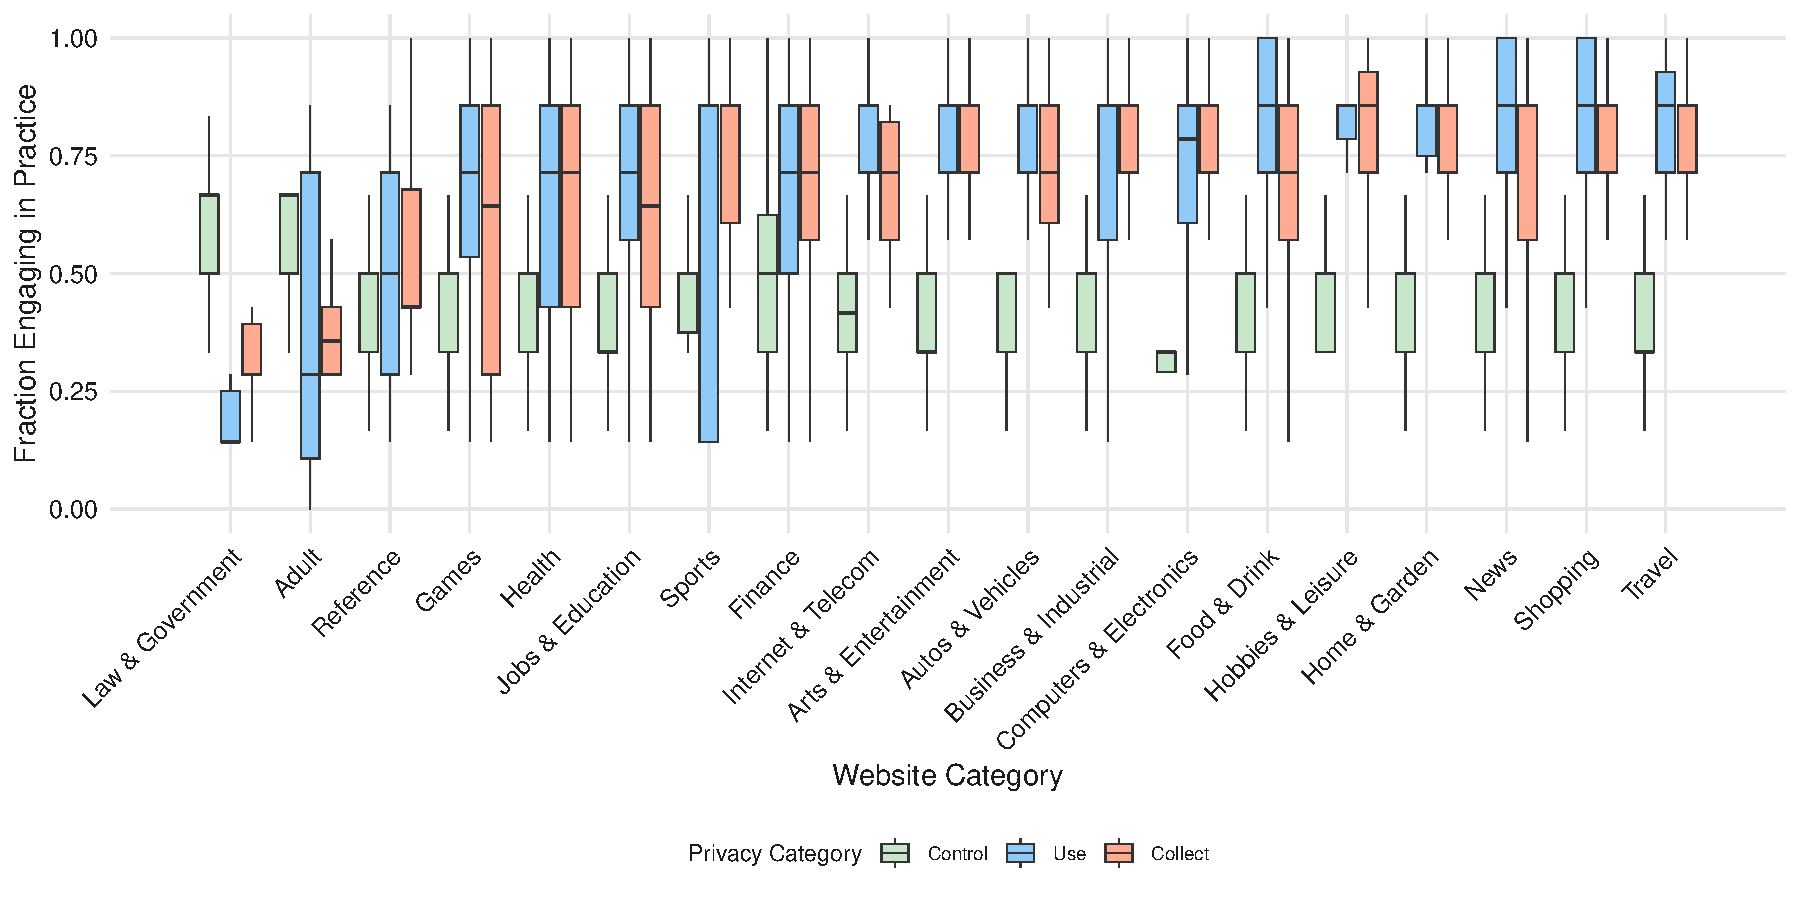
\includegraphics[scale=.5]{./output/figures/domain_scores_box_plot.pdf}
\end{center}
\caption*{\scriptsize \textsc{Notes}:  Distribution of privacy practice counts by website category. Privacy practices hand-coded from privacy policies of top 500 US websites and aggregated into three indices: collect (8 attributes), control (5 attributes), and use (7 attributes). Each website receives a score equal to the count of practices engaged in within each category. Website categories obtained from the Klazify API. Box plots display median, interquartile range, and outliers.}
\end{figure}

\subsection{Privacy Practice Heterogeneity}
We begin by characterizing variation in privacy practices across websites. We categorize each website using the Klazify API and aggregate each domain into a single score for each of the three privacy practice categories described in Table~\ref{tab:characteristics}: \emph{collect} (8 attributes relating to data collection), \emph{use} (7 attributes relating to how data is shared), and \emph{control} (5 attributes relating to user protections). Based on our conjoint estimates (discussed below), engaging in more ``control'' practices is generally utility-improving for participants, while engaging in more ``collect'' or ``use'' practices is utility-decreasing.


Figure~\ref{fig:scores_by_category} presents box plots documenting the variation in these indices across website categories. Two patterns stand out. First, there is considerable heterogeneity \emph{within} categories --- even among websites offering similar content, privacy practices vary substantially. This is precisely the variation that informed participants could act on. Second, while median scores are relatively similar across categories, two notable exceptions emerge: ``Law \& Government'' and ``Adult.'' These categories consist of websites that naturally collect more sensitive information (e.g., legal records, health data), and accordingly tend to have stricter privacy practices. This pattern provides useful validation that our hand-coded data captures meaningful differences.

\begin{figure}[ht]
    \centering
    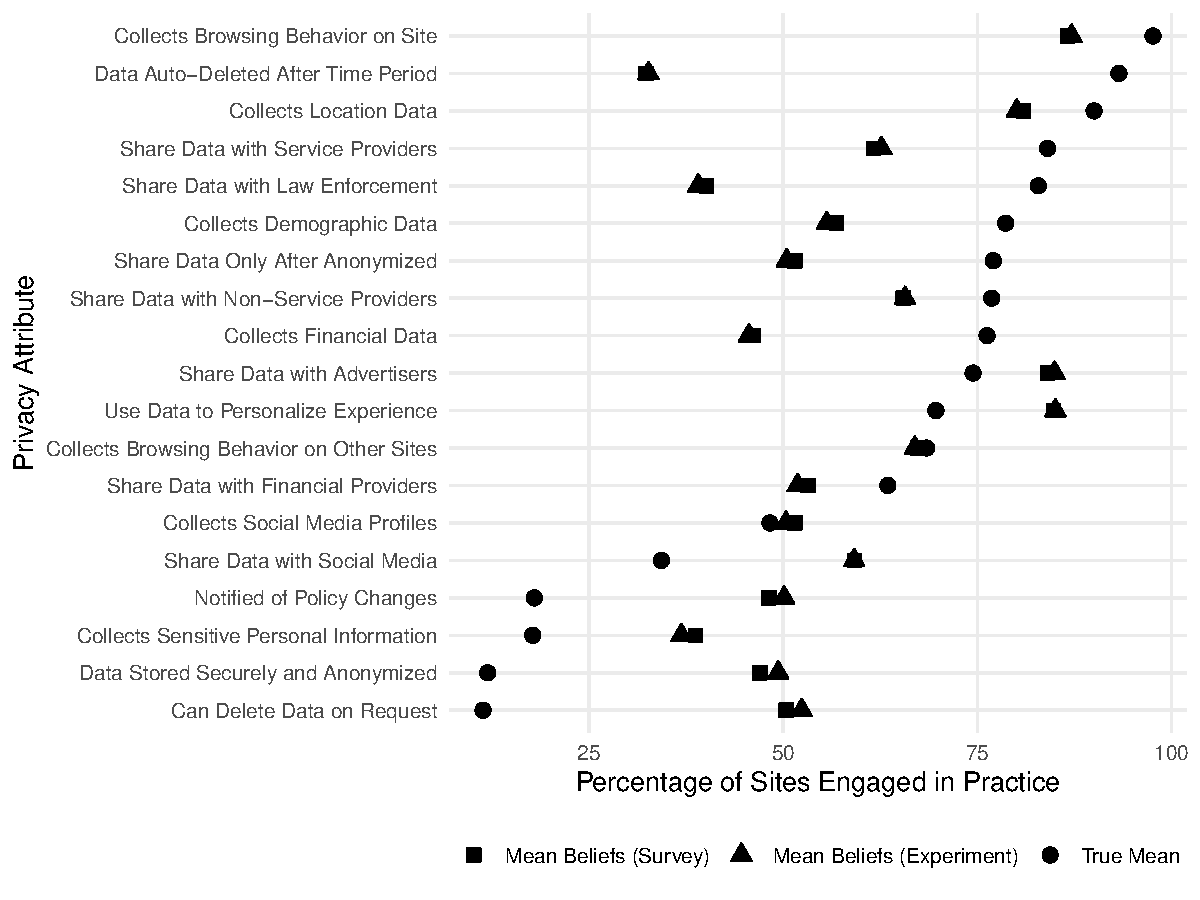
\includegraphics[scale=.5]{./output/figures/beliefs_vs_truth.pdf}
    \caption{Aggregate Beliefs about Privacy Practices}
    \label{fig:privacy_info_beliefs}
    \caption*{\scriptsize \textsc{Notes}: Mean prior beliefs versus ground truth prevalence. Beliefs elicited on 5-point Likert scale, converted to percentage points via the transformation $(r - 1) \times 25$, where $r \in \{1,2,3,4,5\}$. Ground truth computed as the proportion of websites engaging in each practice. }
\end{figure}

\subsection{Beliefs about Privacy Practices}

We next characterize what participants believe about privacy practices and how these beliefs compare to our collected data. In the baseline survey, we ask each participant: ``For a random website in the top 500 online, how likely do you think it is they engage in [PRIVACY PRACTICE]?'' for each of the 19 attributes.

Figure~\ref{fig:privacy_info_beliefs} presents mean beliefs alongside the true prevalence of each attribute.\footnote{Figure~\ref{fig:privacy_info_beliefs} displays beliefs for both the extension and survey sample showing that the selection into the experiment does not induce large differences in participants' beliefs about the prevalence of privacy practices online.} Participants' beliefs are clearly misspecified for most attributes, though the direction of misspecification varies. For instance, participants correctly perceive that on-site browsing behavior and location data are among the most commonly collected attributes, but they underestimate the extent of this collection. Conversely, participants substantially overestimate the prevalence of data collection for advertising purposes --- consistent with public discourse around online privacy focusing disproportionately on advertising. Column (1) of Table \ref{tab:baseline_demo_heterogeneity} shows that the only significant demographic predictor of misspecification is education as individuals with a bachelor's degree or above have a lower degree of misspecification.

\begin{figure}[ht]
\centering
\caption{Willingness to Pay for Privacy Attributes}
\label{fig:privacy_combined}\label{fig:privacy_info_partworth}
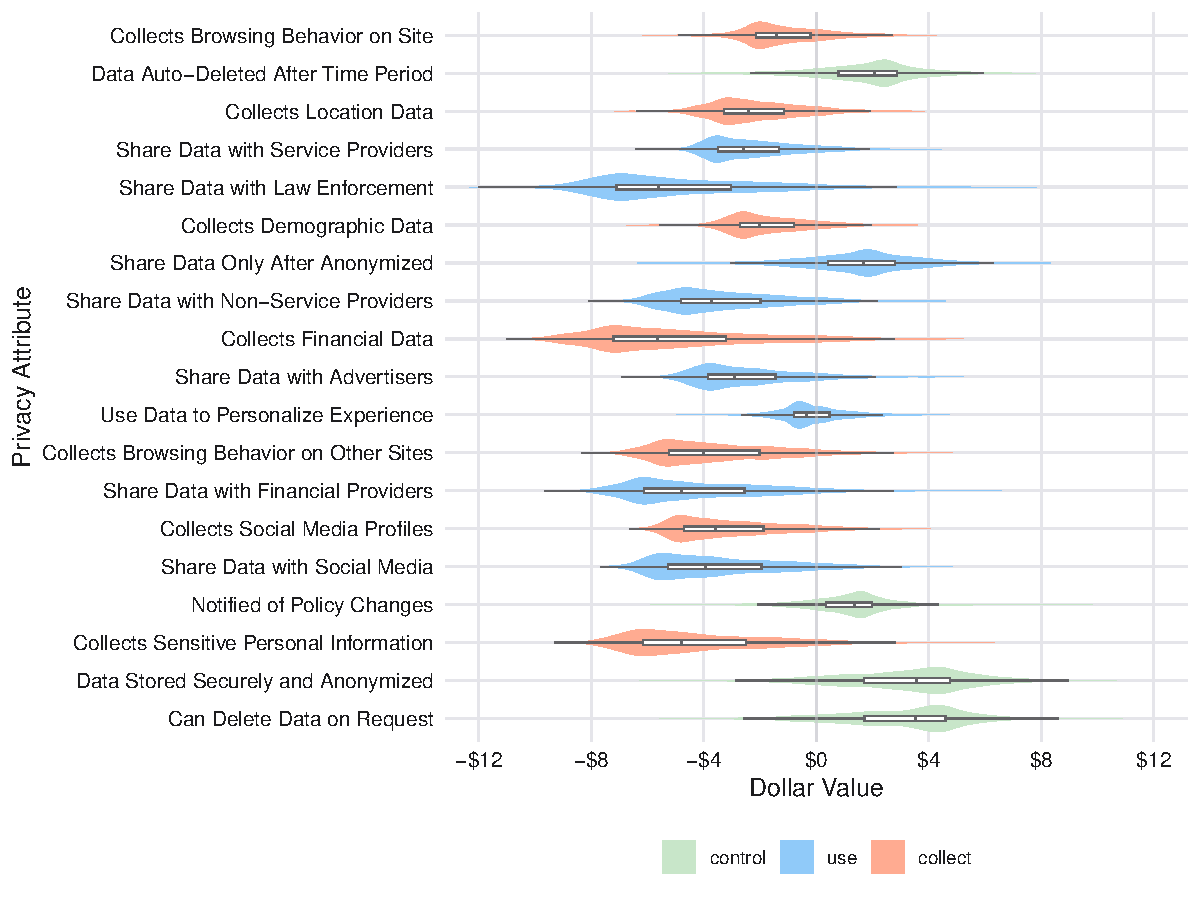
\includegraphics[width=0.62\textwidth]{./output/figures/individual_heterogeneity_dollars_with_website_extension.pdf}
\vspace{0.4em}
\caption*{\scriptsize \textsc{Notes}: Estimated monthly willingness to pay for different privacy attributes among the extension sample of participants who installed the browser extension, computed using the estimated part-worth for each attribute and the price coefficient. Green rows denote ``Control'' attributes, blue rows denote ``Use'' attributes, and orange rows denote ``Collect'' attributes. Appendix \ref{sec:conjoint_details} contains the estimation details; the full conjoint sample version is in Figure \ref{fig:privacy_combined_full}.}
\end{figure}

\subsection{Stated Privacy Preferences}\label{subsec:stated_privacy_prefs}

To understand which privacy attributes participants value most, we estimate willingness to pay (WTP) for each attribute from the conjoint task completed in the baseline survey. Figure~\ref{fig:privacy_info_partworth} presents the estimated monthly WTP.\footnote{We derive WTP by dividing the estimated part-worth for each attribute by the price coefficient. Appendix~\ref{sec:conjoint_details} contains the full estimation details.} Control attributes --- data deletion, data security, anonymization --- are associated with positive WTP, consistent with participants viewing these protections as valuable. In contrast, collect and use attributes are associated with negative WTP: participants would need to be compensated for using a website that collects financial data, shares information with law enforcement, or collects sensitive personal information. Column (2) of Table \ref{tab:baseline_demo_heterogeneity} shows that education, being over 60, and being female are associated with valuing privacy more highly.\footnote{Reassuringly, preferring not to answer the question on gender is associated with the largest predicted increase in privacy preference intensity.}

The most valued attributes are those associated with potential off-platform consequences: collecting (\$\wtpCollectFinancial{}/month) and sharing (\$\wtpShareFinancial{}/month) financial information, sharing with law enforcement, collecting sensitive information, and data security. This pattern is consistent with participants' self-reported concerns about data sharing (Table~\ref{tab:data_sharing_purpose}), which emphasize loss of data control, identity theft, and hacking as the most important consequences.\footnote{\cite{bian2023consumer} document that Apple's App Tracking Transparency allowed consumers to meaningful reduce these harms through changing their data sharing practices -- indicating that information on privacy practices could help consumers take action to reduce the likelihood of these consequences.}

\subsection{Distribution of Personalized Treatment Attributes}

The personalized attributes provided to each participant in the information treatment reflect the combination of these two inputs --- preferences and belief uncertainty --- through Equation~\eqref{eq:provided_info}. Attributes appear in a participant's personalized set when the participant both cares about the attribute and believes there is meaningful variation in practices across websites.

Figure~\ref{fig:privacy_info_top_2} presents the distribution of the top 2 personalized attributes across participants. Collecting and sharing financial data, sharing data with law enforcement, data security, data deletion, and collecting sensitive information are the most prominent. Conversely, attributes that participants believe are nearly universal (such as collecting location or on-site browsing data) or that they do not value highly rarely appear in the personalized set. This distribution characterizes the attributes for which our estimated treatment effects reflect the impact of providing information. An important implication is that we provide each participant with information on the attributes they are most likely to act on. 

Finally, we examine the cross-sectional relationship between consumers' belief accuracy about privacy practices and their preference intensity from the conjoint experiment.\footnote{Part-worths are converted so that positive values uniformly indicate disutility from the practice.} Table \ref{tab:conjoint_vs_beliefs} reports the results.  Column (1) shows that respondents who underestimate the prevalence of a practice have \misspecUnderPartworth{} higher part-worths than the correctly informed (\misspecUnderSD{} SD of the part-worth distribution). Column (2) confirms that overestimating prevalence is associated with lower part-worths: a one standard deviation increase in misspecification corresponds to a \misspecLinearSD{} SD decrease in preference intensity. Column (3) shows this is driven entirely by underestimation -- those who overestimate prevalence are no different from the correctly informed. In other words, the consumers who would penalize invasive practices most in their choices are precisely those who are unaware of how common those practices are.

\section{Information Acquisition and Beliefs}\label{sec:hyp_info_beliefs}

This section evaluates Hypotheses 1 and 2 --- whether and to what extent participants in the intervention engaged in information acquisition and changed their knowledge of privacy practices. The results reveal a sharp asymmetry: reducing search costs dramatically increases search behavior but produces no improvement in knowledge, whereas reducing information complexity leads to meaningful learning. We document this in two steps, first examining beliefs directly (Section~\ref{sec:knowledge_top_sites}) and then decomposing the underlying search and learning mechanisms (Section~\ref{sec:search_learning}).
 
\subsection{Beliefs and Knowledge of Privacy Practices for Most Frequented Sites}\label{sec:knowledge_top_sites}

If participants attended to and internalized the information provided during the experiment, they would be most knowledgeable about the privacy practices of the sites they visit most often and the attributes they care most about. Accordingly, we personalize the endline survey to elicit beliefs for each participant's top two preferred attributes on their five most visited sites during the intervention period. We then compare belief accuracy across treatment conditions using the following regression:
$$|\theta^b_{ijk} - \mu^*_{jk}| = \beta T_i + \eta_j + \eta_b + \epsilon_{ijk}$$
where $\eta_b$ represents fixed effects for the experimental block and $\eta_j$ represents fixed effects for the website. The dependent variable measures the absolute distance between the participant's self-reported likelihood that website $j$ engages in practice $k$ and the truth (which is 0 or 100 by construction). We also consider binarized measures of correctness: a weak measure that excludes neutral responses of 50, and a strict measure that classifies a participant as correct if their belief exceeds 50 when (and only when) the website engages in the practice. The continuous measure captures the magnitude of misspecification; the binary measures capture whether participants get the direction right.

\begin{table}[ht]
   \caption{Belief Correctness on Top Sites -- Provided Information}\label{tab:belief_correctness_top_sites}
   \centering
   \scalebox{0.8}{
   
\begin{table}[htbp]
   \caption{Belief Correctness on Top Sites -- Provided Information}
   \centering
   \begin{tabular}{lccc}
      \tabularnewline \midrule \midrule
                            & $\lvert \text{Belief} - \text{Truth} \rvert$     & Correctness (Weak) & Correctness (Strict) \\   
      Model:                & (1)                                              & (2)                & (3)\\  
      \midrule
      \emph{Variables}\\
      Saliency Treatment    & -0.230                                           & -0.006             & 0.004\\   
                            & (0.872)                                          & (0.015)            & (0.013)\\   
      Information Treatment & -5.89$^{***}$                                    & 0.083$^{***}$      & 0.081$^{***}$\\   
                            & (0.867)                                          & (0.014)            & (0.012)\\   
      \midrule
      \emph{Fixed-effects}\\
      Website FE            & Yes                                              & Yes                & Yes\\  
      Block FE              & Yes                                              & Yes                & Yes\\  
      \midrule
      \emph{Fit statistics}\\
      Observations          & 11,727                                           & 9,182              & 11,727\\  
      R$^2$                 & 0.13416                                          & 0.15636            & 0.12222\\  
      Within R$^2$          & 0.00600                                          & 0.00645            & 0.00539\\  
      \midrule \midrule
      \multicolumn{4}{l}{\emph{Clustered (experiment\_id) standard-errors in parentheses}}\\
      \multicolumn{4}{l}{\emph{Signif. Codes: ***: 0.01, **: 0.05, *: 0.1}}\\
   \end{tabular}
\end{table}



   }
   \caption*{\scriptsize \textsc{Notes}:  OLS estimates from Equation (3). Includes website and randomization block fixed effects. Column (1): Dependent variable is $|\text{Belief}_{ijk} - \text{Truth}_{jk}|$, where beliefs are scaled to $\{0, 25, 50, 75, 100\}$ and truth is binary $\{0, 100\}$. Column (2): Binary indicator equal to 1 if response is correct, excluding neutral responses of 50. Column (3): Strict correctness, equal to 1 if $(\text{Belief} > 50) = (\text{Truth} = 100)$. The beliefs are the likelihood of the website engaging in the specified privacy practice for the top 5 most visited sites during the intervention and for the top 2 most informative attributes according to Equation \eqref{eq:provided_info}.}
\end{table}

Table~\ref{tab:belief_correctness_top_sites} presents the results. The information treatment produces a clear improvement in belief accuracy across all specifications. Column (1) indicates that participants in the information group are \beliefDistanceInfoPP{} percentage points closer to the true privacy practices than those in the control group. To put this in context, the median participant in both the control and saliency groups has a belief error of \beliefErrorMedianBaseline{} --- indicating that even for their most visited websites and most valued attributes, participants are essentially at the midpoint of the scale. Against this baseline, a \beliefDistanceInfoPP{} pp improvement represents a meaningful shift, though substantial misspecification remains. Columns (2) and (3) use the binarized correctness measures and show that information group participants are \beliefCorrectStrictInfoPP{}--\beliefCorrectWeakInfoPP{} percentage points more likely to correctly identify a site's privacy practices.

Equally striking is the null result for the saliency group: the point estimates are close to zero and, if anything, slightly negative. Making privacy policies dramatically easier to find --- as we show below, the saliency treatment increases privacy policy visits by a factor of \policyVisitSaliencyFold{} --- produces no detectable improvement in knowledge about privacy practices. This result has direct implications for disclosure policy: regulatory approaches that focus on making privacy policies more accessible, without also reducing their complexity, are unlikely to meaningfully inform consumers.
 
We probe the robustness of these results along two dimensions. First, Table~\ref{tab:belief_correctness_top_sitesrandom_info} estimates the same specification for a random attribute not in the participant's top two personalized attributes. While directionally consistent --- the information group shows a statistically significant improvement relative to the control group --- the estimated effect size is substantially smaller. This suggests that participants primarily internalize the highlighted information from the popup rather than seeking out additional details, but their exposure to the random information also weakly shifted their beliefs. Second, we evaluate the CDF of belief errors across treatment groups (Figure~\ref{fig:cdf_belief_correctness_top_sites}). The distributions for the saliency and control groups are nearly identical, while the information group produces a visibly left-shifted and steeper CDF, implying both higher average accuracy and lower within-group dispersion.

A natural question is whether more time spent on a website leads to better knowledge of its privacy practices. We partition (website, participant) tuples within each experimental group into terciles based on baseline visit frequency and plot mean belief correctness across conditions and terciles (Figure~\ref{fig:top_sites_heterogeneity_exposure}). Two patterns emerge. First, within the control and saliency groups, there is little variation across terciles --- even heavy users of a website know little about its privacy practices. Second, participants in every exposure tercile of the information group are significantly more accurate than participants in any tercile of the other groups. Within the information group, accuracy increases modestly with exposure, but this within-condition gradient is small relative to the overall treatment effect. The dominant source of variation is between treatments, not within them.

\subsection{Quantifying Search and Learning}\label{sec:search_learning}

The preceding results establish \emph{what} happened: the information group learned about privacy practices while the saliency group did not. This section establishes \emph{why}, by separately measuring search (finding and attending to information) and learning (internalizing information conditional on attending to it). This decomposition is at the heart of Hypothesis 2.

We define \emph{search} as a visit to a privacy policy (measurable across all treatment groups) or engagement with the privacy information dialog (measurable in the information group). This definition undercounts search in the information group, since a participant may read the popup without clicking on it; this biases against finding a search effect for that group. We define \emph{learning} using the belief measures from Section~\ref{sec:knowledge_top_sites}.

\subsubsection*{Does the Intervention Increase Search?}

We test Hypothesis 2(i) using the following difference-in-differences specification:
\begin{align}\label{eq:did_search}
        y_{ijt} = \beta \cdot \Big (\mathbb{1}\lbrace\text{Post}\rbrace \cdot T_i \Big )+ \eta_t + \eta_i + \eta_{b} + \epsilon_{ijt}
\end{align}
where $y_{ijt}$ denotes whether participant $i$ engaged in search on website $j$ at time $t$, $\mathbb{1}\lbrace\text{Post}\rbrace$ is an indicator for the post baseline period, and $\eta_t$, $\eta_b$, $\eta_i$ are time, experimental block, and individual fixed effects.\footnote{We estimate this regression over the time periods until the cookie-deletion intervention, since this intervention can change behavior and we do not implement it at the same time for each participant.}

Results are presented in Figure \ref{fig:info_acq_total_sites}. We find that the saliency group persistently engages in more search throughout the treatment period. In the first week of the intervention, participants in the saliency group visited 0.8 more privacy policies than the control group, with this effect being positive and ranging from 0.1 to 0.25 in the following weeks of the intervention. Figure \ref{fig:info_acq_total_sites} also implies that the information group engaged in additional information acquisition -- beyond the presented dialogs -- which typically meant clicking to see all the privacy information for a given website or viewing the extended descriptions of the privacy information.

To understand whether these effects are driven by a small number of participants, we examine the fraction of participants in each treatment group who \emph{ever} visit a privacy policy. Only \policyVisitControlPct{}\% of participants in the control group do so. In the saliency group, this rises to nearly \policyVisitSaliencyPct{}\% --- a \policyVisitSaliencyFold{}-fold increase on the extensive margin.\footnote{Using the browser history data, we can compute a crude estimate of dwell time on the policy by comparing the timestamps between the policy visit and next page visited. The median time spent on the policy page is 20 seconds in the saliency group, while it is 13 seconds in the control group -- indicating that the saliency intervention induced policy reading at a similar or greater intensity than baseline.} Yet even with this dramatic reduction in search costs, nearly two-thirds of saliency group participants never visit a single privacy policy. In the information group, the rate is approximately \policyVisitInfoPct{}\%, reflecting the fact that the popup already provides the key information without requiring a policy visit. \mkcomment{control and info both round to 2.4\% under the macro; prose still describes info as ``approximately 5\%'' -- rewording needed}\footnote{As additional evidence of search, our extension logs engagement with cookie banners. Table~\ref{tab:cookie_banner_interactions_treatment} reports a statistically significant increase in the number of distinct domains where saliency group participants interacted with cookie banners, providing further confirmation of Hypothesis 2(i).}

\begin{figure}[ht]
\centering
\caption{Treatment Effect on Search Behaviors}\label{fig:info_acq}\label{fig:info_acq_total_sites}
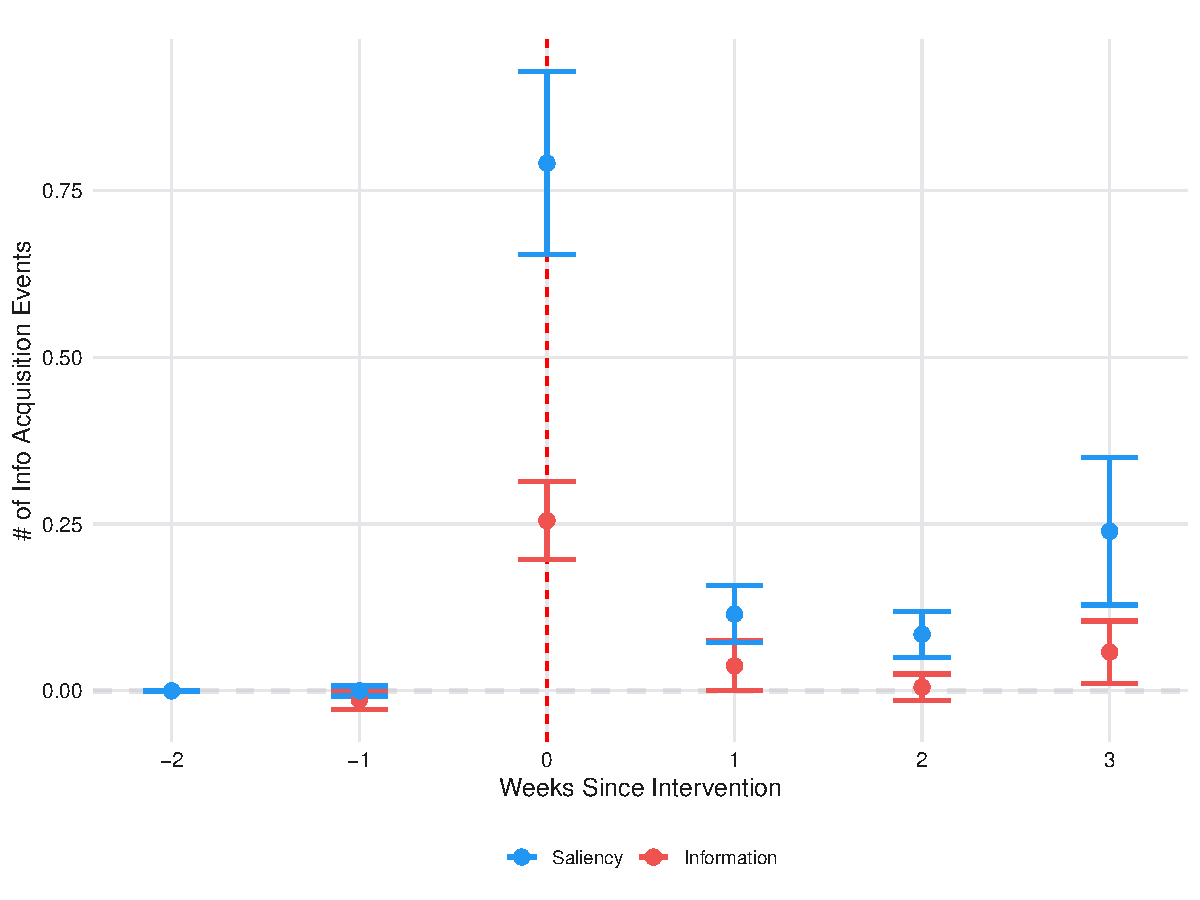
\includegraphics[width=0.6\textwidth]{./output/figures/info_acq_treatment_effects_total_sites.pdf}
\caption*{\scriptsize \textsc{Notes}: Weekly difference-in-differences estimates of the treatment effect on the number of distinct sites searched, from Equation (5), with $T_i \in \{\text{Info}, \text{Saliency}\}$, individual fixed effects, and randomization block fixed effects. Standard errors clustered at the participant level. Time window: weeks $-2$ to $+3$ relative to intervention.}
\end{figure}

\subsubsection*{Does Search Lead to Learning?}
 
The critical question is whether this additional search translates into learning. Figure~\ref{fig:beliefs_by_search} plots mean belief error conditional on whether the participant engaged in information acquisition on each site, separately by treatment group.

\begin{figure}
\centering
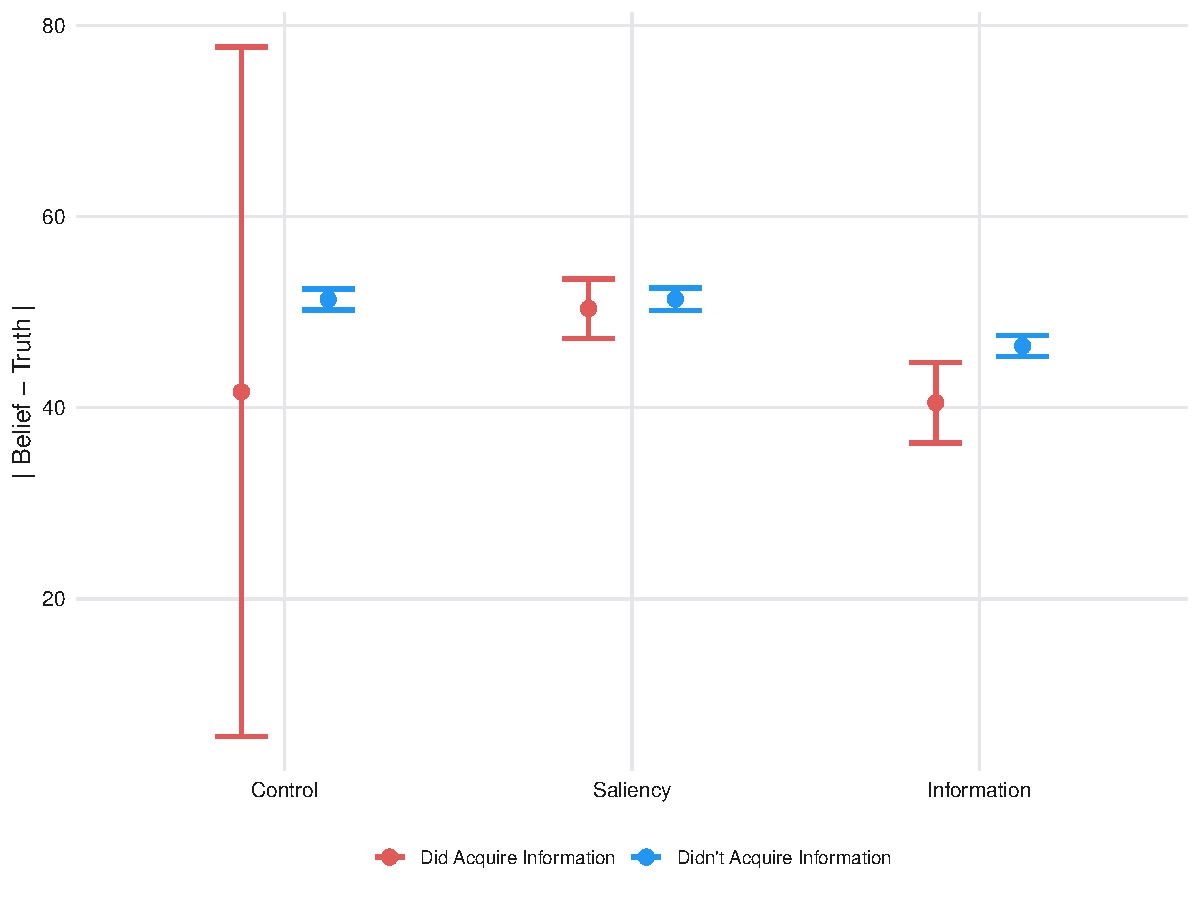
\includegraphics[scale=0.5]{./output/figures/beliefs_by_info_acq.pdf}
\caption{Beliefs by Search Behavior}\label{fig:beliefs_by_search}
  \centering
  \caption*{\scriptsize \textsc{Notes}: Weekly difference-in-differences estimates from Equation (5), with $T_i \in \{\text{Info}, \text{Saliency}\}$, individual fixed effects, and randomization block fixed effects. Standard errors clustered at the participant level. Time window: weeks $-2$ to $+3$ relative to intervention. Dependent variable is mean belief error $|\text{Belief} - \text{Truth}|$ conditional on engaging in privacy-related search (policy visit or dialog interaction).}
\end{figure}

Several patterns emerge. First, across all conditions, participants who engage in search have somewhat more accurate beliefs about the website's privacy practices than those who do not. Second, and most importantly, this difference is small and statistically insignificant for the saliency group: participants who searched for and read actual privacy policies are no more knowledgeable than those who did not. This result is consistent with privacy policy complexity being the binding constraint --- even motivated searchers cannot extract useful information from these documents.

Within the information group, participants who engaged in additional search beyond the popup have more accurate beliefs than those who relied on the popup alone. This holds even relative to the information group's higher baseline accuracy: non-searchers in the information group are more knowledgeable than searchers in the saliency group, consistent with the popup transmitting information even to participants who do not actively engage with it.

We note an important caveat: we are underpowered to precisely estimate the search--learning relationship in the control group, since very few control participants seek out privacy policies, which results in wide confidence intervals. This limits our ability to formally test Hypothesis 2(ii). However, the joint pattern across all three groups --- saliency participants search more but learn no more than control participants, while information participants learn substantially more whether or not they search --- provides strong evidence for Hypothesis 2(iii) and for complexity as the binding friction.

\medskip\medskip
 
\noindent The results of this section deliver a clean decomposition of the two information frictions in our model. Reducing search costs produces a dramatic increase in information-seeking behavior: the saliency treatment increases privacy policy visits by a factor of \policyVisitSaliencyFold{}. Yet this search is almost entirely unproductive --- saliency group participants are no better informed about the privacy practices of their most visited websites than control group participants. In contrast, reducing complexity through simplified, personalized disclosure produces meaningful improvements in belief accuracy, even among participants who do not actively engage with the information. The central lesson is that the binding constraint on privacy information acquisition is not access but comprehension: participants can find privacy policies but cannot learn from them.

\section{Effect on Website Choices}\label{sec:website_choice}

The results of Section~\ref{sec:hyp_info_beliefs} establish that the information treatment successfully transmits knowledge about privacy practices. The central question is whether this learning translates into changes in website choices. \gadelete{We examine two margins: data sharing (Section~\ref{sec:website_choice}) and website choice (Section~\ref{sec:website_choice}). We then corroborate these objective measures with self-reported behavioral changes from the endline survey (Appendix~\ref{sec:app-self-reported-changes}).}

Before presenting results, it is useful to set expectations about plausible magnitudes. Our conjoint estimates (Figure~\ref{fig:privacy_info_partworth}) imply that moving from a website that infringes on all three of a participant's most valued attributes to one that does not is worth approximately \$\wtpTopThreeMedian{} per month at the median. Meanwhile, the most popular websites in our data --- YouTube, Google, Amazon, Facebook --- have daily time-spent averages between \topWebFourActiveHours{} and \topWebOneActiveHours{} hours. Given the survey compensation rate of \$3 for 15 minutes of work, this implies a lower bound on the valuation of these sites of at least \$8.\footnote{It additionally dramatically dwarfs the overall valuation for these sites discussed in \cite{brynjolfsson2019using}.} % scalar 12 - not-reproducible
\mkcomment{old value was \$3, computed on a 1-unit change; my new value is \$\wtpTopThreeMedian{}, using the full $-1$ to $+1$ swing (2 units): each person's summed top-3 WTP, median across people. The \$8 quality lower bound I don't know how to compute, so left unchanged.} This crude approximation illustrates a significant gap: for the most frequently visited websites, quality-based valuations substantially exceed privacy costs. This means that large behavioral responses on the intensive margin --- participants abandoning their most-used sites --- are unlikely even if the information treatment is fully effective. The more plausible margin of adjustment is on the extensive margin, where participants shift among less-visited or marginal sites.
 
We now examine whether changes in beliefs lead to changes in the websites participants visit and how they allocate their time. Our model implies that the direction and magnitude of behavioral effects depend on beliefs ($\theta^b$), the intensity of privacy preferences ($\lambda^P$), quality differences across websites within a market, and the distribution of privacy practices. Consequently, aggregate effects are theoretically ambiguous and reduced-form magnitudes are difficult to interpret. We present results for both the intensive and extensive margins and interpret them in light of these considerations.

\subsection{Intensive Margin}
 
We first ask: holding the set of sites fixed, how does browsing behavior change? We construct a balanced panel for each participant across their full set of pre-treatment visited sites and estimate:
\begin{equation}
    y_{ijt} = \beta \cdot (\mathbf{1}\{\text{Post}\} \cdot T_i) + \eta_j + \eta_i + \epsilon_{ijt}
\end{equation}
where $\eta_j$ and $\eta_i$ are site and participant fixed effects.
 
Figure~\ref{fig:intensive_a} presents results for log time spent and the number of visits. Across both dependent variables, there is no evidence of changes in the intensive margin of browsing behavior. Importantly, our estimates are precise: the largest effects within our confidence intervals would imply changes of less than one minute in time spent or two additional visits over a two-week period --- less than 0.1\% of average time spent online.

\begin{figure}[H]
    \centering
    \caption{Browsing Behavior Treatment Effects: Intensive Margin}
    \label{fig:intensive}
    
    \begin{subfigure}[t]{0.4\textwidth}
        \centering
        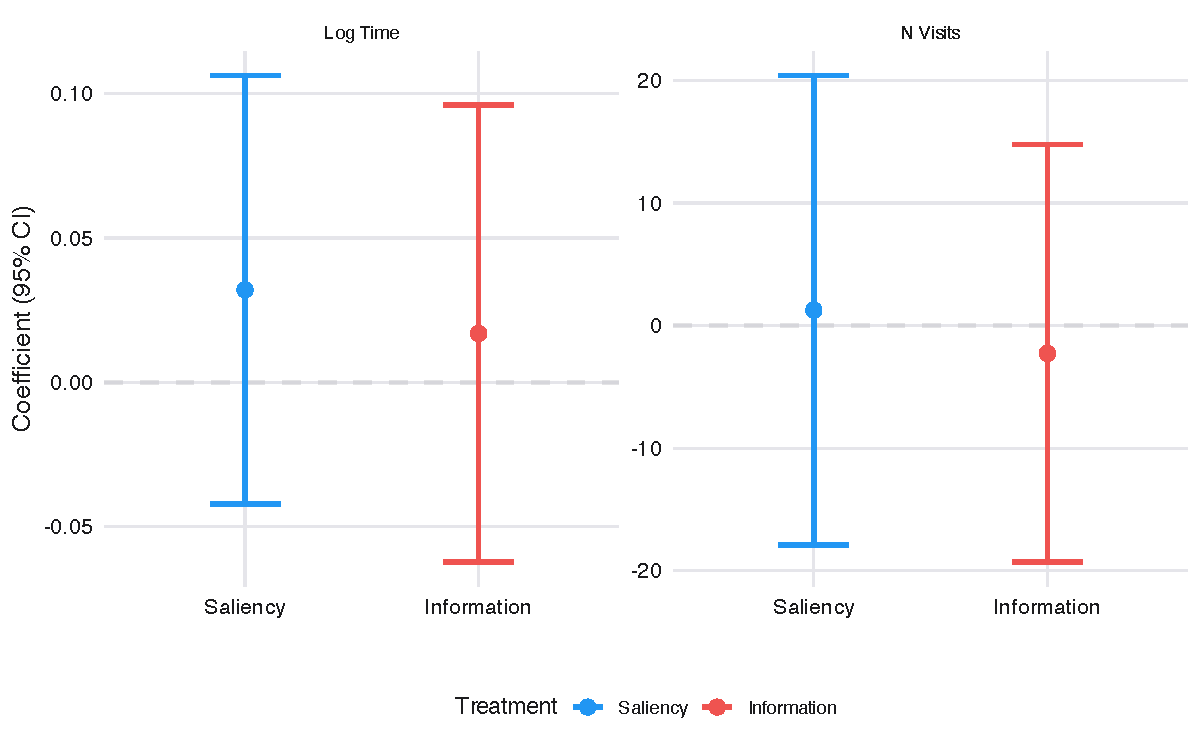
\includegraphics[width=\linewidth]{./output/figures/preregistered_spec_i_baseline.pdf}
        \caption{Difference-in-differences ATE}
        \label{fig:intensive_a}
    \end{subfigure}
    \hfill
    \begin{subfigure}[t]{0.4\textwidth}
        \centering
        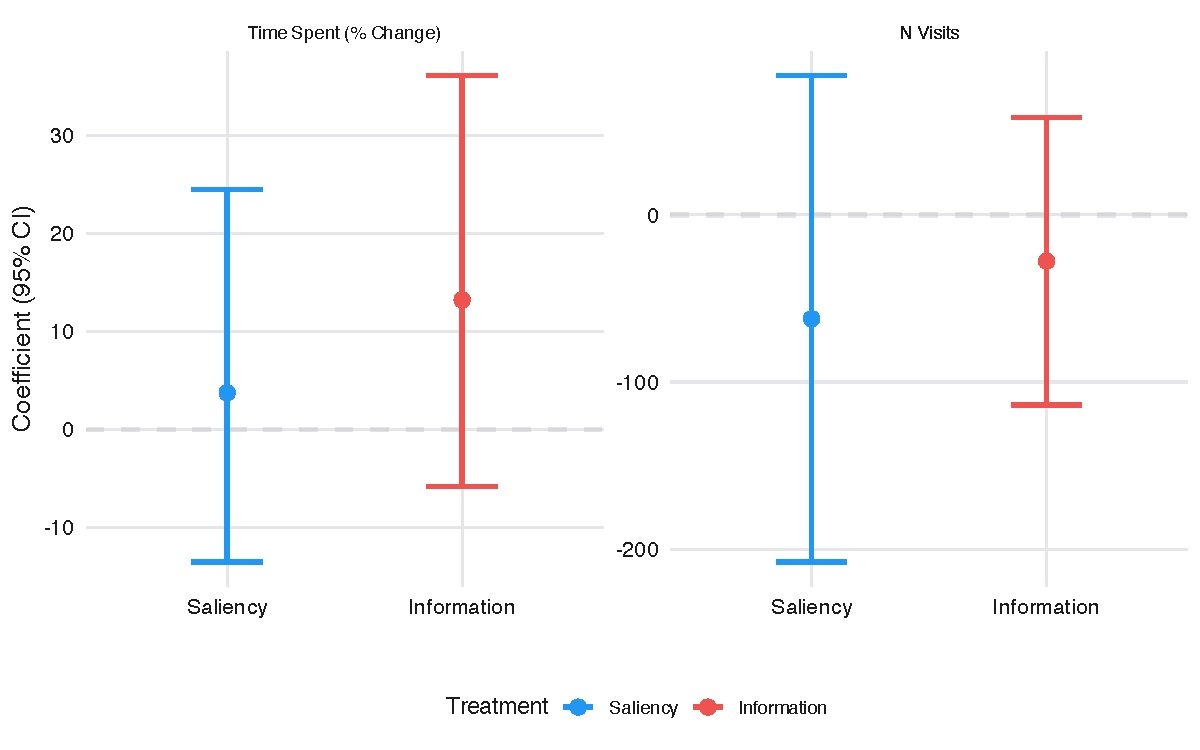
\includegraphics[width=\linewidth]{./output/figures/preregistered_triple_interaction_baseline.pdf}
        \caption{Triple Difference-in-differences: Heterogeneous ATE by Privacy Score}
        \label{fig:intensive_b}
    \end{subfigure}
    \caption*{\scriptsize \textsc{Notes}:  Panel (a): Difference-in-differences estimates from Equation (6). Outcomes: log time spent and visit count for individual $i$ on website $j$ in period $t$. Includes website and individual fixed effects. Sample restricted to balanced panel of websites visited in both baseline weeks ($t \in \{-2, -1\}$). Standard errors clustered at the participant level. Panel (b): Triple-difference estimates with privacy heterogeneity from Equations (7)–(8). Privacy score $P_{ij}$ computed per Equation (4), weighting site-level privacy attributes by individual $i$'s conjoint coefficients for personalized attributes $k \in \{1,2\}$. Outcomes winsorized at 5th and 95th percentiles. }
\end{figure}
 
This null is unsurprising given the valuation gap discussed above. The sample used here consists primarily of sites that participants spend significant time on and thus likely have strong preferences for. Observing large changes in these regressions would require participants to move away from their highest-value sites, which our WTP estimates suggest is unlikely.
 
Our model further implies that even if aggregate time on a site does not change, how participants allocate time \emph{across} sites may shift. To test this, we construct site-user-level privacy scores by weighting site-level privacy attributes by individual-level conjoint utility estimates. We then estimate a heterogeneous treatment effect specification:
\begin{equation}
    y_{ijt} = \beta(\mathbf{1}\{\text{Post}\} \cdot T_i \cdot P_{ij}) + \eta_j + \eta_t + \eta_i + \epsilon_{ijt}
\end{equation}
where $P_{ij}$ is our individual measure of privacy invasiveness. Figure~\ref{fig:intensive_b} presents the results and mirrors the aggregate findings: there is no evidence that participants differentially reallocate time toward or away from sites based on their privacy characteristics.

\subsection{Extensive Margin}
 
Given the valuation gap, the more plausible margin of adjustment is the extensive margin: how participants change the \emph{set} of sites they visit, particularly among less-visited or marginal sites. We assess this at the participant--category level using:
\begin{equation}
    Y^{\text{post}}_{ic} - Y^{\text{pre}}_{ic} = \beta \cdot T_i + \eta_c + \varepsilon_{ic}
\end{equation}
where the dependent variable is the within-user pre--post difference and $\eta_c$ is a category-level fixed effect.

\begin{figure}
    \centering
    \caption{Browsing Behavior Treatment Effects: Extensive Margin}
    \label{fig:extensive}
    
    \begin{subfigure}[t]{0.4\textwidth}
        \centering
        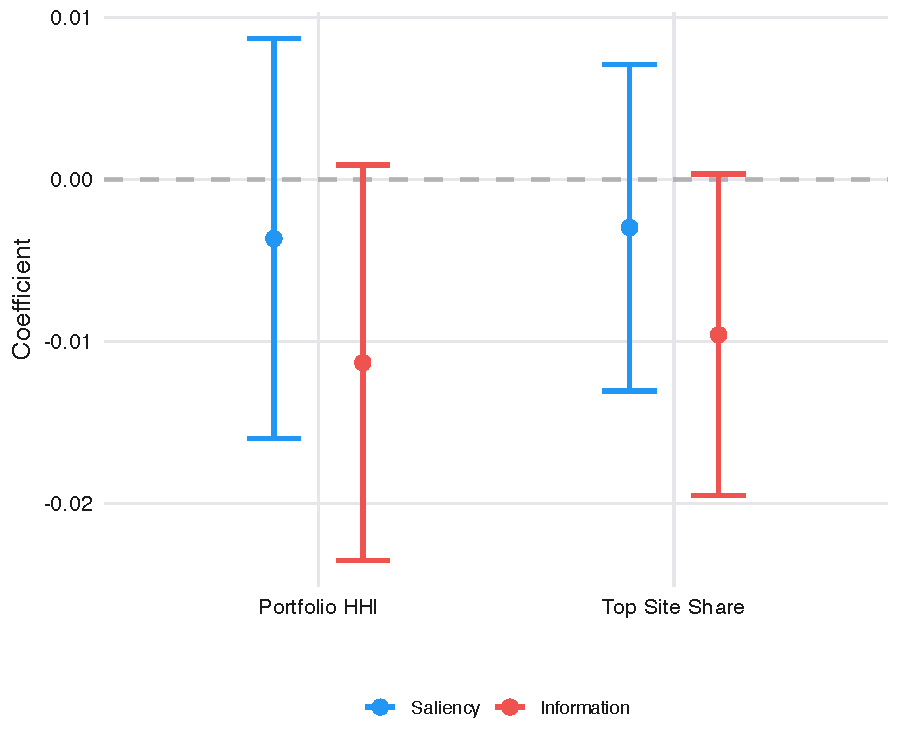
\includegraphics[width=\linewidth]{./output/figures/assortment_concentration.pdf}
        \caption{Assortment Changes within Category}
        \label{fig:extensive_a}
    \end{subfigure}
    \hfill
    \begin{subfigure}[t]{0.4\textwidth}
        \centering
        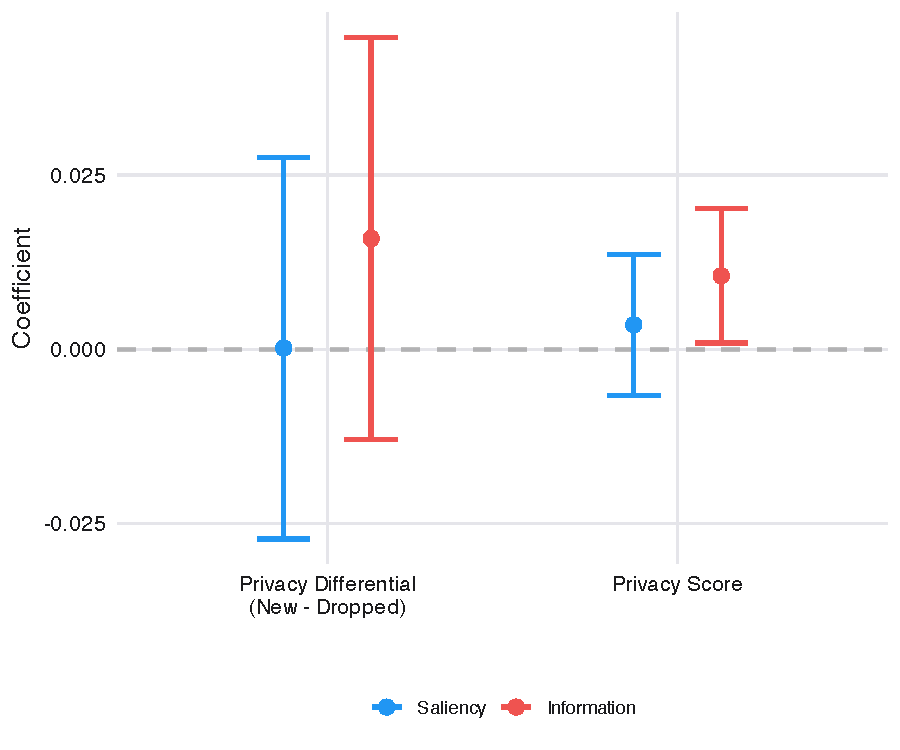
\includegraphics[width=\linewidth]{./output/figures/assortment_privacy.pdf}
        \caption{Experienced Privacy within Category}
        \label{fig:extensive_b}
    \end{subfigure}
    \caption*{\scriptsize \textsc{Notes}: First-difference estimates from Equation (9), where $\Delta Y_{ic} \equiv Y_{ic,\text{post}} - Y_{ic,\text{pre}}$ for individual $i$ in website category $c$. Includes category fixed effects. Standard errors clustered at the participant level. Panel (a): Concentration measures. HHI computed as $\sum_j s_{ijc}^2$, where $s_{ijc}$ denotes individual $i$'s time share on website $j$ within category $c$. Top-site share defined as $\max_j s_{ijc}$. Panel (b): Privacy measures. Sites classified as new if $s_{ijc,\text{pre}} = 0$ and $s_{ijc,\text{post}} > 0$; dropped if the reverse. Privacy differential computed as $\bar{P}_{i,\text{new}} - \bar{P}_{i,\text{dropped}}$, averaging site-level privacy scores within each group. Time-weighted privacy score computed as $\sum_j s_{ijc} \cdot P_{ij}$.}
\end{figure}
 
Figure~\ref{fig:extensive_a} presents results for two measures of browsing concentration: the Herfindahl--Hirschman Index (HHI) at the user--category level and the share of time spent on a participant's top 2 sites. Both regressions show small decreases in concentration for the information group, with p-values of \extensiveHHIPvalue{} (HHI) and \extensiveTopSharePvalue{} (top-2 share). While only marginally significant, the direction is consistent with participants diversifying their browsing in response to the information treatment.
 
Figure~\ref{fig:extensive_b} examines whether this diversification is privacy-motivated. We construct two measures. First, the \emph{privacy differential} between newly visited and dropped sites, capturing whether sites that participants begin visiting have better privacy practices than the sites they stop visiting. Second, the change in the average privacy score of each participant's portfolio of websites. The information group shows positive effects on both measures: the treatment accounts for approximately \privacyDifferentialPctSD{}\% of the standard deviation in the privacy differential and \portfolioPrivacyPctSD{}\% in the portfolio privacy score. These are modest magnitudes, but they indicate that the direction of extensive-margin reallocation is toward more privacy-conscious sites.

\noindent Cumulatively, the results of this section paint a consistent picture. Participants in the information group make small but detectable adjustments: they are somewhat more likely to opt out of data sharing and they modestly shift their browsing toward more privacy-conscious sites on the extensive margin. However, the intensive margin of browsing --- where participants spend the bulk of their time --- is essentially unchanged. This pattern is consistent with the valuation gap between website quality and privacy costs: for the sites that dominate participants' browsing, quality-based preferences are simply too strong for privacy information, even when personalized and simplified, to meaningfully alter behavior. We confirm that these are consistent with participants self-reported changes during the experiment using open-ended responses in the endline survey (see Appendix \ref{sec:app-self-reported-changes} for more details).
 
These reduced-form results, while informative about the direction and approximate magnitude of behavioral responses, face important limitations. The theoretical ambiguity noted at the outset of this section --- that aggregate effects depend on the joint distribution of beliefs, preferences, quality, and privacy practices --- means that reduced-form estimates are difficult to map into welfare-relevant quantities. Moreover, the reduced-form approach cannot separately identify how much of the limited behavioral response reflects low privacy valuations versus high search or comprehension costs that persist even under treatment. Disentangling these forces requires a structural model that jointly estimates preferences, information frictions, and the value of website quality. We develop such a model in the next section.

\section{Empirical Model}\label{sec:empirical_model}

We now specify an empirical analog of the model in Section~\ref{sec:model_hypotheses} that we take to the panel and experimental data. The reduced-form results of Sections~\ref{sec:hyp_info_beliefs}--\ref{sec:website_choice} show that the information treatment moves beliefs and produces detectable shifts in \emph{which} sites consumers browse, with a much weaker response in \emph{how} time is allocated across visited sites. To convert these behaviors into welfare we need structure that (i) lets privacy operate both on the decision of which sites to browse and on the allocation of time across them, (ii) ties revealed browsing to the stated conjoint preferences through a small number of interpretable parameters, and (iii) accommodates the information frictions that govern whether a treatment moves beliefs at all.

We model browsing as a consider-then-choose problem. In each period a consumer forms a consideration set over websites and then allocates time across considered sites by a nested logit. Privacy enters both stages through the consumer's revealed valuation of each site's data practices, and a single stated-to-revealed wedge links that revealed valuation to the conjoint. This structure relies on consideration-set demand \citep{goeree2008limited}. Conditional on arriving on a website consumers choose whether to acquire information about privacy practices, trading-off the value of that information for future decision making and the costs associated with searching.

\subsection{Setup and the Stated-to-Revealed Wedge}

A consumer $i$ of latent type $g(i) \in \{1, \dots, G\}$ browses websites $j = 1, \dots, J$ over a sequence of days. Three objects are measured \emph{outside} the browsing model and treated as data: stated preferences $\beta^{\text{conj}}_i \in \mathbb{R}^{K}$ ($K = 19$ per-attribute marginal utilities from the baseline conjoint, Section~\ref{subsec:stated_privacy_prefs}); prior beliefs $\theta^b_i \in [0,1]^{K}$ about each site's practices (baseline survey, Section~\ref{sec:knowledge_top_sites}); and the CARA risk-aversion coefficient $\gamma_i$. Each site $j$ carries true privacy attributes $\mu^*_j \in \{0,1\}^{K}$ (hand-coded from policies, Section~\ref{sec:policydata}), a type-specific quality index $Q_{gj}$, observable cookie features $x_j = (\text{Pers}_j, \text{SA}_j)$ (personalization, ad-sharing), and a content-category (nest) assignment.

We link stated preferences (from the conjoint) to revealed behavior through a per-type wedge $\xi_g$,
\begin{equation}\label{eq:em_wedge}
  \beta_{ik} = \beta^{\text{conj}}_{ik} \, / \, \xi_{g(i)},
\end{equation}
where $\beta_{ik}$ is the consumer's \emph{revealed} privacy valuation. A value $\xi_g > 1$ means revealed browsing expresses weaker privacy sensitivity than the conjoint states---a quantitative measure of the privacy paradox. Equation~\eqref{eq:em_wedge} is the empirical counterpart of the privacy term $\lambda^p_i \mathbb{E}[\mu^*]$ in the theoretical payoff~\eqref{eq:utility}: it replaces a single scalar privacy weight with a $K$-vector of attribute valuations disciplined by the conjoint. Concentrating preferences through the conjoint in this way reduces what an unrestricted specification would treat as $G \times K$ free privacy parameters to the $G$ scalars $\xi_g$---themselves the first-order objects of interest---without severing the link to the elicited stated preferences.

Because the conjoint is framed monthly while the panel allocates time daily, the divisor in~\eqref{eq:em_wedge} is an \emph{effective} wedge that factors a units constant from a behavioral one, $\xi_g \equiv \xi^{\text{eff}}_g = D\,\xi^{\text{pure}}_g$, with $D = 30$ calendar days per month; we estimate the dimensionless paradox factor $\xi^{\text{pure}}_g$.\footnote{$D$ is a units constant, not a preference: it restates the monthly conjoint coefficient on the panel's daily frame. Embedding it is a one-to-one change of variables that leaves every moment unchanged at a given fit while centering the estimated $\xi^{\text{pure}}_g$ at $O(1)$. The timescale enters the model once---in welfare it is applied through each consumer's number of active browsing days (Section~\ref{sec:em_welfare}), not a second time through the price coefficient.}

\subsection{The Consideration Margin}

A site enters consumer $i$'s consideration set with probability $p^{\text{vis}}_{ij} = \Lambda(z_{ij})$, where $\Lambda(\cdot)$ is the logistic CDF and
\begin{equation}\label{eq:em_z}
  z_{ij} = \alpha^{\text{ext}}_g + \gamma^{\text{ext}} Q_{gj} + \phi_{\text{ext}}\, \CE_{ij} + \theta_{\text{persist}}\, v^{\text{pre}}_{ij}.
\end{equation}
Here $\alpha^{\text{ext}}_g$ is a type-specific consideration intercept, $\gamma^{\text{ext}}$ weights observable quality, $v^{\text{pre}}_{ij}$ is a habit stock (the consumer's pre-period visit history to $j$), and $\CE_{ij}$ is the CARA certainty equivalent of the site's privacy practices,
\begin{equation}\label{eq:em_ce}
  \CE_{ij} = \sum_{k} \beta_{ik}\,\theta_{ijk} \;-\; \frac{\gamma_i}{2} \sum_{k} \beta_{ik}^2\, \theta_{ijk}(1 - \theta_{ijk}).
\end{equation}
The first term is the expected privacy (dis)utility under current beliefs; the second is an uncertainty penalty---risk-averse consumers are less willing to consider sites about which their beliefs are diffuse ($\theta_{ijk}$ near $\tfrac12$). Privacy enters consideration \emph{only} through $\phi_{\text{ext}}\,\CE_{ij}$, where $\phi_{\text{ext}} \ge 0$ is the weight on privacy in the consideration index. Resolving uncertainty (shrinking the penalty) or correcting the mean both shift $p^{\text{vis}}_{ij}$, which is the channel through which the information treatment acts on browsing.

\subsection{Time Allocation}

Conditional on the consideration set, the flow utility from site $j$ is
\begin{equation}\label{eq:em_uint}
  u_{ij} = \lambda_g \bigl(Q_{gj} + \delta' x_j\bigr) + \CE_{ij},
\end{equation}
where $\lambda_g$ is the type-specific quality weight (the empirical analog of $\lambda^q_i$ in~\eqref{eq:utility}), $\delta = (\delta_{\text{Pers}}, \delta_{\text{SA}})$ is the cookie-feature contribution to site value,\footnote{Concretely $\delta' x_j = \delta_{\text{Pers}}\,\text{Pers}_j + \delta_{\text{SA}}\,\text{SA}_j$: cookies are valued for the personalization they enable, net of the disutility of downstream ad-sharing. The end-of-experiment cookie-deletion period supplies the exogenous within-consumer variation that identifies $\delta_{\text{Pers}}, \delta_{\text{SA}}$ and a deletion-period logging adjustment $\bar\pi$.} and the privacy coefficient on the intensive margin is normalized to one. Time shares across considered sites follow a nested logit, with nests equal to content categories and nest correlation $\sigma_{\text{nest}}$; the within-nest log share satisfies the standard inversion
\begin{equation}\label{eq:em_nl}
  \ln s_{ij} = \frac{u_{ij}}{1 - \sigma_{\text{nest}}} + \sigma_{\text{nest}} \ln \bar{s}_{i, n(j)} + \text{const},
\end{equation}
where $\bar{s}_{i,n(j)}$ is the within-nest share. The model thus produces, for each consumer--site--period, a consideration probability $p^{\text{vis}}_{ij}$ and a conditional time share $s_{ij}$; their product is the unconditional share used for welfare. Privacy enters time allocation through the same certainty equivalent $\CE_{ij}$~\eqref{eq:em_ce} as the consideration index, with its coefficient normalized to one, so the relative strength of privacy on the two margins is governed by $\phi_{\text{ext}}$ rather than by separate preferences. Both margins thus treat the consumer as risk-averse over the uncertain practices in the same way. Quality $Q_{gj}$, by contrast, is known and enters both margins \emph{linearly}, never inside the certainty equivalent: under CARA the risk premium is independent of the level of deterministic utility, so a site's quality does not scale its privacy risk, and the variance penalty in~\eqref{eq:em_ce} falls on the uncertain privacy component alone.\footnote{Equivalently, the certainty equivalent of a known quality plus a risky privacy bundle separates as $\CE[\lambda_g(Q_{gj}+\delta'x_j) + \text{privacy}] = \lambda_g(Q_{gj}+\delta'x_j) + \CE_{ij}$, a property of CARA (no wealth effects). Folding $Q_{gj}$ into the risk transform would instead impose increasing absolute risk aversion and is avoided.}

\subsection{Information Acquisition}

This stage operationalizes the two-step acquisition process of Section~\ref{sec:participant_model}. On visiting a site the consumer chooses whether to read its privacy policy, trading the value of resolving uncertainty against an acquisition cost
\begin{equation*}
  c_{ij} = c^s_{\text{base}} - \delta_{c_s}\,\mathbf{1}\{\text{saliency}\} + \varepsilon^s_{ij},
\end{equation*}
where $\varepsilon^s_{ij}$ is a normal taste shock; she searches when the value of information exceeds $c_{ij}$. The CARA--Bernoulli structure yields a closed-form value of information
\begin{equation}\label{eq:em_voi}
  \VOI_{ij} = \frac{\gamma_i}{2}\, \alpha_{\text{search}} \Bigl(\textstyle\sum_k \beta_{ik}^2\, \theta_{ijk}(1 - \theta_{ijk})\Bigr) M_g,
\end{equation}
with $M_g$ a type-specific count of browsing occasions over which resolved information is reused. Information is most valuable precisely where beliefs are uncertain and the revealed privacy stakes $\beta_{ik}$ are large---the same $\beta_{ik}$ that govern choice---which is what makes the saliency arm's search behavior informative about the privacy scale (Section~\ref{sec:identification}). Because these stakes are the \emph{revealed} $\beta_{ik} = \beta^{\text{conj}}_{ik}/\xi_g$, the wedge $\xi_g$ scales the value of information exactly as it scales browsing: we treat $\xi_g$ as a preference--behavior wedge that governs \emph{all} of the consumer's choices, information acquisition included, rather than a friction the consumer would privately wish to overcome. Conditional on searching, beliefs update imperfectly: after $n^{\text{pop}}_{ij}$ exposures,
\begin{equation}\label{eq:em_update}
  \Delta\theta_{ijk} = \Bigl[1 - (1 - \alpha_{\text{info}})^{\log(1 + n^{\text{pop}}_{ij})}\Bigr]\bigl(\mu_{jk} - \theta_{ijk}\bigr),
\end{equation}
and voluntary policy reading adds an analogous term in $\alpha_{\text{search}}$ and the voluntary-search count, the two channels composed additively and clipped to $[0,1]$. The weight on the truth, $w \equiv 1 - (1-\alpha_{\text{info}})^{\log(1 + n^{\text{pop}}_{ij})} \in [0,1]$, makes each posterior a convex combination $(1-w)\theta_{ijk} + w\mu_{jk}$ of prior and truth---a saturating partial-adjustment rule in which $\alpha_{\text{info}}$ is the per-exposure comprehension probability (the consumer absorbs the truth if at least one effective exposure succeeds), the $\log(1+n^{\text{pop}})$ dosage imposes diminishing returns to repeated popups, and beliefs reach the truth only in the limit $n^{\text{pop}} \to \infty$. The experimental arms map cleanly onto these primitives (Section~\ref{sec:experiment}): the saliency arm lowers the search cost ($\delta_{c_s} > 0$); the information arm additionally lowers complexity (raises $\alpha_{\text{info}}$); the control arm induces no structural belief update.

\subsection{Welfare}\label{sec:em_welfare}

We measure welfare by the inclusive value:
\begin{equation}\label{eq:em_iv}
  CS_i = \log\!\Bigl(1 + \sum_{n} \Bigl[\textstyle\sum_{j \in n} p^{\text{vis}}_{ij} \exp\!\bigl(u_{ij}/(1 - \sigma_{\text{nest}})\bigr)\Bigr]^{1 - \sigma_{\text{nest}}}\Bigr),
\end{equation}
Following \citet{train2015} we evaluate \emph{experienced} rather than perceived welfare: the intensive utilities $u_{ij}$ are computed at the true practices $\mu^*_j$, while consideration $p^{\text{vis}}_{ij}$ is driven by the consumer's (possibly mistaken) beliefs---consumers act on beliefs but enjoy realized utility. The cost of privacy is the surplus difference between the estimated model and a counterfactual that switches off privacy invasive practices (or turns on privacy protective ones), decomposed across the two margins,
\begin{equation*}
  \underbrace{CS^{\text{np}}_i - CS_i}_{\text{total}} = \underbrace{\bigl(CS^{\text{np}}_i - CS^{\text{ext}}_i\bigr)}_{\text{extensive (which sites)}} + \underbrace{\bigl(CS^{\text{ext}}_i - CS_i\bigr)}_{\text{intensive (time} \mid \text{visit)}},
\end{equation*}
where $CS^{\text{ext}}_i$ retains privacy in consideration but removes it from the intensive utility. Counterfactuals (full information, attribute bans) replace the relevant beliefs or practices and recompute~\eqref{eq:em_iv}. Per-day utilities are converted to dollars with each consumer's own conjoint price coefficient $1/|\beta_{\text{price},i}|$ and summed over the days the consumer actually browses. The privacy \emph{share} of surplus is invariant to the price coefficient, and to the day aggregation, whereas the dollar \emph{level} scales as $1/\xi^{\text{eff}}$.

\section{Estimation}\label{sec:estimation}

We estimate $\theta$ by two-step GMM \citep{hansen1982large}. The parameter vector is
\begin{equation*}
  \theta = \bigl(\xi_g,\, \phi_{\text{ext}},\, \alpha^{\text{ext}}_g,\, \gamma^{\text{ext}},\, \sigma_{\text{nest}},\, \lambda_g,\, \delta_{\text{Pers}}, \delta_{\text{SA}},\, c^s_{\text{base}}, \delta_{c_s},\, \alpha_{\text{info}}, \alpha_{\text{search}},\, \bar\pi,\, \theta_{\text{persist}}\bigr),
\end{equation*}
$11 + 3G$ parameters, where the type-subscripted $\xi_g, \alpha^{\text{ext}}_g, \lambda_g$ each collect $G$ values and the intensive-margin privacy coefficient is normalized to one. Site quality is not a free parameter: at each evaluation the type-specific $Q_{gj}$ is concentrated out by a Berry-style contraction \citep{berry1994estimating} that equates model and observed per-type shares, absorbing each type's baseline per-site appeal so the structural parameters are identified from the experiment and privacy-driven reallocation rather than from cross-sectional taste.

\subsection{Type Classification}

The latent types are formed in a preliminary step, prior to estimating $\theta$. Following \citet{bonhomme2022}, we discretize unobserved heterogeneity into $G$ types by model-based clustering on pre-treatment data. Each consumer is summarized by a feature vector that stacks three sources measured before the information intervention: baseline beliefs $\theta^b_i$ (the $K$ survey priors), risk aversion $\gamma_i$, and the consumer's baseline browsing vector (per-site $\log(1+\text{time share})$ over the pre-treatment window). Including the browsing outcomes follows the \citet{bonhomme2022} prescription of grouping on the high-dimensional moment vector that the structural model must reproduce. We reduce the stacked features by principal components (retaining 90\% of the variance) and fit a Gaussian mixture model, selecting its covariance structure by BIC. The types are then held fixed in the GMM, governing the quality weight $\lambda_g$, the consideration intercept $\alpha^{\text{ext}}_g$, and the wedge $\xi_g$.

\section{Moment Conditions and Identification}\label{sec:identification}\label{sec:em_moments}

We estimate $\theta$ against nine moment blocks of the common form
\begin{equation}\label{eq:em_moment}
  m_b = \E\bigl[\bigl(y^{\text{obs}}_{i} - \hat y_{i}(\theta)\bigr)\, z_{i}\bigr] = 0,
\end{equation}
the average over consumers---within type $g$, and arm where relevant---of a residual between an empirical target $y^{\text{obs}}$ and its model prediction $\hat y(\theta)$, weighted by an instrument or treatment contrast $z$ (with $z \equiv 1$ where the block matches a level). Each block below specifies its own $y^{\text{obs}}$, $\hat y$, and $z$. Identification rests on the experiment's three-way variation---the baseline period (control, days 1--14) anchors structural levels free of treatment, the saliency arm exogenously lowers search cost, and the information arm exogenously corrects beliefs---so that, with $a \in \{\text{control}, \text{saliency}, \text{info}\}$ indexing arms and $Z_{ijk} = \mu_{jk} - \theta_{ijk}$ the belief gap, info$-$control contrasts isolate the privacy channel from quality, habit, and search cost. Two recursive notes organize what follows. First, the latent types are separated by their baseline visit volumes and quality gradients (Block $V$) and their cookie-deletion responses (Block $E$), so the type-specific objects $\lambda_g, \alpha^{\text{ext}}_g, \xi_g$ are anchored to observable type differences. Second, the belief-update magnitude is pinned down separately from the privacy response. The information treatment moves behavior through the product of how far beliefs shift ($\alpha_{\text{info}}$) and how strongly browsing responds to that shift (the privacy scale); without separately measuring how far beliefs move, a muted response could mean either that consumers barely learned or that they learned but do not act on privacy. Block $B$ resolves this by identifying $\alpha_{\text{info}}$ from endline belief accuracy rather than from behavior, so the privacy blocks $C_{\text{int}}, T, P$ can attribute the residual response to privacy sensitivity rather than to a smaller belief shift. We group the blocks below by the object they discipline; Table~\ref{tab:em_identification} lists each block's size and the parameters it pins down. 

\begin{table}[ht]
\centering
\caption{Parameters, Moments, and Identifying Variation}\label{tab:em_identification}
\begin{tabular}{@{}llcl@{}}
\toprule
Parameter & Moment(s) & Size & Identifying variation \\
\midrule
$Q_{gj}$ & BLP inner loop & --- & model $=$ observed aggregate time shares, by type \\
$\lambda_g$ & $E$, intensive levels & --- & cookie-deletion response; quality scaling of shares \\
$\delta_{\text{Pers}}, \delta_{\text{SA}}$ & $E$ & \multirow{2}{*}{$3$} & change in browsing by cookie feature at deletion \\
$\bar\pi$ & $E$ & & post-deletion level shift \\
$\sigma_{\text{nest}}$ & $F$ & $6$ & within- vs.\ across-nest substitution (diff.\ IVs) \\
$\alpha^{\text{ext}}_g$ & $V$ & \multirow{2}{*}{$6$} & baseline number of sites visited, by type \\
$\gamma^{\text{ext}}$ & $V$ & & baseline mean quality $\mid$ visited \\
$\theta_{\text{persist}}$ & $R$ & $9$ & return rate to previously visited sites \\
$c^s_{\text{base}}$ & $A$ & \multirow{2}{*}{$7$} & control-arm search (policy-read) level \\
$\delta_{c_s}$ & $A$ & & saliency $-$ control search differential \\
$\alpha_{\text{info}}$ & $B$ & \multirow{2}{*}{$6$} & info $-$ control belief-accuracy gain \\
$\alpha_{\text{search}}$ & $B$ & & belief gain from voluntary search (saliency) \\
$\xi_g$ & $C_{\text{int}}, P, A$ & $3{,}\,9$ & disclosure dose-response; visited-set privacy shift; VOI slope \\
$\phi_{\text{ext}}$ & $T, P$ & $18{,}\,9$ & magnitude of treatment visit / privacy-exposure response \\
\bottomrule
\end{tabular}
\end{table}

\paragraph{Privacy scale.} The revealed privacy strength is identified from how sharply browsing responds when the information treatment corrects beliefs about specific sites. Learning that a site is more invasive than she thought pushes a privacy-sensitive consumer away from it---fewer visits, less time---while better-than-expected news pulls her toward it; the size of this reallocation per unit of belief correction is the scale we want to recover. Two features of the design rule out the obvious confounds: the treatment randomizes \emph{which} practices are disclosed, so the response attaches to specific attributes rather than to unobserved site appeal, and the magnitude of the correction is pinned down separately, so the response reflects how much consumers act on privacy rather than how surprising the news was.

We operationalize this with three moments. (1) \emph{Block $C_{\text{int}}$} (intensive margin) matches the info$-$control change in log time-share-conditional-on-visit to its nested-logit prediction from the belief-update-induced change in the certainty equivalent~\eqref{eq:em_ce}, weighting by the belief gap aggregated over the attributes actually disclosed at $(i,j)$---the persistent attributes shown to $i$ plus the randomly assigned attribute at site $j$, whose exogeneity makes the disclosure response informative about the scale. (2) \emph{Block $P$} (extensive margin) matches, by type and arm, the privacy exposure $\sum_k \mu^*_{jk}\beta_{ik}$ of the sites a consumer visits. Its info$-$control shift---consumers moving toward less invasive sites under the treatment---is the structural counterpart of the assortment response in Section~\ref{sec:website_choice}. (3) The saliency arm supplies a third source of identification: search responds more steeply to the value of resolving a site's uncertainty when the consumer cares more about privacy (\emph{Block $A$}, below). Because the same $\beta_i$ enters both margins, the extensive response alone identifies only the ratio $\phi_{\text{ext}}/\xi$; the intensive and search responses, which move with $\xi$ alone, separate it from $\phi_{\text{ext}}$.

\paragraph{Information frictions.} Whether the information treatment changes behavior at all turns on two frictions: how costly it is to find and attend to a site's privacy information, and how much of it consumers absorb once they do. The experiment is designed to separate them---the saliency arm lowers the cost of looking, the information arm additionally simplifies what is found---and two blocks recover them directly from the data. (1) \emph{Block $A$} (search) matches how often consumers read privacy policies: the baseline rate identifies the search cost, the jump under the saliency treatment identifies how much it falls, and searching more at sites where information is more valuable also identifies the privacy scale (the channel previewed above).  (2) \emph{Block $B$} (comprehension) matches endline belief accuracy: how far beliefs move toward the truth identifies the information arm's learning rate, against the near-zero gain from policy-reading alone in the saliency arm.

\paragraph{Demand and dynamics.} The remaining five blocks pin down the non-privacy structure of browsing---how appealing sites are at baseline, how consumers substitute across them, and how persistent their habits are---so that it is not confounded with the privacy responses; each matches an observed statistic to its model prediction. (1) \emph{Block $V$} (baseline consideration) matches, for each type, the mean number of distinct sites a consumer visits before treatment and the mean quality of those sites, which together fix the level and quality-gradient of consideration. (2) \emph{Block $T$} (treatment extensive) matches those same two statistics during the treatment period, by type and arm, so that the model reproduces the experiment's effect on how many and which sites consumers visit. (3) \emph{Block $E$} (cookie deletion) uses the staggered cookie-deletion rollout, matching the difference-in-differences in log time-share projected onto the personalization and ad-sharing features and an early-cohort indicator. (4) \emph{Block $F$} (nesting) identifies the substitution structure by projecting the demand residual onto differentiation instruments in the spirit of \citet{berry1995automobile}---within-nest counts and squared distances, consumer-demeaned. (5) \emph{Block $R$} (state dependence) matches the rate at which consumers return to sites they have visited before, by type and arm.

\section{Conclusion}

This paper demonstrates that while participants value privacy and hold systematically biased beliefs about website data practices, the effectiveness of privacy information provision depends on reducing information complexity as well as reducing search costs. In a large-scale field experiment with nearly 1,600 participants, we find that making privacy policies salient increases search behavior by a factor of \policyVisitSaliencyFold{} but produces no improvement in knowledge about privacy practices, whereas providing simplified, personalized privacy information improves belief accuracy by \beliefCorrectStrictInfoPP{} percentage points. Despite this learning, behavioral responses were modest: participants show limited changes on the intensive margin of website usage, with small but detectable shifts toward privacy-conscious sites on the extensive margin.

Using the resulting data and experimental variation, we estimate a structural consideration-set model of browsing choices and privacy information acquisition (Section~\ref{sec:empirical_model}) in which privacy preferences operate on both the extensive margin (which sites consumers consider) and the intensive margin (how they allocate time across considered sites), linked to stated conjoint preferences through a single stated-to-revealed wedge $\xi_g$. Privacy enters the consideration stage through a certainty-equivalent of each site's data practices and the time-allocation stage through the same revealed valuation, so the relative strength of the two margins is an output of estimation rather than an imposed restriction. The wedge $\xi_g$ quantifies the privacy paradox on the revealed-behavior scale, and the model recovers the value of privacy together with the welfare effects of information provision and attribute regulation.

We evaluate two key provisions of privacy regulation: information provision and restriction of specific privacy attributes. We show that there are meaningful welfare gains from both---eliminating search and information frictions leads to a welfare gain of \$16 per consumer per month and GDPR-style attribute restrictions yield a welfare gain of \$32 per consumer per month. Privacy costs and counterfactual welfare gains operate entirely through the extensive margin, and GDPR-style regulation generates welfare gains only through consumer reallocation---regulations that consumers do not observe or respond to produce no welfare improvement. This suggests that disclosure policies should target the visit decision (e.g., warnings before first visit, browser-level privacy ratings) and that regulation is only effective to the extent that it is communicated to consumers.

\bibliographystyle{chicago}
\bibliography{refs}
\newpage
 \counterwithin{figure}{section} % needed for numbering figures in the appendices
\counterwithin{table}{section}
\begin{appendix}

\section{Data Collection Appendix}\label{sec:data_collection_appendix}


\begin{table}[H]
  \centering
  \caption{Privacy Policy Feature Descriptions}\label{tab:characteristics}
  \scalebox{.8}{
  \begin{tabular}{|p{0.15\textwidth}|p{0.15\textwidth}|p{0.25\textwidth}|p{0.55\textwidth}|}
    \hline
    \textbf{Feature} & \textbf{Field} & \textbf{Short Description} & \textbf{Long Description} \\
    \hline
    use & law & Law Enforcement & Your user data may be shared with law enforcement. \\
    \hline
    use & ads & Advertising Partners & Your user data may be shared with advertising partners. \\
    \hline
    use & finance & Financial Transactions & Your user financial transaction information may be shared with other parties. \\
    \hline
    use & social-media & Social Media & Your user data may be shared with social media platforms. \\
    \hline
    use & partners & 3rd Party Partners & Your user data may be shared with 3rd party partners (non-advertising business partners). \\
    \hline
    use & service & 3rd Party Services & Your user data may be shared with 3rd party services (service providers or other businesses). \\
    \hline
    use & personalization & Website Personalization & You can choose to let the website personalize content for you, without sharing your data with partners. \\
    \hline
    collect & log & Browsing On-site & Your browsing behavior on and across the current website may be collected. \\
    \hline
    collect & offsite & Browsing Off-Site & Your browsing behavior off the current website may be collected. \\
    \hline
    collect & sensitive & Sensitive Personal Info & Your sensitive personal user information (religious affiliation, sexual orientation, political beliefs, etc.) may be collected. \\
    \hline
    collect & financial & Financial Data & Your financial information (purchase history, credit card information, etc.) may be collected if available. \\
    \hline
    collect & bio & Demographic Data & Your demographic data (gender, race, etc.) may be collected if available. \\
    \hline
    collect & location & Location & Your location data may be collected if available. \\
    \hline
    collect & social-media & Social Media Info & Your social media account information (and possibly associated behavior) may be collected, if available. \\
    \hline
    control & storage & Data is secured & The privacy policy specifies whether the collected data is properly secured. \\
    \hline
    control & anonymized & Data is anonymized & The privacy policy specifies whether the collected data is properly anonymized. \\
    \hline
    control & automated & Automated Deletion & Your data will be automatically deleted after a specified time period. \\
    \hline
    control & change & Notification of Change & You will be notified if there is a material change to the privacy policy. \\
    \hline
    control & deletion & Data Deletion & You have the ability to request the deletion of your data, but your data is not automatically deleted. \\
    \hline
  \end{tabular}
  }
\end{table}

\noindent \textbf{Chrome Extension}: We discuss additional technical details regarding the Chrome Extension that we use in the study. This extension is developed to automatically collect information on data collection and provide information to users overlaid on their normal web experience.

The automatic data collection done by the Chrome Extension uses the same underlying detection mechanisms that power the popular open-source AdBlockPlus extension. Both AdBlockPlus and our extension use the continually updated rules from \url{easylist.to} that allow for detection of network requests to third party advertising and analytics firms as well as which HTML elements are advertisements. Our software extends the implementation from AdBlockPlus to enable directly reading metadata sent (e.g., cookies) via network requests. This provides us with data on the identity of 3rd party cookies and network requests. Beyond this, our extension also provides an implementation of robust time tracking across pages and websites that accounts for possible user idleness.

There are several important technical details that are relevant for compliance and data collection. First, our extension can uniquely identify each participant, as they are required to input their randomly assigned experiment ID when they enter into the study. Second, the extension logs an internal identifier that is maintained so long as the extension is installed. If the participant uninstalls the extension, then the timestamp, along with both identifiers, is recorded in our servers. Participants receive an automated email indicating that they have opted out of the study upon uninstalling. Thus, we can observe compliance with the experiment via the extension. Finally, all of our collected data (via the extension) is persisted and stored on our servers at an interval of one minute -- ensuring we can continuously collect data as long as the extension is installed.

\vspace{0.5cm}

\noindent \textbf{Privacy Policy Classification \& Construction of Privacy Characteristics}: To gauge the space of relevant privacy characteristics, we first ran an open response survey asking ``What website characteristics do you consider privacy invasive? What website behaviors do you consider privacy enhancing?" Then, using sources such as \url{https://pirg.org/resources/how-to-read-a-privacy-policy/},  \url{ https://usableprivacy.org/data} and consultation with legal experts we have constructed an exhaustive set of privacy relevant, internet service attributes. The attributes cover a variety of topics such as security, storage, sharing and selling of data, and rights. These sets of attributes are presented below in Table \ref{tab:characteristics}.

We use the tracker data collected by the Chrome Extension to provide validation for our labeled privacy characteristics. Across our entire dataset, we observe nearly 30,000 unique third party domains that are shared data and nearly 1.5 million unique trackers. % scalar 15 - not-reproducible
In order to ensure that we are able to accurately match these domains to their purpose, we rely on four external sources to classify them. The primary external source that we rely on comes from Third Party Web which pulls data from the HTTP Archive and provides classifications of the purpose for each request \footnote{\url{https://www.thirdpartyweb.today/about}}. In addition, we supplement our classifications with data from Ghostery\footnote{\url{ https://github.com/ghostery/trackerdb}}, WhoTracksMe\footnote{\url{https://github.com/whotracksme/whotracks.me}}, and Cloudflare Radar\footnote{\url{https://radar.cloudflare.com}} to improve the coverage. The final classification is therefore assigned in a two-stage process. First, we query the sources in a descending priority of Third Party Web, Ghostery, WhoTracksMe, and finally Cloudflare Radar. Second, we align all final categories to the Third Party Web taxonomy for consistency, as this source empirically classifies the most trackers.

Since our tracker data captures analytics data collection, we focus on the `Browsing on-site data' measure from Table \ref{tab:characteristics}. If we observe the presence of any of the analytics trackers then this reliably indicates that the website is engaged in this practice. Table \ref{tab:conf_matrices} provides the confusion matrix between the tracker and policy data for the 500 websites for which we have policy data and shows that there is general alignment between the two measures.


\begin{table}[ht]
\centering
\caption{Confusion Matrix for Analytics Data}
\label{tab:conf_matrices}
\begin{tabular}{ccccc}
& & \multicolumn{2}{c}{Detect} & \\
 & & Tracker: No & Tracker: Yes & \\
\hline
\multirow{2}{*}{Claim} & Policy: No & 1 & 11 \\
 & Policy: Yes & 26 & 458 \\
\hline
\\[-1.5ex]
\end{tabular}
\end{table}
% scalar 16 - not-reproducible



\section{Conjoint Details}\label{sec:conjoint_details}

In this section, we detail the conjoint method used to measure participant's stated preferences for privacy attributes. Conjoint experiments consist of a number of tasks. Each task presents a participant with a set of theoretical products which may vary across some set of characteristics, for example price, and asks the participant which product they would most like to purchase. Participants repeat this task multiple times, with product sets and characteristics varying across tasks. Thus, a conjoint experiment generates exogenous variation in product characteristics and choice sets, allowing for the estimation of preferences. As these choices tasks are entirely hypothetical, estimated preferences are reflective of stated-preferences. Yet, conjoint presents a systemized way of eliciting preferences that has been shown to contribute to more reliable as well as internally and externally valid estimates \citep{ALLENBY2019151, doi:10.1287/inte.31.3s.56.9676}. 

Our goal is to elicit preferences for the 19 privacy practices we measure. Our conjoint proceeds in two steps. First, participants are randomly assigned one of four website categories (e-commerce, news, entertainment, or social media) and asked ``what is your favorite website within this category?'' Participants then proceed to the conjoint. Each participant is presented with 12 choice tasks, with each choice task consisting of 4 products and a no purchase option. Products in the choice task consist of versions of the participant's favorite website, with each version varying in price \emph{and} the privacy practices it implements. See Figure \ref{fig:conjoint} for an example choice task. 


\begin{figure}[H]
    \centering
        \caption{Sample Conjoint Task}
    \label{fig:conjoint}
    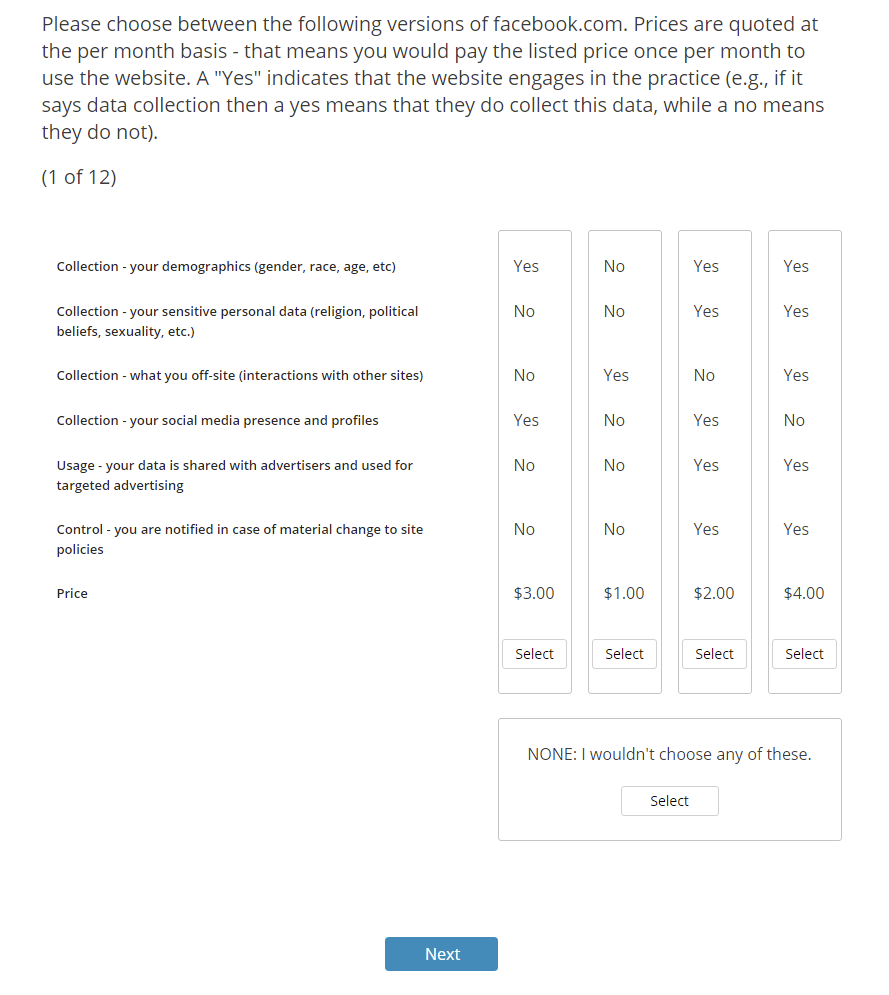
\includegraphics[scale = .5]{manual_figures/survey/conjoint-example-paper.png}
\end{figure}

Two aspects of our design should be noted. First, we implement our conjoint with a specific website in mind, as practitioners have long highlighted the necessity of specific and realistic choice settings for estimate consistency \citep{conjointly_tips_for_setting_up_conjoint_studies}. Second, the literature on conjoint has found that products with many attributes are likely to confuse participants, leading to poor quality data. To overcome this, we follow practitioners and implement a \emph{partial-profile} conjoint design \citep{sawtooth_cbc_partial_profile}. In partial profile designs, a subset of attributes (in our case, six) are chosen at random for each task and vary across products. Price is always included, and non-visible attributes are assumed to be held constant across products within a task. While partial profile designs require more data collection to estimate preferences, they have been shown to generate more reliable data \citep{Chrzan2010PartialProfile}.

To make sure participants understand the choice task, our survey includes multiple examples and attention checks to ensure participants (1) understand how products vary within a task and (2) recognize that non-visible attributes remain constant across all products within a choice task. Next, we estimate specify a hierarchical Bayesian utility model in order to estimate preferences from our conjoint data \citep{rossi2005bayesian}. 

\subsection{Model and Estimation}

Utility for respondent $n$, task $t$, alternative $a$ is:
\begin{align*}
  U_{n,t,a} = 
  \begin{cases}
    \bm x_{n,t,a}^\top \boldsymbol{\beta}_{n} + \alpha_{w(n)} + \boldsymbol{\gamma}^\top \bm d_n + \varepsilon_{n,t,a} & a \in \{1,\dots,A\} \text{ (in-market)} \\[0.3em]
    0 + \varepsilon_{n,t,A+1} & a = A+1 \text{ (outside)}
  \end{cases}
\end{align*}
where $\varepsilon_{n,t,a} \overset{\text{iid}}{\sim} T1EV$, outside utility is fixed at 0 for identification. The utility function has three additive components beyond individual preferences:
\begin{enumerate}[leftmargin=*,nosep]
  \item $\bm x_{n,t,a}^\top \boldsymbol{\beta}_{n}$: Individual-specific feature preferences (hierarchical)
  \item $\alpha_{w(n)}$: Website-specific intercept (random effect)
  \item $\boldsymbol{\gamma}^\top \bm d_n$: Demographic utility shifter (fixed effect)
\end{enumerate}

The website random intercepts ($\alpha_w$) capture website-specific baseline attractiveness that is not explained by the observed features. Some websites may be inherently more engaging or trustworthy, leading respondents to be more likely to choose any alternative when viewing that website's privacy policy. In addition, we include demographic utility shifters ($\boldsymbol{\gamma}$) which are a \emph{utility level shifters} that apply equally to all in-market alternatives. Demographics do not moderate the effects of privacy attributes.

Individual preferences $\boldsymbol{\beta}_{n} \in \mathbb{R}^F$ follow a three-level hierarchy:

\emph{Level 1 (Individual):} 
\begin{align*}
  \boldsymbol{\beta}_{n} \sim \mathcal{N}(\boldsymbol{\mu}_{c(n)}, \boldsymbol{\Sigma}_{c(n)})
\end{align*}
We use non-centered parameterization to improve sampling efficiency:
\begin{align*}
  \boldsymbol{\beta}_{n} = \boldsymbol{\mu}_{c(n)} + \mathbf{L}_{\Sigma_{c(n)}} \bm z_n, \quad \bm z_n \sim \mathcal{N}(\mathbf{0}, \mathbf{I}_F)
\end{align*}

\emph{Level 2 (Website Category):} Covariance decomposition:
\begin{align*}
  \boldsymbol{\Sigma}_c = \text{diag}(\boldsymbol{\tau}_c) \, \boldsymbol{\Omega} \, \text{diag}(\boldsymbol{\tau}_c), \quad \mathbf{L}_{\Sigma_c} = \text{diag}(\boldsymbol{\tau}_c) \mathbf{L}_\Omega
\end{align*}
where:
\begin{align*}
  \boldsymbol{\mu}_c &\sim \mathcal{N}(\mathbf{0}, 5^2 \mathbf{I}_F) \quad \text{(category mean preferences)} \\
  \tau_{c,f} &\sim \text{Lognormal}(0, \sigma_\tau^2) \quad \text{(within-category heterogeneity)}
\end{align*}
with $\sigma_\tau = 0.75$ for privacy and website features ($f = 1, \ldots, 20$), and $\sigma_\tau = 0.5$ for price ($f = 21$).

\emph{Level 3 (Population):} Shared correlation structure:
\begin{align*}
  \mathbf{L}_\Omega \sim \text{LKJcorr}(5), \quad \boldsymbol{\Omega} = \mathbf{L}_\Omega \mathbf{L}_\Omega^\top
\end{align*}

In addition to preference parameters, our model includes website random effects for the individual's preferred website and demographic fixed effects. We complete our model by specifying their hierarchical structure. The website effects follow a hierarchical structure with sum-to-zero constraint:
\begin{align*}
  \alpha_w^{\text{raw}} &\sim \mathcal{N}(0, 1) \quad \forall w \in \{1,\ldots,W\} \\
  \sigma_w &\sim \text{Lognormal}(0, 0.5^2) \\
  \alpha_w &= \sigma_w \cdot \left( \alpha_w^{\text{raw}} - \bar{\alpha}^{\text{raw}} \right)
\end{align*}
where $\bar{\alpha}^{\text{raw}} = \frac{1}{W} \sum_{w=1}^W \alpha_w^{\text{raw}}$. This parameterization ensures $\sum_w \alpha_w = 0$ for identification. Finally, demographic effects have a prior distribution of:
\begin{align*}
  \boldsymbol{\gamma} \sim \mathcal{N}(\mathbf{0}, \mathbf{I}_D)
\end{align*}
this weakly informative prior regularizes toward zero effect, appropriate given small sample sizes in some demographic groups.

\paragraph{Choice probability.} After integrating out T1EV errors, we obtain the multinomial logit:
\begin{align*}
  P(y_{n,t} = a \mid \boldsymbol{\beta}_{n}, \alpha_{w(n)}, \boldsymbol{\gamma}) = \frac{\exp(V_{n,t,a})}{\sum_{k=1}^{A+1} \exp(V_{n,t,k})}
\end{align*}
where:
\begin{align*}
  V_{n,t,a} = \begin{cases} \bm x_{n,t,a}^\top \boldsymbol{\beta}_{n} + \alpha_{w(n)} + \boldsymbol{\gamma}^\top \bm d_n & a \leq A \\ 0 & a = A+1 \end{cases}
\end{align*}

We use the No-U-Turn Sampler (NUTS) with within-chain parallelization via \texttt{reduce\_sum} \citep{hoffman2014nuts} to estimate our model. We run four parallel chains, with 2000 warmup iterations and 3000 sampling iterations per chain.

\newpage
\section{Additional Figures and Tables}


\subsection{Figures on Experimental Sample}

\begin{figure}[H]
\centering
\caption{Demographic Composition of Experimental Sample}\label{fig:dem_balance}

\begin{subfigure}[t]{0.48\textwidth}
  \centering
  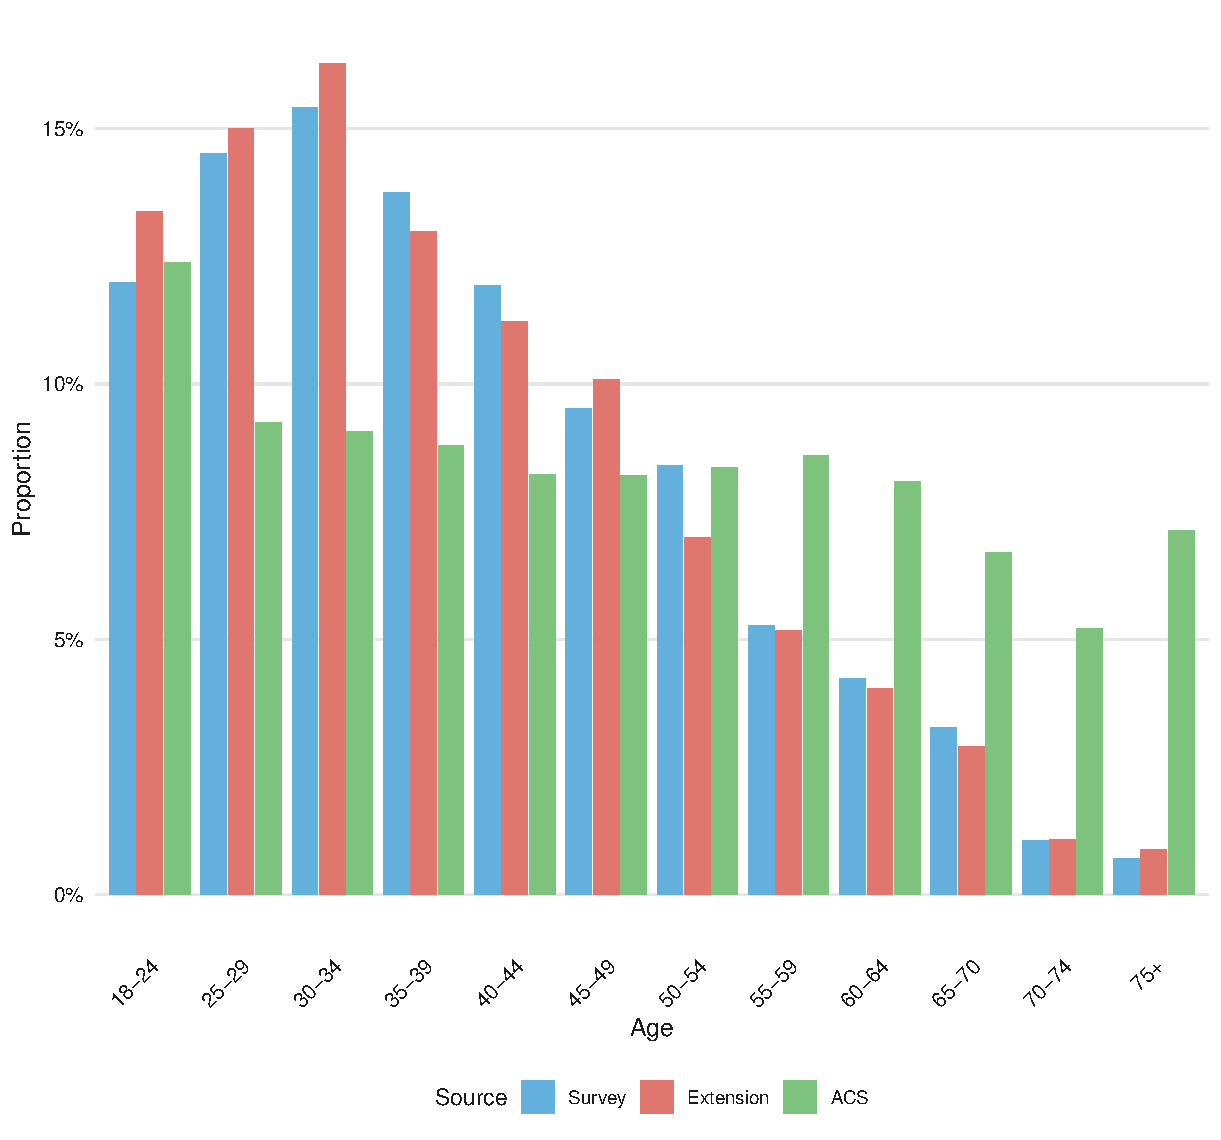
\includegraphics[width=\linewidth]{./output/figures/balance/age.pdf}
  \caption{Age}\label{fig:dem_balance_age}
\end{subfigure}\hfill
\begin{subfigure}[t]{0.48\textwidth}
  \centering
  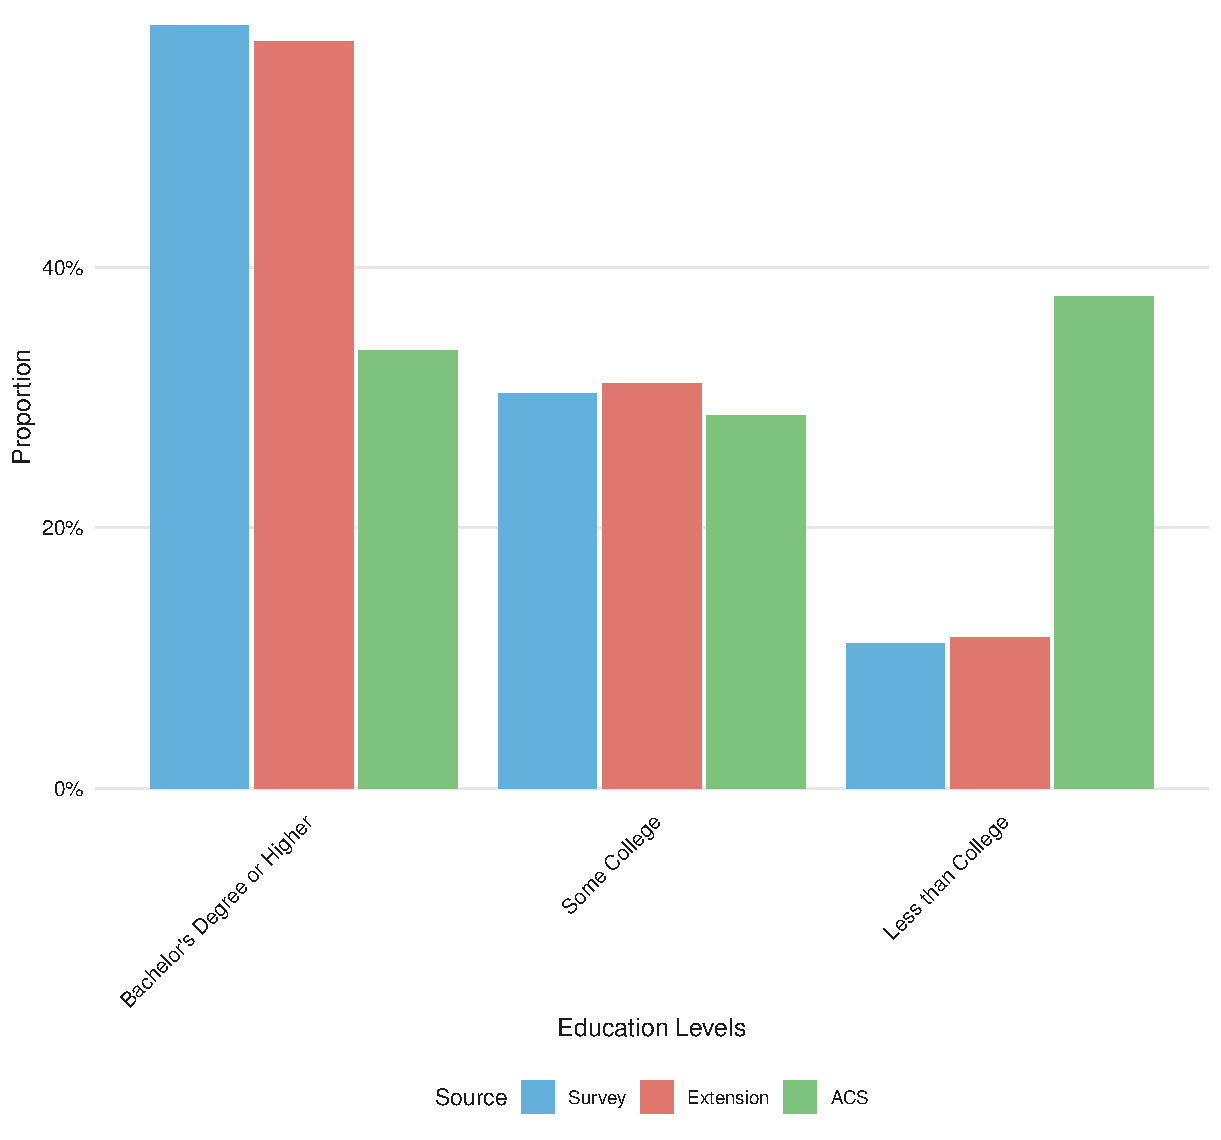
\includegraphics[width=\linewidth]{./output/figures/balance/education.pdf}
  \caption{Education}\label{fig:dem_balance_education}
\end{subfigure}

\vspace{0.6em}

\begin{subfigure}[t]{0.48\textwidth}
  \centering
  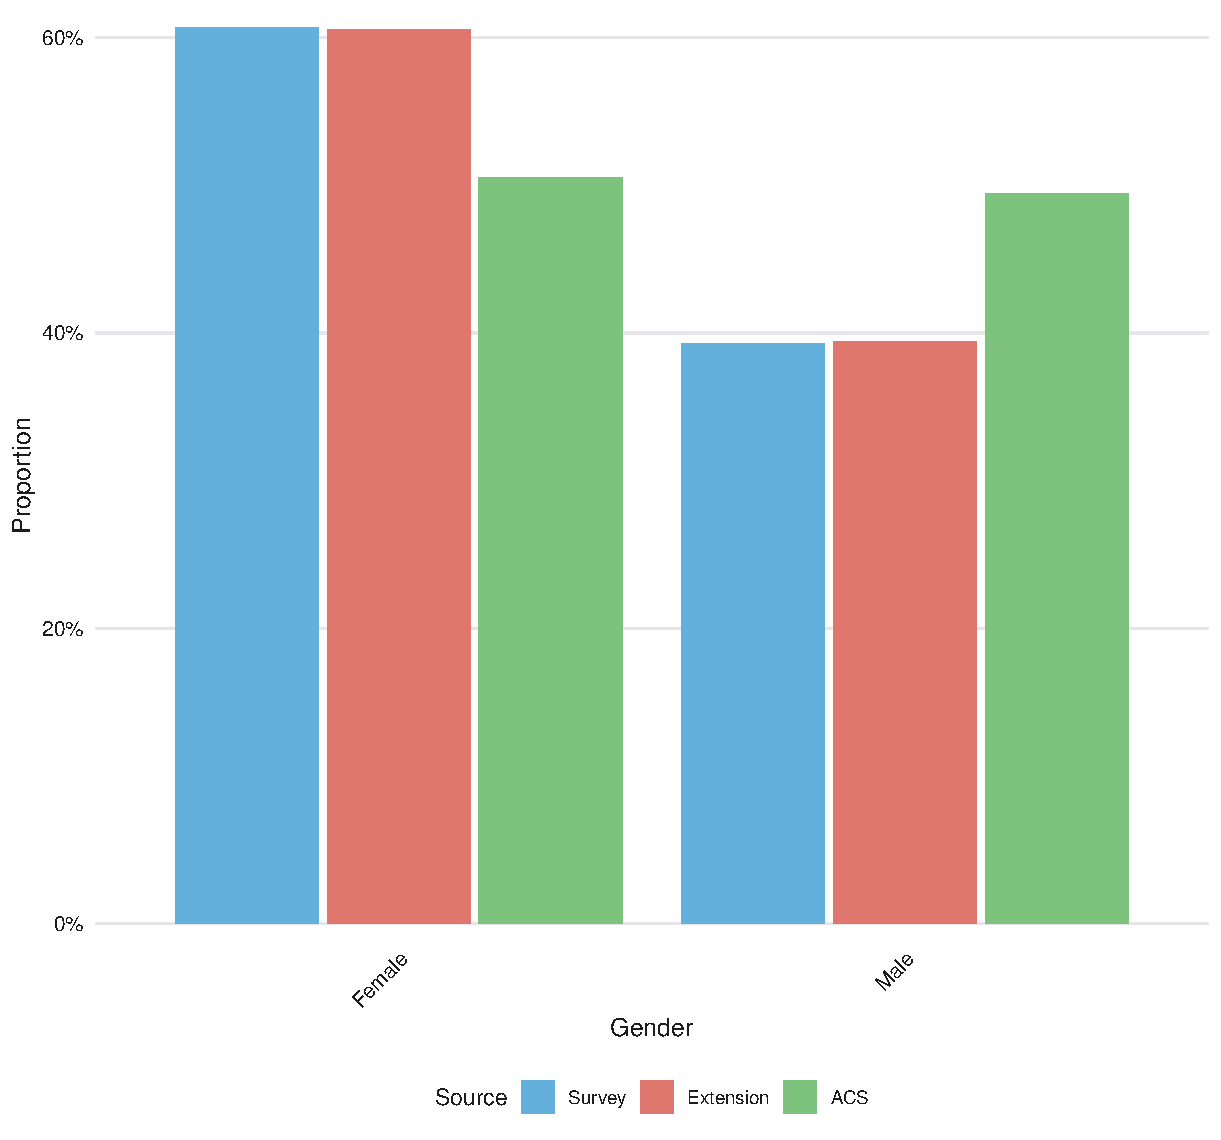
\includegraphics[width=\linewidth]{./output/figures/balance/gender.pdf}
  \caption{Gender}\label{fig:dem_balance_gender}
\end{subfigure}\hfill
\begin{subfigure}[t]{0.48\textwidth}
  \centering
  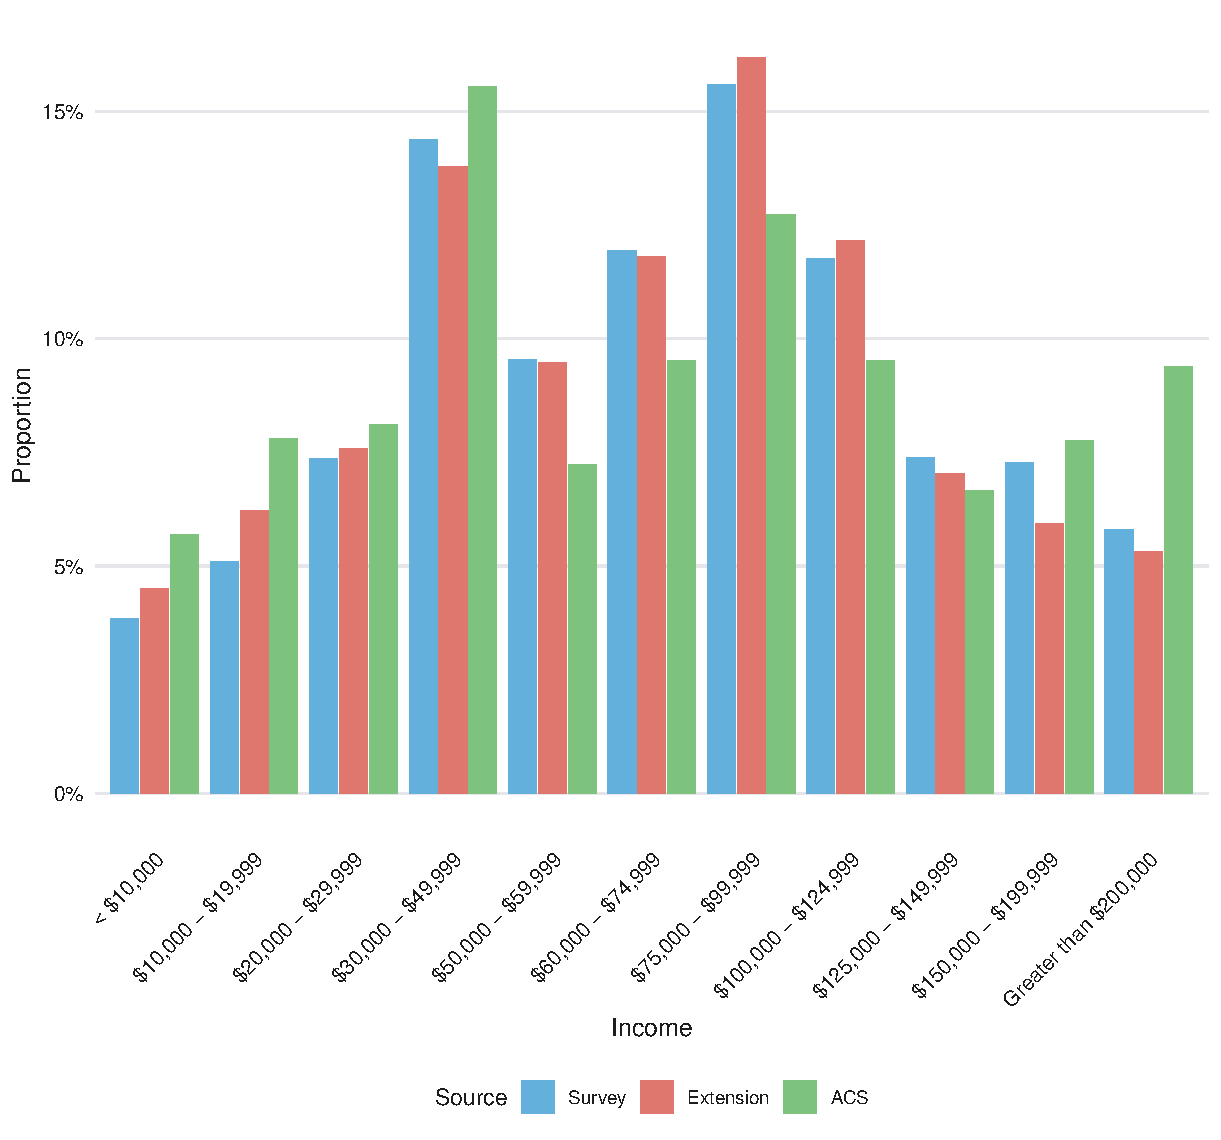
\includegraphics[width=\linewidth]{./output/figures/balance/income.pdf}
  \caption{Income}\label{fig:dem_balance_income}
\end{subfigure}
\caption*{\footnotesize \textsc{Notes}: These figures compare the demographics of the survey sample (blue), extension sample (red), and the 2021 ACS (green) according to age (panel a), education (panel b), gender (panel c), and income (panel d). The survey sample includes all participants who completed the baseline survey. The extension sample conditions on participants who installed the browser extension and were randomized into the experiment. The ACS represents the American Community Survey census estimates from 2021.}
\end{figure}


\begin{table}[H]
\caption{Experimental Balance Tables}\label{tab:exp_balance_table}
\centering
\scalebox{0.8}{
\scalebox{0.8}{
\begin{tabular}{|l|c|c|c|c|c|}
\hline
 & Control Mean & Saliency Mean & Information Mean & p (S vs C) & p (I vs C) \\
\hline
Total Hours on Sites with Privacy Info & 17.906 & 17.747 & 18.103 & 0.918 & 0.900 \\
\hline
Daily Hours on Sites with Privacy Info & 1.279 & 1.268 & 1.293 & 0.918 & 0.900 \\
\hline
Total Hours Spent Online & 28.311 & 28.476 & 28.553 & 0.936 & 0.905 \\
\hline
Male & 0.378 & 0.385 & 0.400 & 0.801 & 0.451 \\
\hline
College Graduate & 0.568 & 0.556 & 0.586 & 0.711 & 0.535 \\
\hline
Age & 38.410 & 38.605 & 39.336 & 0.812 & 0.261 \\
\hline
Income & 80586.374 & 79399.548 & 81011.007 & 0.708 & 0.896 \\
\hline
No Income Disclosure & 0.015 & 0.013 & 0.015 & 0.795 & 1.000 \\
\hline
Is White & 0.761 & 0.767 & 0.763 & 0.829 & 0.943 \\
\hline
Privacy Attitude Index & 0.580 & 0.579 & 0.575 & 0.875 & 0.570 \\
\hline
Privacy Knowledge & 0.914 & 0.910 & 0.908 & 0.829 & 0.747 \\
\hline
PEW Extensive Margin & 0.648 & 0.671 & 0.658 & 0.438 & 0.748 \\
\hline
WTA & 19.000 & 19.200 & 19.049 & 0.698 & 0.927 \\
\hline
Mean Beliefs (Use) & 52.509 & 52.093 & 52.114 & 0.660 & 0.679 \\
\hline
Mean Beliefs (Collect) & 60.741 & 61.016 & 59.586 & 0.802 & 0.290 \\
\hline
Mean Beliefs (Control) & 45.277 & 45.653 & 46.546 & 0.759 & 0.313 \\
\hline
Mean Beliefs (Quality) & 61.607 & 61.983 & 61.278 & 0.764 & 0.804 \\
\hline
Conjoint category (News) & 0.271 & 0.254 & 0.244 & 0.531 & 0.327 \\
\hline
Conjoint category (Entertainment) & 0.246 & 0.250 & 0.235 & 0.887 & 0.667 \\
\hline
Conjoint category (E-commerce) & 0.246 & 0.259 & 0.256 & 0.622 & 0.724 \\
\hline
Conjoint category (Social) & 0.237 & 0.237 & 0.265 & 1.000 & 0.289 \\
\hline
\end{tabular}
}


}
\caption*{\scriptsize \textsc{Notes}: This table presents the experimental balance table computed at the time of randomization. The columns denote the mean in the control, saliency, and information groups respectively with the final two columns denoting the p-value between the saliency and control as well as the information and control, respectively. The rows are as follows: total hours on sites with privacy information during baseline, daily hours on sites with privacy information during baseline (can differ due to differences in entry period), total hours spent online during baseline, male fraction, fraction with at least a college degree, age, income, choosing to not disclose income, fraction of participants that are white, privacy attitude index (combining PEW questions on privacy attitudes), privacy knowledge question regarding the ability of websites to track consumers across time without an email address, PEW question on likelihood of stopping to use a website based on privacy concerns, extension WTA, mean beliefs for prevalence of use/collect/control/quality attributes, and the fraction whose conjoint category is news/entertainment/e-commerce/social.}
\end{table}


\begin{table}[H]
\caption{Top Websites used by Participants}
\label{tab:top_websites}
\resizebox{\textwidth}{!}{
\begin{tabular}{rlrrr}
  \hline
 & Domain & Daily Hours (per Active User) & Number of Users & Daily Hours (over all users) \\ 
  \hline
1 & \topWebOneDomain{} & \topWebOneActiveHours{} & \topWebOneNUsers{} & \topWebOneAllHours{} \\ 
  2 & \topWebTwoDomain{} & \topWebTwoActiveHours{} & \topWebTwoNUsers{} & \topWebTwoAllHours{} \\ 
  3 & \topWebThreeDomain{} & \topWebThreeActiveHours{} & \topWebThreeNUsers{} & \topWebThreeAllHours{} \\ 
  4 & \topWebFourDomain{} & \topWebFourActiveHours{} & \topWebFourNUsers{} & \topWebFourAllHours{} \\ 
  5 & \topWebFiveDomain{} & \topWebFiveActiveHours{} & \topWebFiveNUsers{} & \topWebFiveAllHours{} \\ 
  6 & \topWebSixDomain{} & \topWebSixActiveHours{} & \topWebSixNUsers{} & \topWebSixAllHours{} \\ 
  7 & \topWebSevenDomain{} & \topWebSevenActiveHours{} & \topWebSevenNUsers{} & \topWebSevenAllHours{} \\ 
  8 & \topWebEightDomain{} & \topWebEightActiveHours{} & \topWebEightNUsers{} & \topWebEightAllHours{} \\ 
  9 & \topWebNineDomain{} & \topWebNineActiveHours{} & \topWebNineNUsers{} & \topWebNineAllHours{} \\ 
  10 & \topWebTenDomain{} & \topWebTenActiveHours{} & \topWebTenNUsers{} & \topWebTenAllHours{} \\ 
  11 & \topWebElevenDomain{} & \topWebElevenActiveHours{} & \topWebElevenNUsers{} & \topWebElevenAllHours{} \\ 
  12 & \topWebTwelveDomain{} & \topWebTwelveActiveHours{} & \topWebTwelveNUsers{} & \topWebTwelveAllHours{} \\ 
  13 & \topWebThirteenDomain{} & \topWebThirteenActiveHours{} & \topWebThirteenNUsers{} & \topWebThirteenAllHours{} \\ 
  14 & \topWebFourteenDomain{} & \topWebFourteenActiveHours{} & \topWebFourteenNUsers{} & \topWebFourteenAllHours{} \\ 
  15 & \topWebFifteenDomain{} & \topWebFifteenActiveHours{} & \topWebFifteenNUsers{} & \topWebFifteenAllHours{} \\ 
   \hline
\end{tabular}
}
\caption*{\footnotesize \textsc{Notes}: This table presents the top 15 websites used in our sample with the domain, the daily hours per active user, the number of users and the daily hours including non-users. All statistics are computed using the baseline period.}
\end{table}

\begin{figure}[H]
\caption{Privacy Preferences and Beliefs across (Exogenous) Survey Payment}
\label{fig:selection_on_survey_payments}
\begin{center}
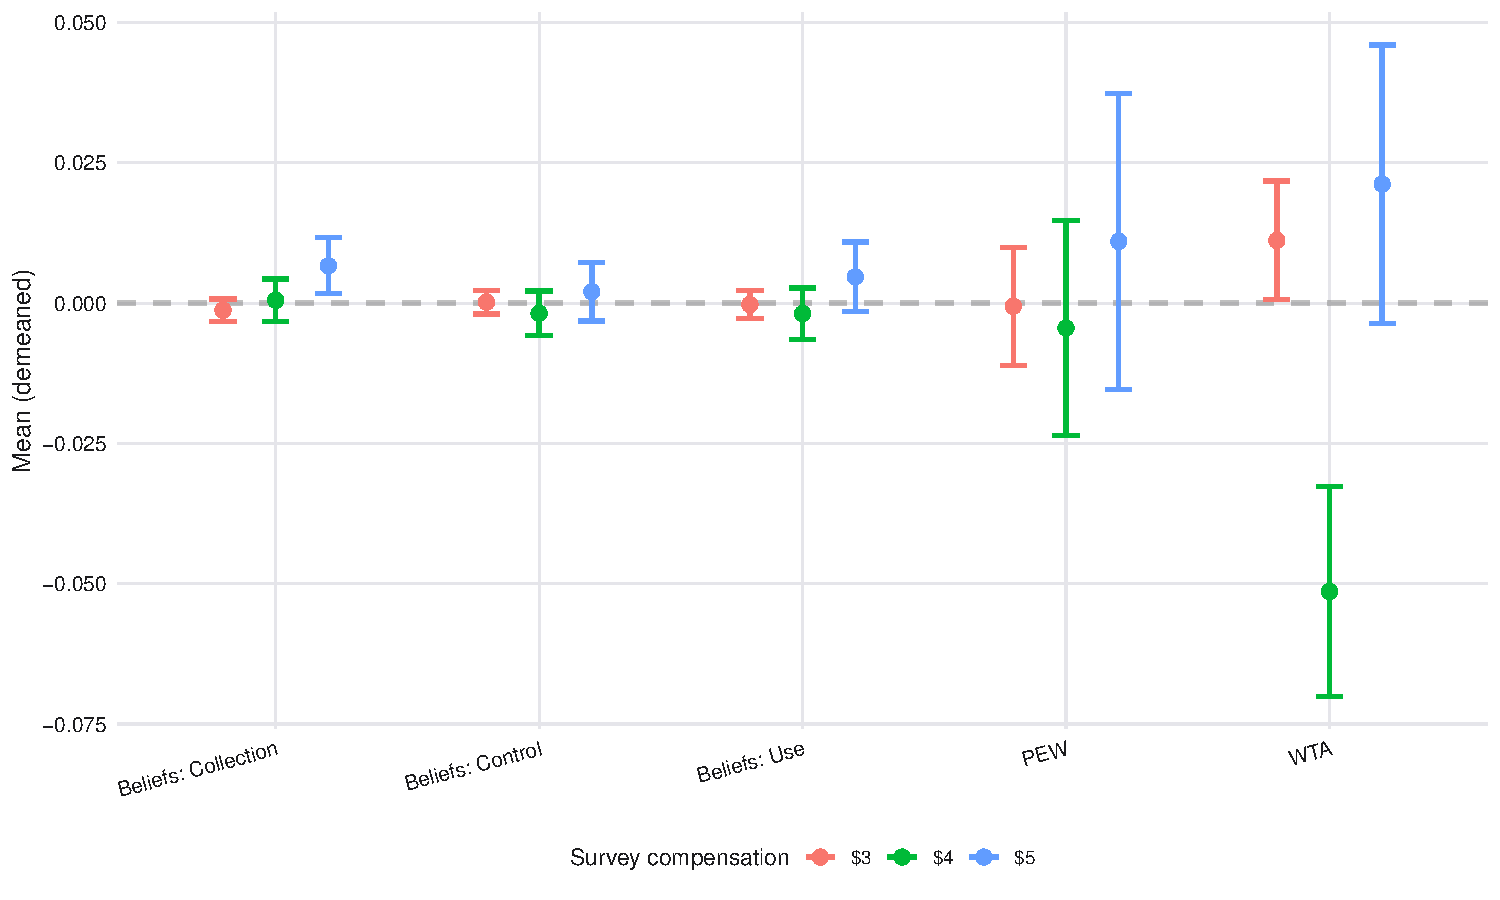
\includegraphics[scale=0.4]{./output/figures/agg_selection_lots.pdf}
\end{center}
\caption*{\scriptsize \textsc{Notes}: This figure presents a comparison across the random survey offers presented to the experimental participants (\$3, \$4, \$5). From left to right, we compare degree of belief misspecification for collection attributes, control attributes, use attributes, an index of the PEW questions, and the extension WTA. Bars represent 95\% confidence intervals.}
\end{figure}

\begin{figure}[H]
\begin{center}
\caption{PEW Comparison}\label{fig:pew_comparison}
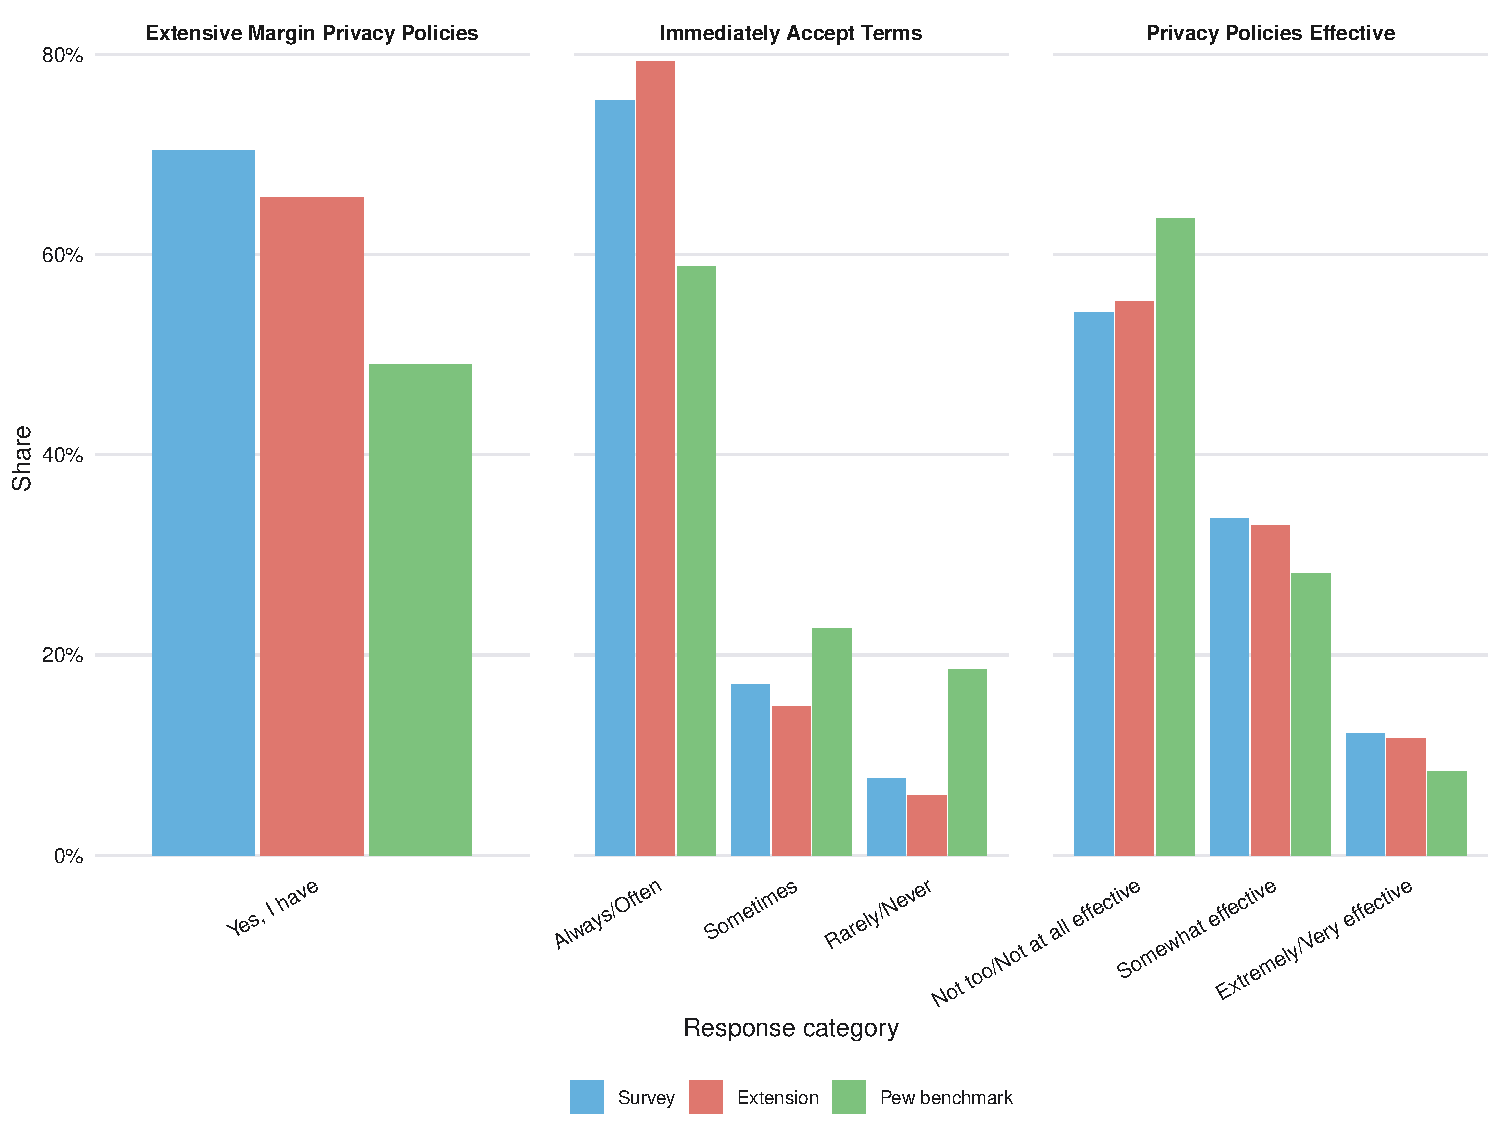
\includegraphics[scale=0.4]{./output/figures/pew_comparison.pdf}
\end{center}
\caption*{\scriptsize \textsc{Notes}: This figure compares the PEW values across the (i) sample of participants who completed the survey (denoted survey sample, blue), (ii) sample of participants who were in the extension subsample (red), and (iii) the values from PEW (green). The question in the left panel  measures the fraction of participants who have ever stopped using a website due to privacy concerns. The question in the center panel measures how often participants self-report clicking ``agree'' right away without reading the contents of the privacy terms. The question in the right panel measures how effective the participants believe privacy policies are as a way for companies to communicate how they are using people's data. The content of the questions can be found in \url{https://www.pewresearch.org/wp-content/uploads/sites/20/2023/10/PI_2023.10.18_Data-Privacy_TOPLINE-1.pdf}.}
\end{figure}

\begin{table}[H] \centering 
\caption{Changes in Experimental Behavior}\label{tab:experimenter_demand}
\scalebox{0.9}{

\begingroup
\centering
\begin{tabular}{lcc}
   \tabularnewline \midrule \midrule
                         & Disrupted Browsing & Evaded Extension/Chrome \\   
   Model:                & (1)                & (2)\\  
   \midrule
   \emph{Variables}\\
   Constant              & 0.028$^{***}$      & 0.021$^{***}$\\   
                         & (0.009)            & (0.006)\\   
   Saliency Treatment    & 0.096$^{***}$      & 0.017$^{**}$\\   
                         & (0.013)            & (0.008)\\   
   Information Treatment & 0.113$^{***}$      & 0.024$^{***}$\\   
                         & (0.013)            & (0.008)\\   
   \midrule
   \emph{Fit statistics}\\
   Observations          & 1,334              & 1,334\\  
   R$^2$                 & 0.06416            & 0.00727\\  
   Adjusted R$^2$        & 0.06275            & 0.00578\\  
   \midrule \midrule
   \multicolumn{3}{l}{\emph{IID standard-errors in parentheses}}\\
   \multicolumn{3}{l}{\emph{Signif. Codes: ***: 0.01, **: 0.05, *: 0.1}}\\
\end{tabular}
\par\endgroup



}
\caption*{\scriptsize \textsc{Notes}: This table presents the differences in self-reported changes in behavior due to the extension installation. We estimate OLS regressing the dependent variable on treatment status. Column (1) reports differences to the following question: ``How much did the experiment disturb your normal
online browsing?" on a scale from 0 (Not at all) to 1 (Always) in increments of 0.25. Column (2) reports differences to the following question: ``Did you take any actions to evade the browser extension? (e.g. browse more on your phone, or on a different browser)" on a scale from 0 (Not at all) to 1 (Always) in increments of 0.25.}
\end{table}


\begin{figure}[H]
\caption{Privacy Valuations between Extension and Survey Sample}
\label{fig:extension_survey_conjoint_sample}
\begin{center}
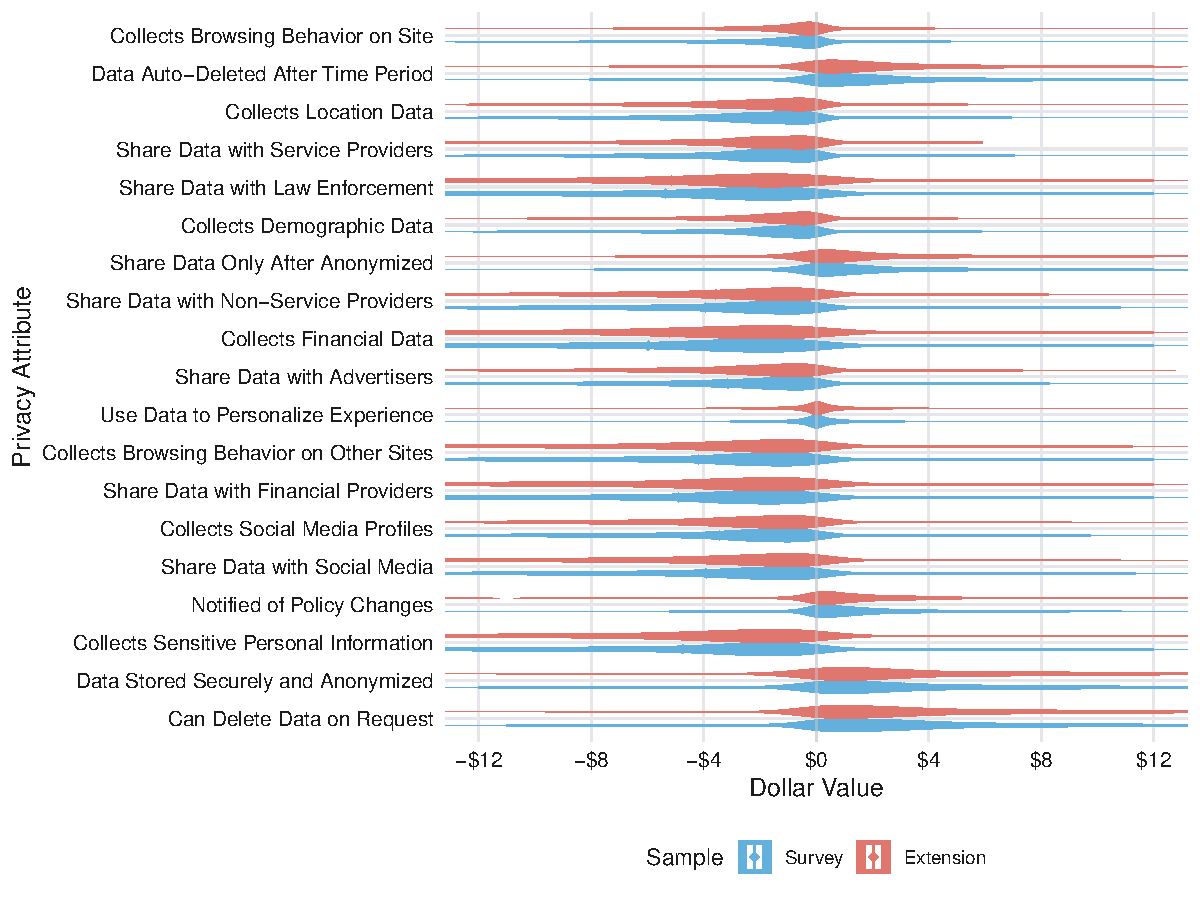
\includegraphics[scale=0.6]{./output/figures/individual_heterogeneity_experiment_vs_survey.pdf}
\end{center}
\caption*{\scriptsize \textsc{Notes}: This figure presents a comparison of the estimated monthly willingness to pay for the different privacy attributes between the survey sample (blue) and extension sample (red).}
\end{figure}

\begin{figure}[H]
\centering
\caption{Privacy Valuations and Most Valued Information (Full Sample)}
\label{fig:privacy_combined_full}

\begin{subfigure}[t]{\textwidth}
    \centering
    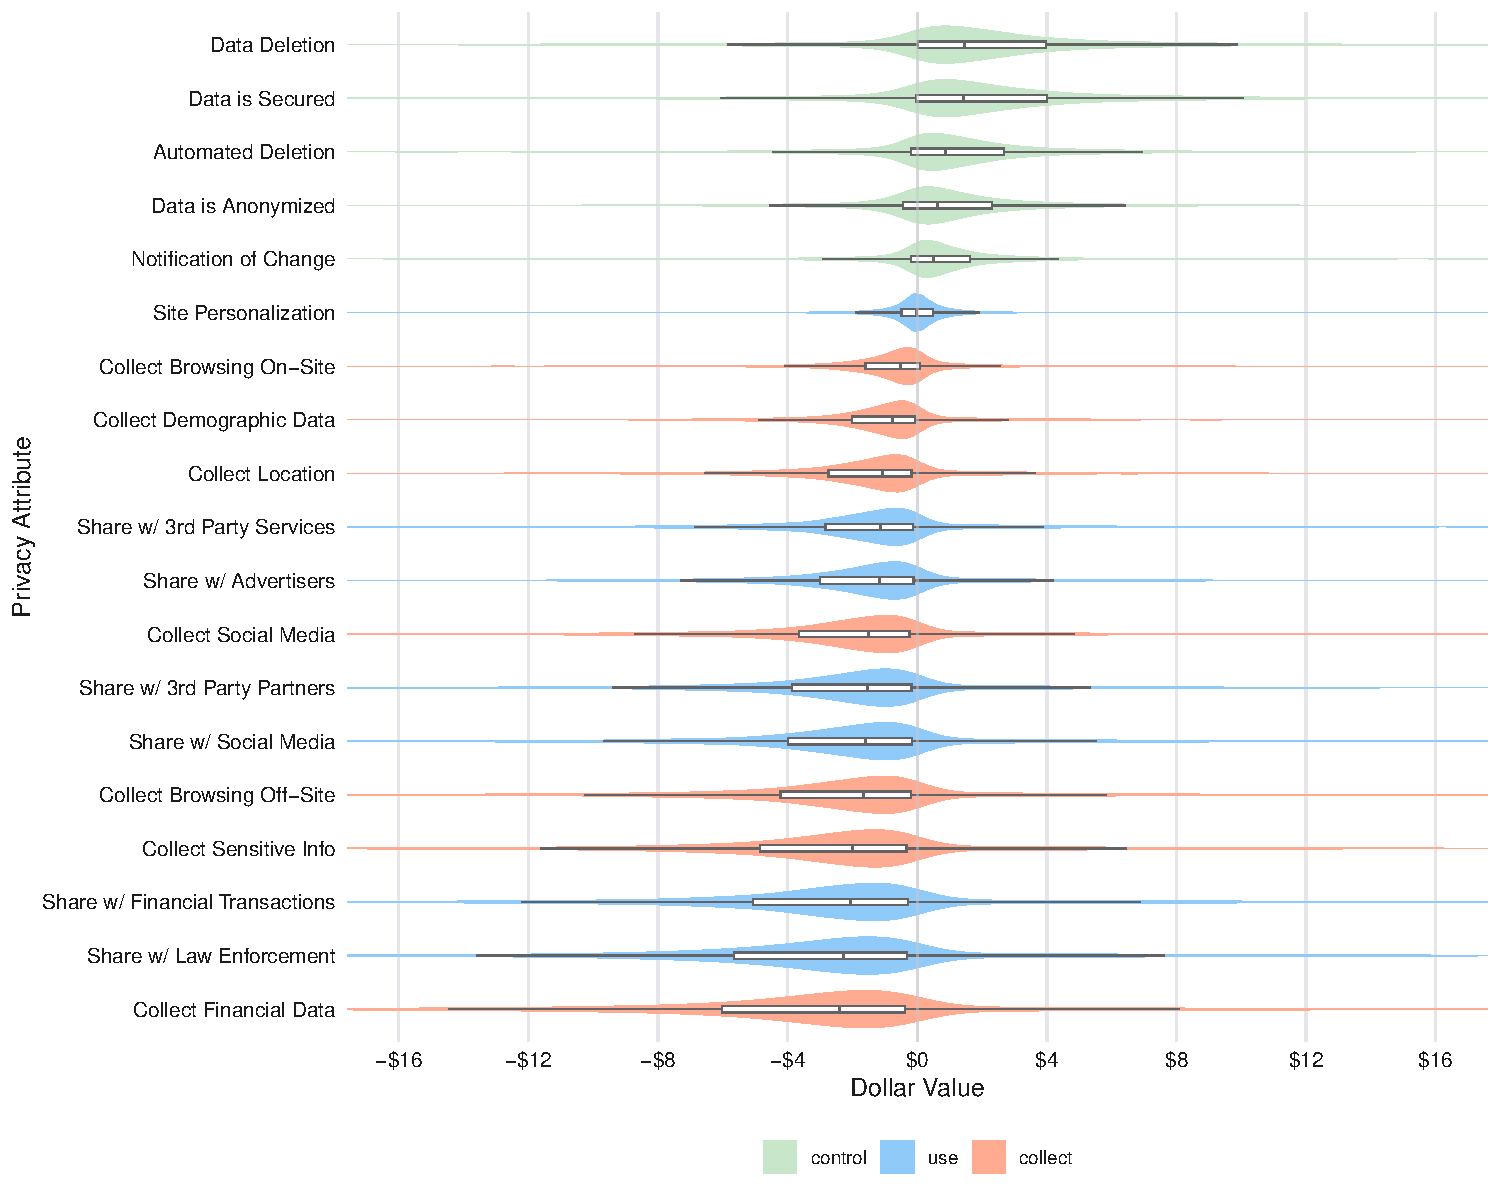
\includegraphics[width=0.7\textwidth]{./output/figures/individual_heterogeneity_dollars_with_website_full.pdf}
    \caption{WTP for Privacy Attributes}
    \label{fig:privacy_info_partworth_full}
\end{subfigure}
\begin{subfigure}[t]{0.7\textwidth}
    \centering
    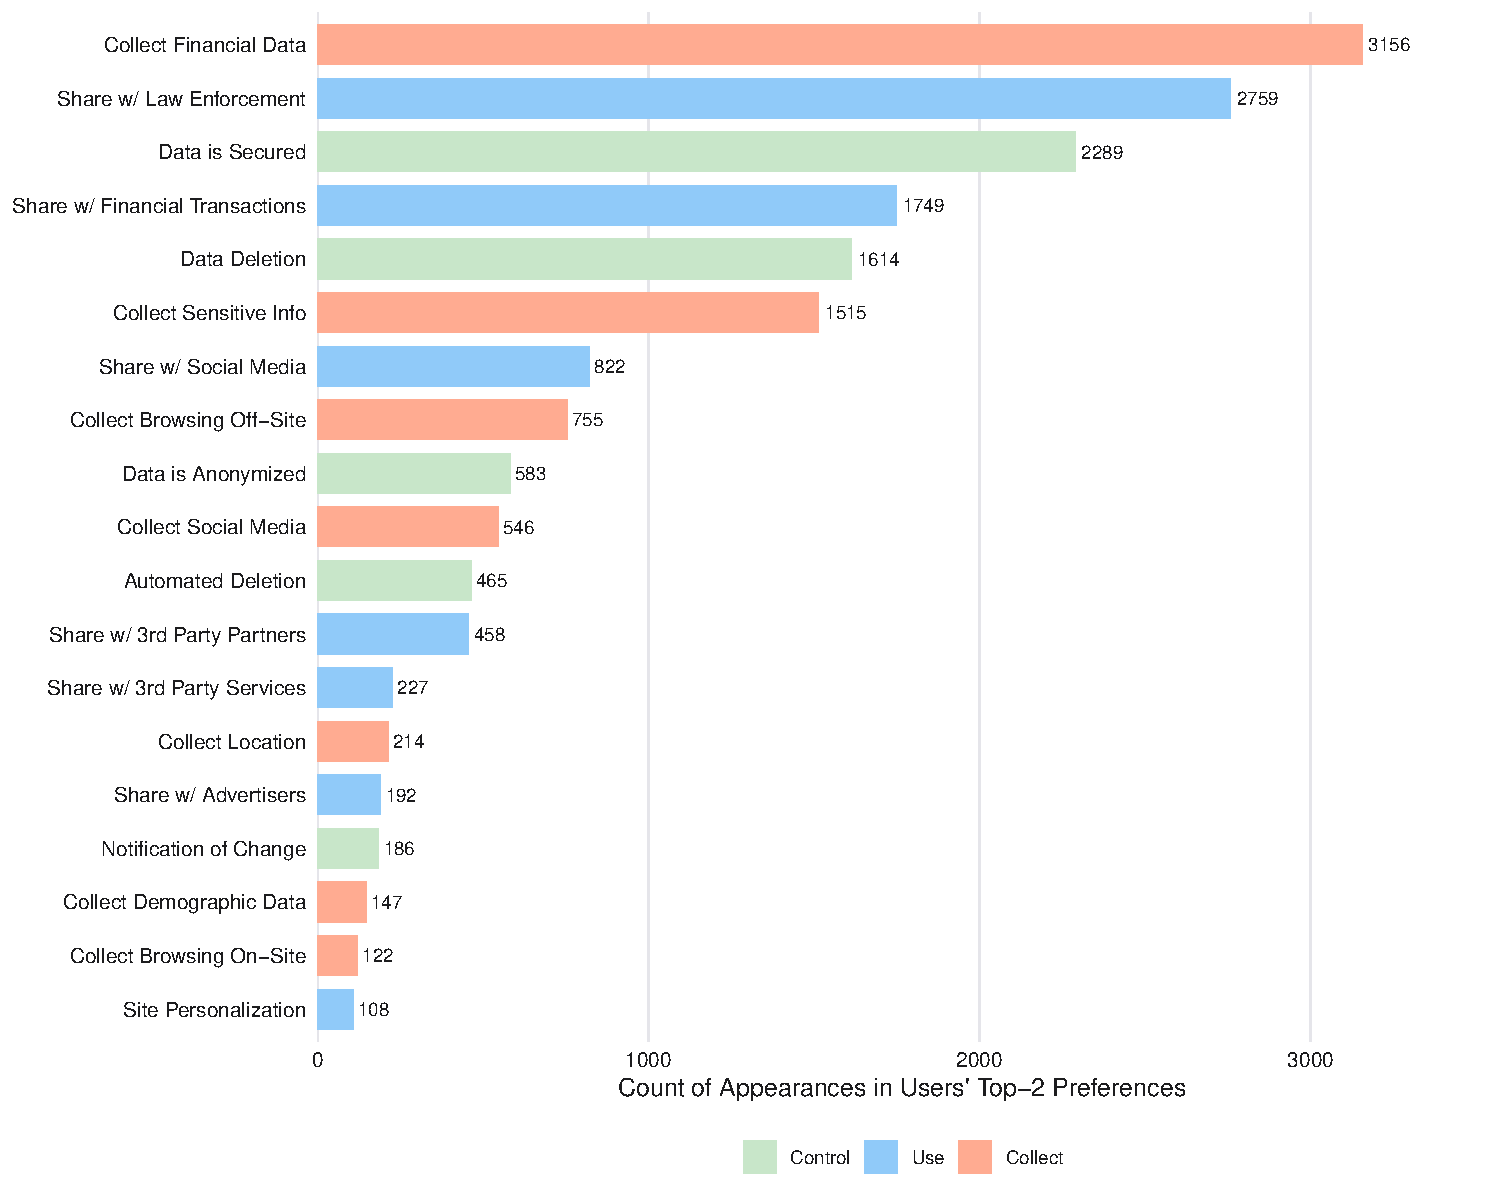
\includegraphics[width=\textwidth]{./output/figures/top2_privacy_attributes_full.pdf}
    \caption{Most Valued Information}
    \label{fig:privacy_info_top_2_full}
\end{subfigure}

\vspace{0.4em}
\caption*{\scriptsize \textsc{Notes}: Both panels use the full conjoint sample, including all respondents who completed the baseline survey. Panel (a) presents the estimated monthly willingness to pay for different privacy attributes, computed using the estimated part-worth for each attribute and the price coefficient. Green rows denote ``Control'' attributes, blue rows denote ``Use'' attributes, and orange rows denote ``Collect'' attributes. Panel (b) shows the distribution of top-2 personalized attributes. Information value is computed per Equation \eqref{eq:provided_info}. The extension sample versions are in Figures \ref{fig:privacy_combined} (WTP) and \ref{fig:privacy_info_top_2} (top-2 attributes).}
\end{figure}

\begin{figure}[H]
\centering
\caption{Most Valued Information: Top-2 Personalized Attributes}
\label{fig:privacy_info_top_2}
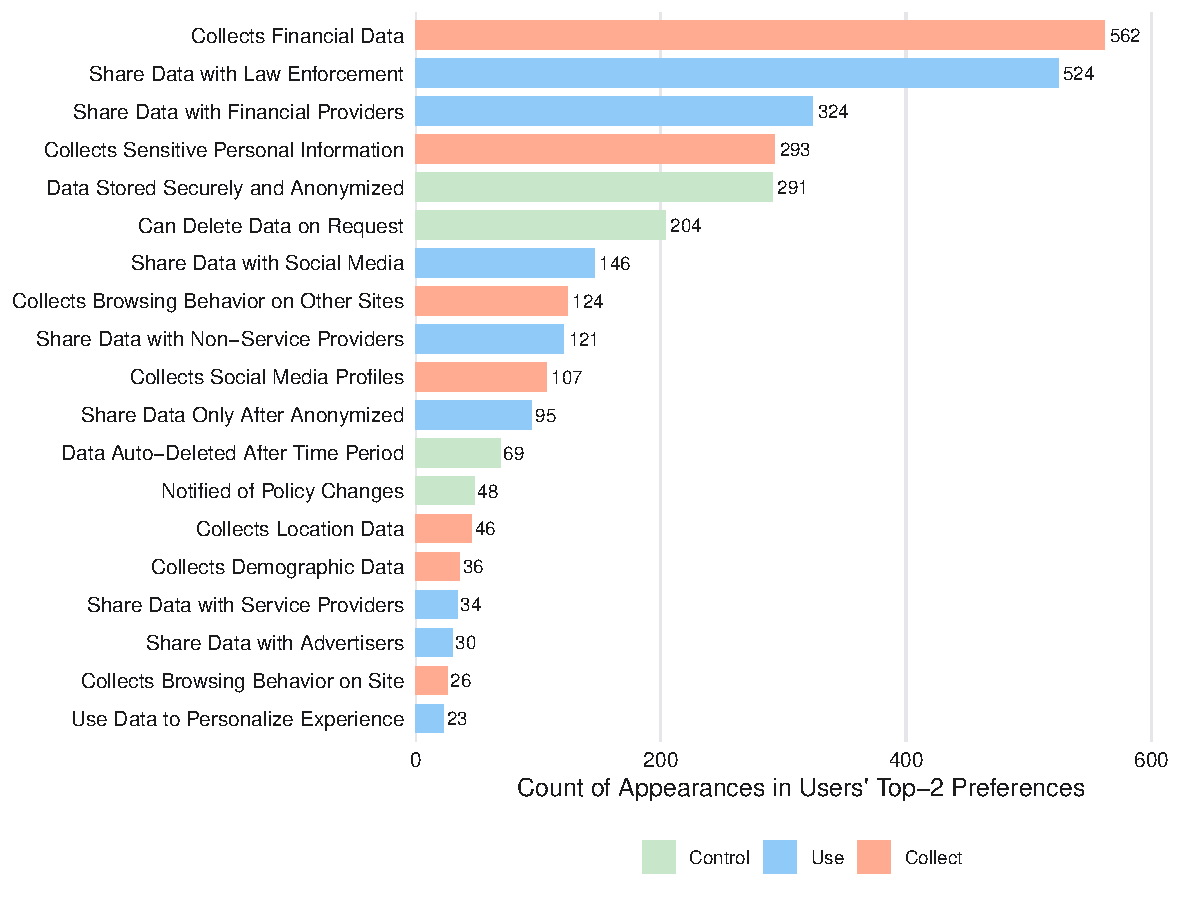
\includegraphics[width=0.62\textwidth]{./output/figures/top2_privacy_attributes_extension.pdf}
\vspace{0.4em}
\caption*{\scriptsize \textsc{Notes}: Distribution of the top-2 personalized attributes across participants in the extension sample. Information value is computed per Equation \eqref{eq:provided_info}. The full conjoint sample version appears in Figure \ref{fig:privacy_combined_full} (panel b).}
\end{figure}

\begin{table}[H]
   \caption{Belief Misspecification and Privacy Preference Intensity}\label{tab:conjoint_vs_beliefs}
   \centering
   
\begin{table}[htbp]
   \caption{Belief Misspecification and Privacy Preference Intensity}
   \centering
   \begin{tabular}{lccc}
      \tabularnewline \midrule \midrule
      Dependent Variable: & \multicolumn{3}{c}{Part-Worth (Aligned)}\\
                            & Discrete      & Linear                  & Over/Under \\   
      Model:                & (1)           & (2)                     & (3)\\  
      \midrule
      \emph{Variables}\\
      Underestimate         & 0.016$^{***}$ &                         &   \\   
                            & (0.002)       &                         &   \\   
      Overestimate          & -0.005$^{*}$  &                         &   \\   
                            & (0.003)       &                         &   \\   
      Misspecification (pp) &               & -0.0001$^{**}$          &   \\   
                            &               & ($5.05\times 10^{-5}$)  &   \\   
      Overestimate (pp)     &               &                         & $9.29\times 10^{-5}$\\    
                            &               &                         & ($7.53\times 10^{-5}$)\\    
      Underestimate (pp)    &               &                         & -0.0003$^{***}$\\   
                            &               &                         & ($5.55\times 10^{-5}$)\\    
      \midrule
      \emph{Fixed-effects}\\
      Attribute FE          & Yes           & Yes                     & Yes\\  
      Participant FE        & Yes           & Yes                     & Yes\\  
      \midrule
      \emph{Fit statistics}\\
      Observations          & 141,094       & 141,094                 & 141,094\\  
      R$^2$                 & 0.59353       & 0.59335                 & 0.59342\\  
      Within R$^2$          & 0.00057       & 0.00011                 & 0.00029\\  
      \midrule \midrule
      \multicolumn{4}{l}{\emph{Clustered (Participant FE) standard-errors in parentheses}}\\
      \multicolumn{4}{l}{\emph{Signif. Codes: ***: 0.01, **: 0.05, *: 0.1}}\\
   \end{tabular}
\end{table}



   \caption*{\scriptsize \textsc{Notes}: This table estimates the relationship between belief misspecification and privacy preference intensity. The dependent variable is the aligned part-worth, where positive values indicate stronger preferences to avoid the privacy practice. Misspecification is defined as the participant's belief (scaled 0--100) minus the ground truth prevalence (0--100). Column (1) uses discrete indicators for underestimation and overestimation relative to the rounded ground truth, with correct beliefs as the omitted category. Column (2) uses continuous misspecification in percentage points. Column (3) separates misspecification into overestimation and underestimation components. All specifications include attribute and participant fixed effects with standard errors clustered at the participant level.}
\end{table}



\begin{table}[H]
   \caption{Demographic Heterogeneity in Belief Misspecification and Preferences}\label{tab:baseline_demo_heterogeneity}
   \centering
   
\begin{table}[htbp]
   \caption{Demographic Heterogeneity in Belief Misspecification and Preferences}
   \centering
   \begin{tabular}{lcc}
      \tabularnewline \midrule \midrule
      Dependent Variables:                & |Misspecification| (pp) & Part-Worth (Aligned)\\  
                                          &                         & Preferences \\   
      Model:                              & (1)                     & (2)\\  
      \midrule
      \emph{Variables}\\
      Age 30--44                          & -0.0951                 & 0.0018\\   
                                          & (0.1791)                & (0.0074)\\   
      Age 45--59                          & -0.0086                 & 0.0024\\   
                                          & (0.2045)                & (0.0087)\\   
      Age 60+                             & 0.3283                  & 0.0229$^{**}$\\   
                                          & (0.2677)                & (0.0116)\\   
      Bachelor's Degree or Above          & -0.9529$^{***}$         & 0.0132$^{**}$\\   
                                          & (0.1500)                & (0.0064)\\   
      Household Income $\geq$ \$75k       & -0.2298                 & -0.0071\\   
                                          & (0.1482)                & (0.0063)\\   
      Female                              & 0.0742                  & 0.0566$^{***}$\\   
                                          & (0.1437)                & (0.0063)\\   
      Other/Prefer Not to Answer (Gender) & -0.8945                 & 0.1083$^{***}$\\   
                                          & (0.5895)                & (0.0281)\\   
      \midrule
      \emph{Fixed-effects}\\
      Attribute FE                        & Yes                     & Yes\\  
      \midrule
      \emph{Fit statistics}\\
      Observations                        & 139,232                 & 138,130\\  
      R$^2$                               & 0.21708                 & 0.23605\\  
      Within R$^2$                        & 0.00071                 & 0.00628\\  
      \midrule \midrule
      \multicolumn{3}{l}{\emph{Clustered (Participant FE) standard-errors in parentheses}}\\
      \multicolumn{3}{l}{\emph{Signif. Codes: ***: 0.01, **: 0.05, *: 0.1}}\\
   \end{tabular}
\end{table}



   \caption*{\scriptsize \textsc{Notes}: This table estimates demographic heterogeneity in belief misspecification and privacy preferences. Column (1) regresses absolute belief misspecification (in percentage points) on demographic covariates. Column (2) regresses the aligned part-worth on the same covariates. The omitted categories are age 18--29, no bachelor's degree, household income below \$75k, and male. All specifications include attribute fixed effects with standard errors clustered at the participant level.}
\end{table}



\subsection{Figures for Belief Updating and Search}
\begin{figure}[H]
\begin{center}
\caption{Heterogeneity based on (Ex Ante) Exposure - Tercile}\label{fig:top_sites_heterogeneity_exposure}
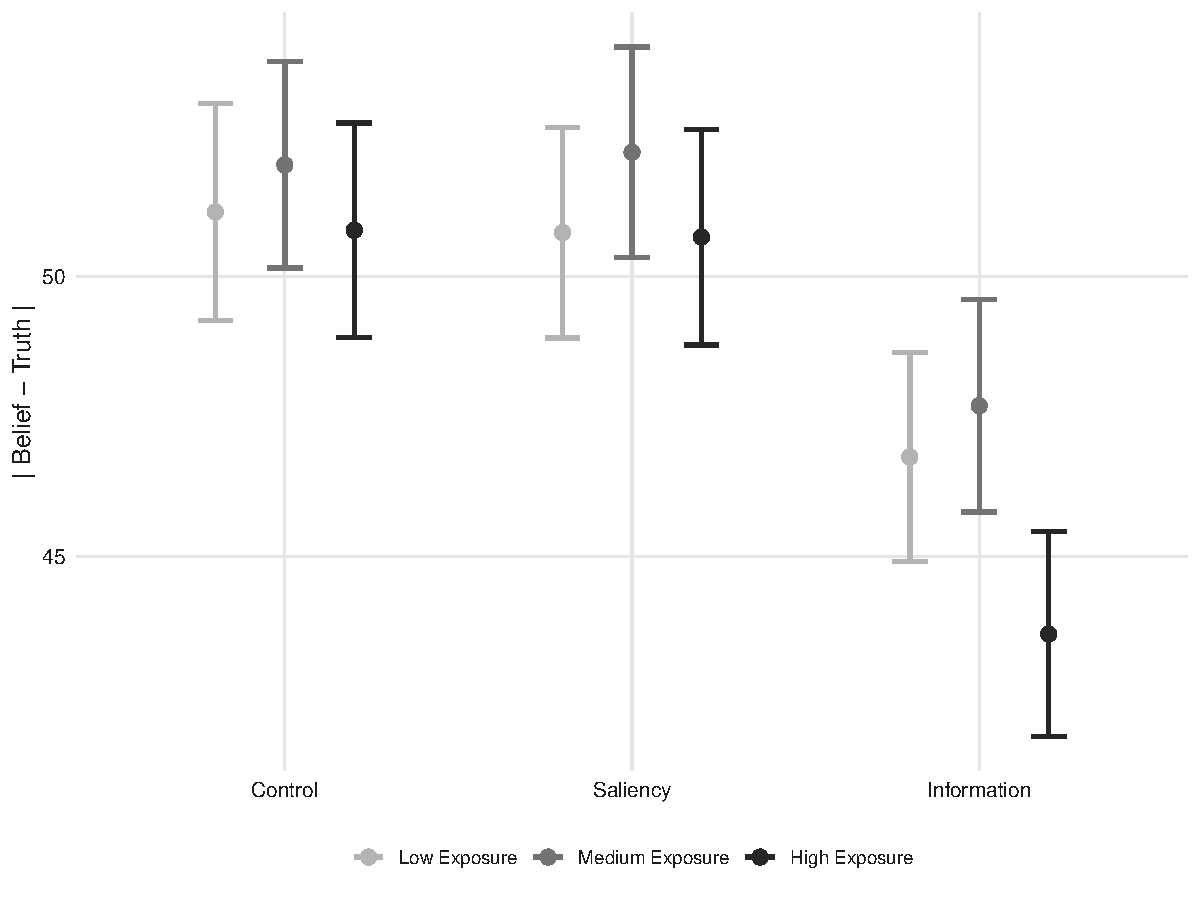
\includegraphics[scale=0.5]{./output/figures/heterogeneous_beliefs_site_level_by_exposure_tercile.pdf}
\end{center}
\caption*{\scriptsize \textsc{Notes}: This figure presents the differences in beliefs about the most preferred privacy attributes in the endline survey compared to the ground truth. For each experimental group, we partition each (website, participant) tuple into terciles based on the time spent in the baseline period. We then plot the mean and associated 95\% confidence interval for the estimate for each tercile and experimental group.}
\end{figure}

\begin{table}[htbp]
   \caption{Belief Correctness on Top Sites -- Random Information}\label{tab:belief_correctness_top_sitesrandom_info}
   \centering
   \scalebox{0.9}{
   \begin{tabular}{lccc}
   \tabularnewline \midrule \midrule
                         & $\lvert \text{Belief} - \text{Truth} \rvert$     & Correctness (Weak) & Correctness (Strict) \\   
   Model:                & (1)                                              & (2)                & (3)\\  
   \midrule
   \emph{Variables}\\
   Saliency Treatment    & 1.52                                             & -0.035             & -0.023\\   
                         & (1.53)                                           & (0.024)            & (0.020)\\   
   Information Treatment & -3.44$^{**}$                                     & 0.050$^{**}$       & 0.054$^{***}$\\   
                         & (1.46)                                           & (0.023)            & (0.019)\\   
   \midrule
   \emph{Fixed-effects}\\
   Website FE            & Yes                                              & Yes                & Yes\\  
   Block FE              & Yes                                              & Yes                & Yes\\  
   \midrule
   \emph{Fit statistics}\\
   Observations          & 5,772                                            & 4,580              & 5,772\\  
   R$^2$                 & 0.21843                                          & 0.25693            & 0.20070\\  
   Within R$^2$          & 0.00345                                          & 0.00506            & 0.00434\\  
   \midrule \midrule
   \multicolumn{4}{l}{\emph{Clustered (experiment\_id) standard-errors in parentheses}}\\
   \multicolumn{4}{l}{\emph{Signif. Codes: ***: 0.01, **: 0.05, *: 0.1}}\\
\end{tabular}

   }
   \caption*{\scriptsize \textsc{Notes}: OLS estimates from Equation (3). Includes website, attribute, and randomization block fixed effects. Column (1): Dependent variable is $|\text{Belief}_{ijk} - \text{Truth}_{jk}|$, where beliefs are scaled to $\{0, 25, 50, 75, 100\}$ and truth is binary $\{0, 100\}$. Column (2): Binary indicator equal to 1 if response is correct, excluding neutral responses of 50. Column (3): Strict correctness, equal to 1 if $(\text{Belief} > 50) = (\text{Truth} = 100)$. The beliefs are the likelihood of the website engaging in the specified privacy practice for the top 5 most visited sites during the intervention and a random attribute that is not in the top 2 most informative attributes according to Equation \eqref{eq:provided_info}.}
\end{table}
\begin{figure}[H]
\caption{CDF of Belief Correctness}\label{fig:cdf_belief_correctness_top_sites}
\begin{center}
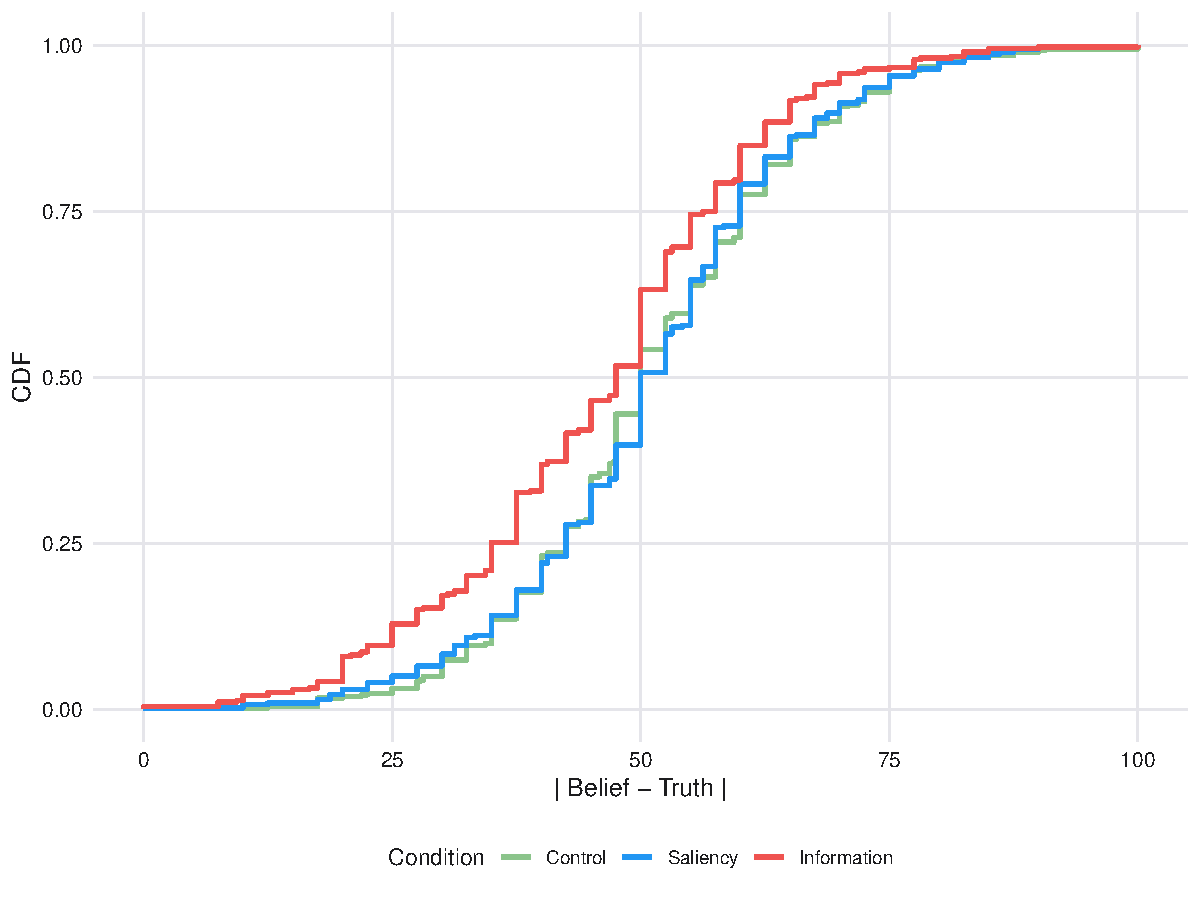
\includegraphics[scale=0.5]{./output/figures/cumulative_belief_distance.pdf}
\end{center}
\caption*{\scriptsize \textsc{Notes}: This presents the CDF of belief correctness of the participant's belief regarding the website engaging in the specified privacy practice for the top 5 most visited sites during the intervention and that is in the top 2 most informative attributes according to Equation \eqref{eq:provided_info}. For each participant we take the average across the two attributes and then compute the CDF across participants within each treatment group.}
\end{figure}

\begin{table}[H]
\caption{Treatment Effect on Cookie Banner Interactions}\label{tab:cookie_banner_interactions_treatment}
\centering
\scalebox{0.9}{

\begin{table}[htbp]
   \caption{Treatment Effect on Cookie Banner Interactions}
   \centering
   \begin{tabular}{lcc}
      \tabularnewline \midrule \midrule
                                   & Cookie Banner Total Interactions & Cookie Banner Distinct Domains \\   
      Model:                       & (1)                              & (2)\\  
      \midrule
      \emph{Variables}\\
      Saliency Treatment x Post    & 0.416                            & 0.170$^{*}$\\   
                                   & (0.491)                          & (0.088)\\   
      Information Treatment x Post & 0.111                            & 0.056\\   
                                   & (0.508)                          & (0.091)\\   
      \midrule
      \emph{Fixed-effects}\\
      Weeks FE                     & Yes                              & Yes\\  
      Participant FE               & Yes                              & Yes\\  
      Block FE                     & Yes                              & Yes\\  
      \midrule
      \emph{Fit statistics}\\
      Observations                 & 9,576                            & 9,576\\  
      R$^2$                        & 0.55336                          & 0.59043\\  
      Within R$^2$                 & 0.00024                          & 0.00051\\  
      \midrule \midrule
      \multicolumn{3}{l}{\emph{Clustered (Participant FE) standard-errors in parentheses}}\\
      \multicolumn{3}{l}{\emph{Signif. Codes: ***: 0.01, **: 0.05, *: 0.1}}\\
   \end{tabular}
\end{table}



}
\caption*{\scriptsize \textsc{Notes}: This table reports the estimated average treatment effects on engagement with a cookie banner. Engagements with a cookie banner were logged in the analytics system of our extension when a participant would mouse over the cookie banner. Column (1) presents the estimates using the dependent variable of the total number of cookie banner interactions and Column (2) presents the estimates using the dependent variable of the unique number of domains with at least one cookie banner interaction. The data is a balanced panel at the (site, participant) level across weeks. The difference-in-difference equation \eqref{eq:did_search} is estimated for this dependent variable and estimates are clustered at the participant level.}
\end{table}


\subsection{Results on Changes in Behavior}


\begin{table}[H]
\centering
\caption{Data Sharing Purposes}\label{tab:data_sharing_purpose}
\begin{tabular}{lrrl}
  \hline
Consequence & Participants & Percentage & Category \\ 
  \hline
Loss of data control & \dataPurposeLossControlN{} & \dataPurposeLossControlPct{} & Negative \\ 
  Personalized content & \dataPurposePersonalizedN{} & \dataPurposePersonalizedPct{} & Positive \\ 
  More annoying ads & \dataPurposeAnnoyingAdsN{} & \dataPurposeAnnoyingAdsPct{} & Negative \\ 
  Identity theft & \dataPurposeIdentityTheftN{} & \dataPurposeIdentityTheftPct{} & Negative \\ 
  Hacking & \dataPurposeHackingN{} & \dataPurposeHackingPct{} & Negative \\ 
  Better search results & \dataPurposeBetterSearchN{} & \dataPurposeBetterSearchPct{} & Positive \\ 
  Easier sharing/logins & \dataPurposeEasierSharingN{} & \dataPurposeEasierSharingPct{} & Positive \\ 
  Cyberstalking & \dataPurposeCyberstalkingN{} & \dataPurposeCyberstalkingPct{} & Negative \\ 
  Improved services & \dataPurposeImprovedServicesN{} & \dataPurposeImprovedServicesPct{} & Positive \\ 
  Coupons/discounts & \dataPurposeCouponsN{} & \dataPurposeCouponsPct{} & Positive \\ 
  More interesting ads & \dataPurposeInterestingAdsN{} & \dataPurposeInterestingAdsPct{} & Positive \\ 
   \hline
\end{tabular}
\caption*{\scriptsize \textsc{Notes}: Participants were asked to select the 3-5 most important consequences of data sharing online. The table presents the consequence, the number of participants who included it in their top 3-5 most important consequences and the overall percentage of participants that represents, followed by whether it is a positive or negative consequence.}
\end{table}

\begin{table}[H] 
\caption{Treatment Effect on Self-Reported Data Sharing Behavior}\label{tab:treatment_effect_data_sharing}
\scalebox{0.9}{
\begin{tabular}{lcccc}
   \tabularnewline \midrule \midrule
                         & Deleted Cookies & Opted out   & Withheld data & Changed privacy settings \\   
   Model:                & (1)             & (2)         & (3)           & (4)\\  
   \midrule
   \emph{Variables}\\
   Saliency Treatment    & 0.008           & 0.030       & 0.040         & 0.034\\   
                         & (0.040)         & (0.041)     & (0.041)       & (0.039)\\   
   Information Treatment & 0.018           & 0.069$^{*}$ & 0.032         & 0.017\\   
                         & (0.039)         & (0.040)     & (0.039)       & (0.038)\\   
   \midrule
   \emph{Fixed-effects}\\
   Block FE              & Yes             & Yes         & Yes           & Yes\\  
   \midrule
   \emph{Fit statistics}\\
   Observations          & 966             & 966         & 966           & 966\\  
   R$^2$                 & 0.32814         & 0.34462     & 0.34334       & 0.35358\\  
   Within R$^2$          & 0.00036         & 0.00495     & 0.00192       & 0.00129\\  
   \midrule \midrule
   \multicolumn{5}{l}{\emph{Clustered (experiment\_id) standard-errors in parentheses}}\\
   \multicolumn{5}{l}{\emph{Signif. Codes: ***: 0.01, **: 0.05, *: 0.1}}\\
\end{tabular}

}
\caption*{\scriptsize \textsc{Notes}: This table reports the estimated average treatment effects on self-reported changes in data sharing behavior from the endline survey. The first column measures whether a participant self-reports deleting cookies on at least one website or at least once during the intervention period. The second column measures whether a participant self-reports explicitly opting out data sharing with at least one website. The third column measures whether a participant self-reports deciding not to share data with at least one website. The fourth column measures whether a participant self-reports changing privacy settings for at least one website. The data is only available for participants who went through the second wave of the study. We estimate OLS with block-by-wave fixed effects and standard errors clustered at the participant level.}
\end{table}


\begin{comment}
\begin{table}[H] 
\caption{Treatment Effects on Privacy Settings Visits}\label{tab:privacy_settings_visits}
\scalebox{0.9}{
\begin{tabular}{lccc}
   \midrule \midrule
                                                 & Number of Visits & Ever Visit & Distinct Domains \\
   Model:                                        & (1)              & (2)        & (3)\\  
   \midrule
   Saliency Treatment $\times$ Post   & -0.0122  & -0.0019               & -0.0009\\   
                                                             & (0.0154) & (0.0075)              & (0.0079)\\   
   Information Treatment $\times$ Post       & -0.0009  & 0.0014                & 0.0014\\   
                                                             & (0.0126) & (0.0076)              & (0.0079)\\   
   \midrule
   \emph{Fixed-effects}\\
   Weeks FE                     & Yes      & Yes                   & Yes\\  
   Participant FE                                             & Yes      & Yes                   & Yes\\  
   Block FE                                          & Yes      & Yes                   & Yes\\  
   \midrule \midrule
   \multicolumn{4}{l}{\textit{Clustered participant standard-errors in parentheses}}\\
   \multicolumn{4}{l}{\textit{Signif. Codes: ***: 0.01, **: 0.05, *: 0.1}}\\
\end{tabular}
}
\caption*{\scriptsize \textsc{Notes}: This table reports the estimated average treatment effects on visiting privacy settings pages. Engagements with a privacy setting were logged by classification according to the browser history of the participant. Column (1) presents the estimates using the dependent variable of the total number of interactions, Column (2) presents the estimates using the dependent variable of whether they ever visited the privacy policy, and Column (3) presents the estimates using the dependent variable of the distinct number of domains where the participant interacted with the privacy settings. The data is a balanced panel at the (site, participant) level across weeks. The difference-in-difference equation \eqref{eq:did_search} is estimated for this dependent variable and estimates are clustered at the participant level.}
\end{table}
\end{comment}
\subsection{Experimental Design Figures}\label{sec:exp_design_figs}

\begin{figure}[H]
  \caption{Additional Information Dialogs}
\label{fig:additional_experimental_info}
  \centering
  \begin{subfigure}[b]{1.0\linewidth}
    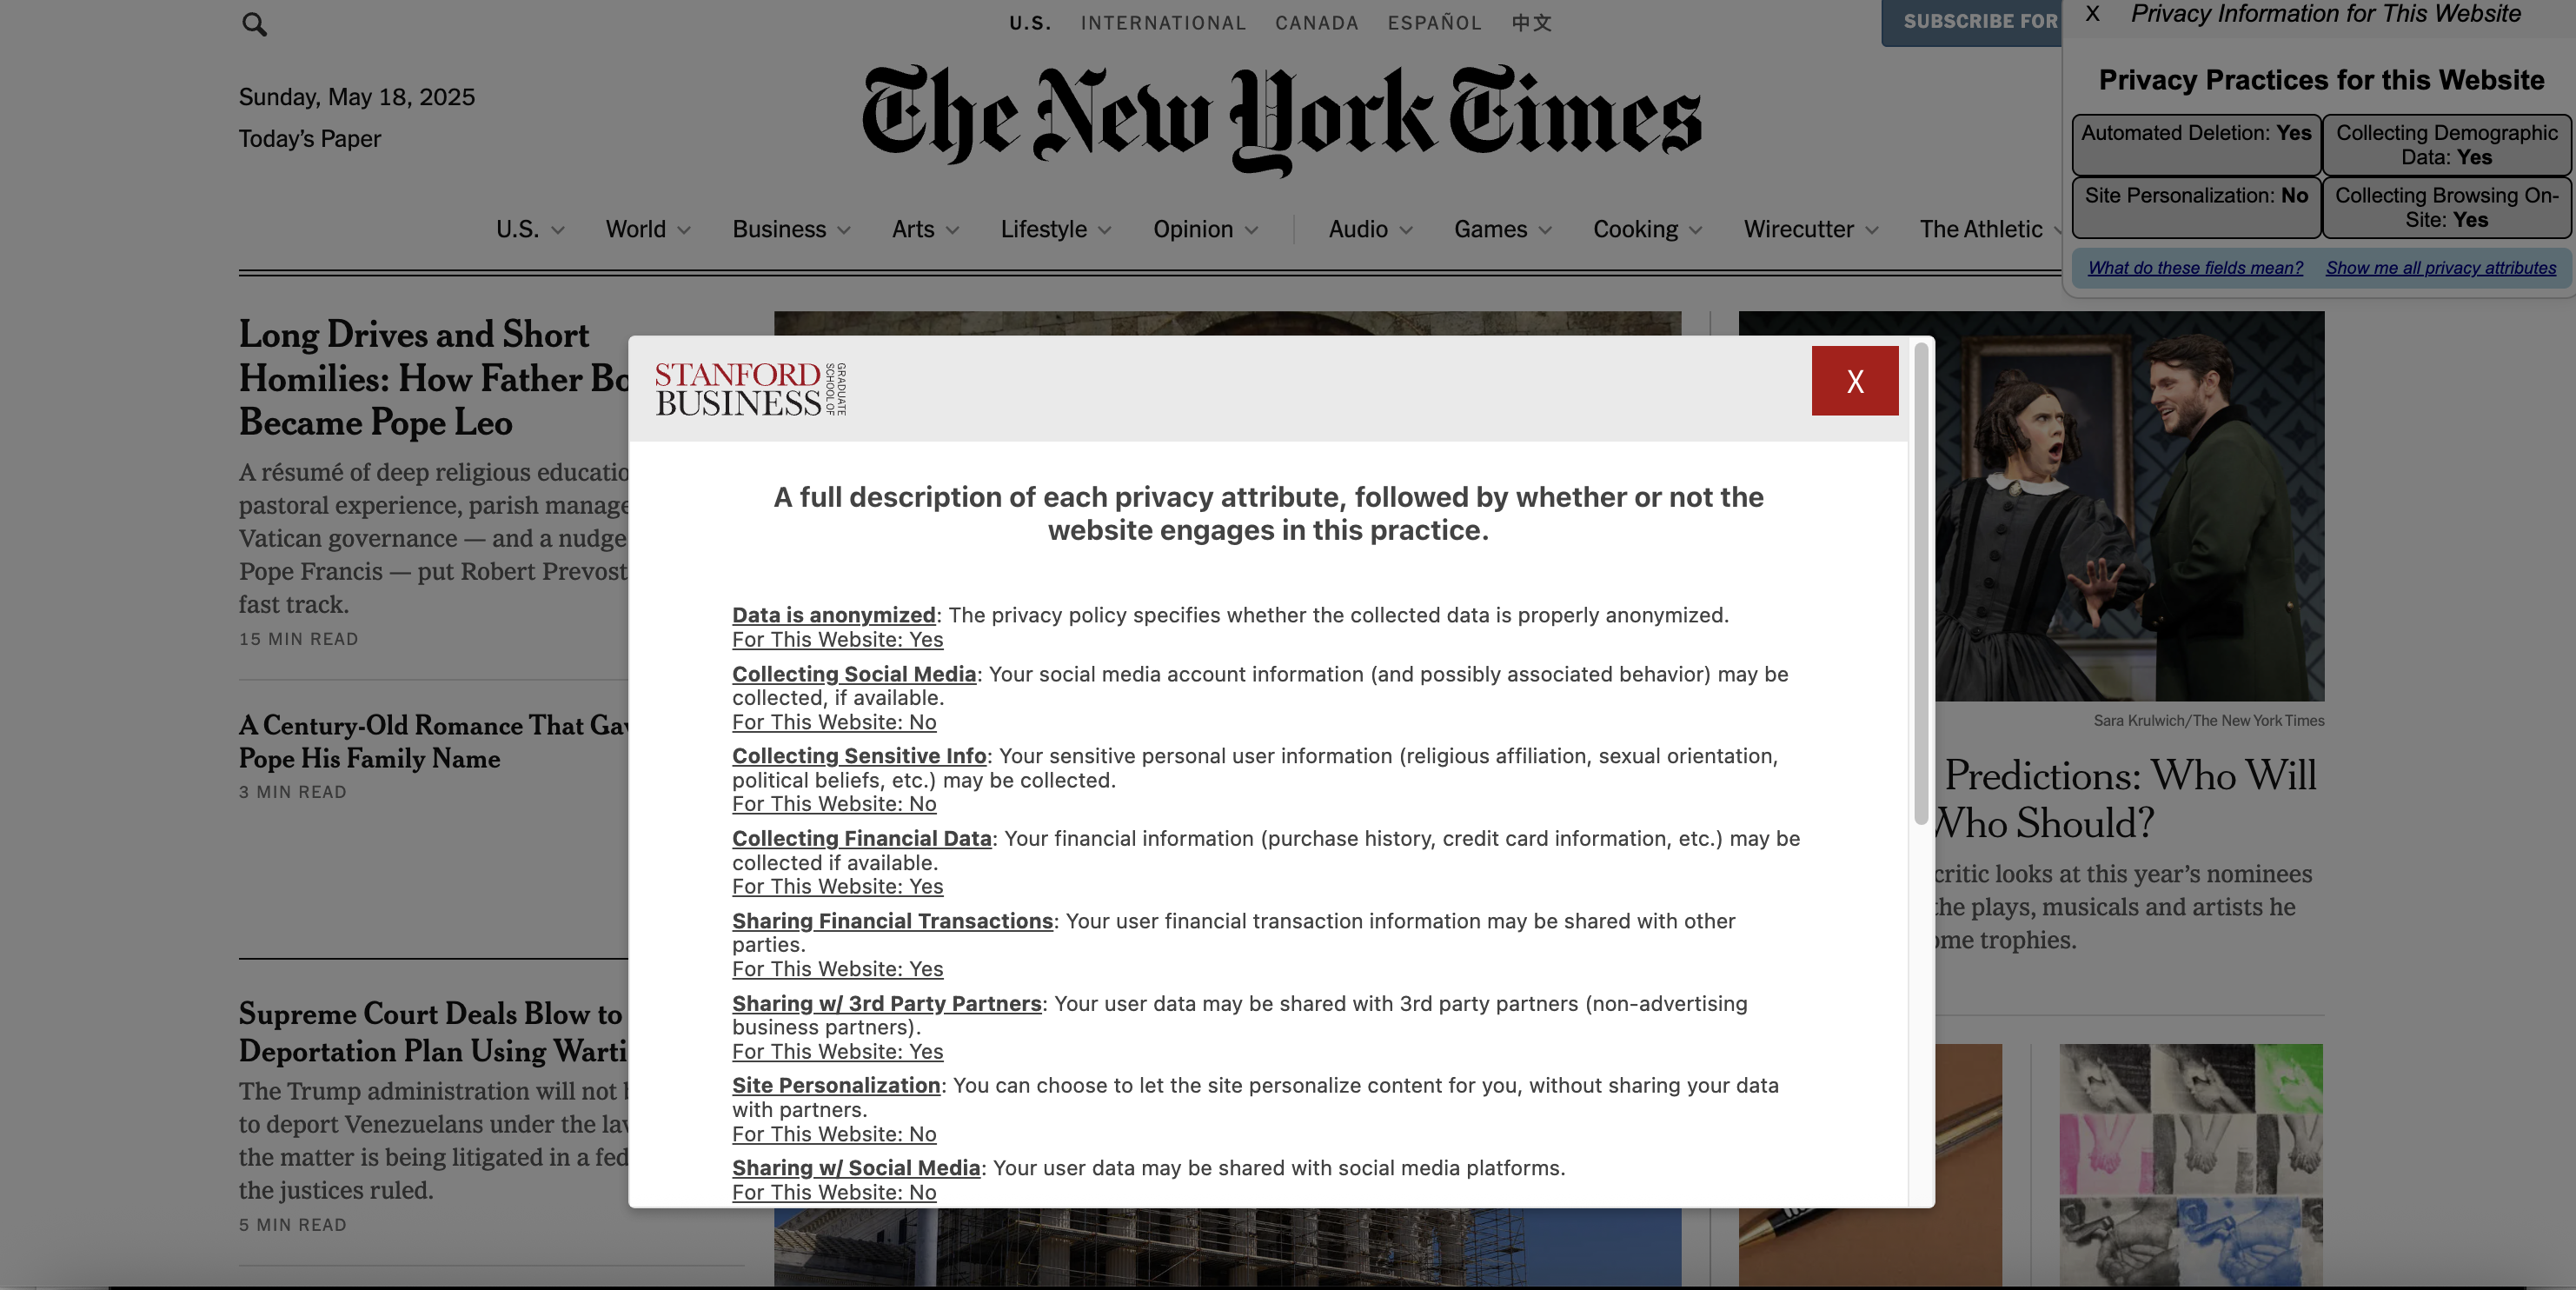
\includegraphics[width=\linewidth]{manual_figures/dialog/info_full_attributes_dialog.png}
    \caption{Full Information}
    \label{fig:attribute_info}
  \end{subfigure}

  \vskip\baselineskip

  \begin{subfigure}[b]{1.0\linewidth}
    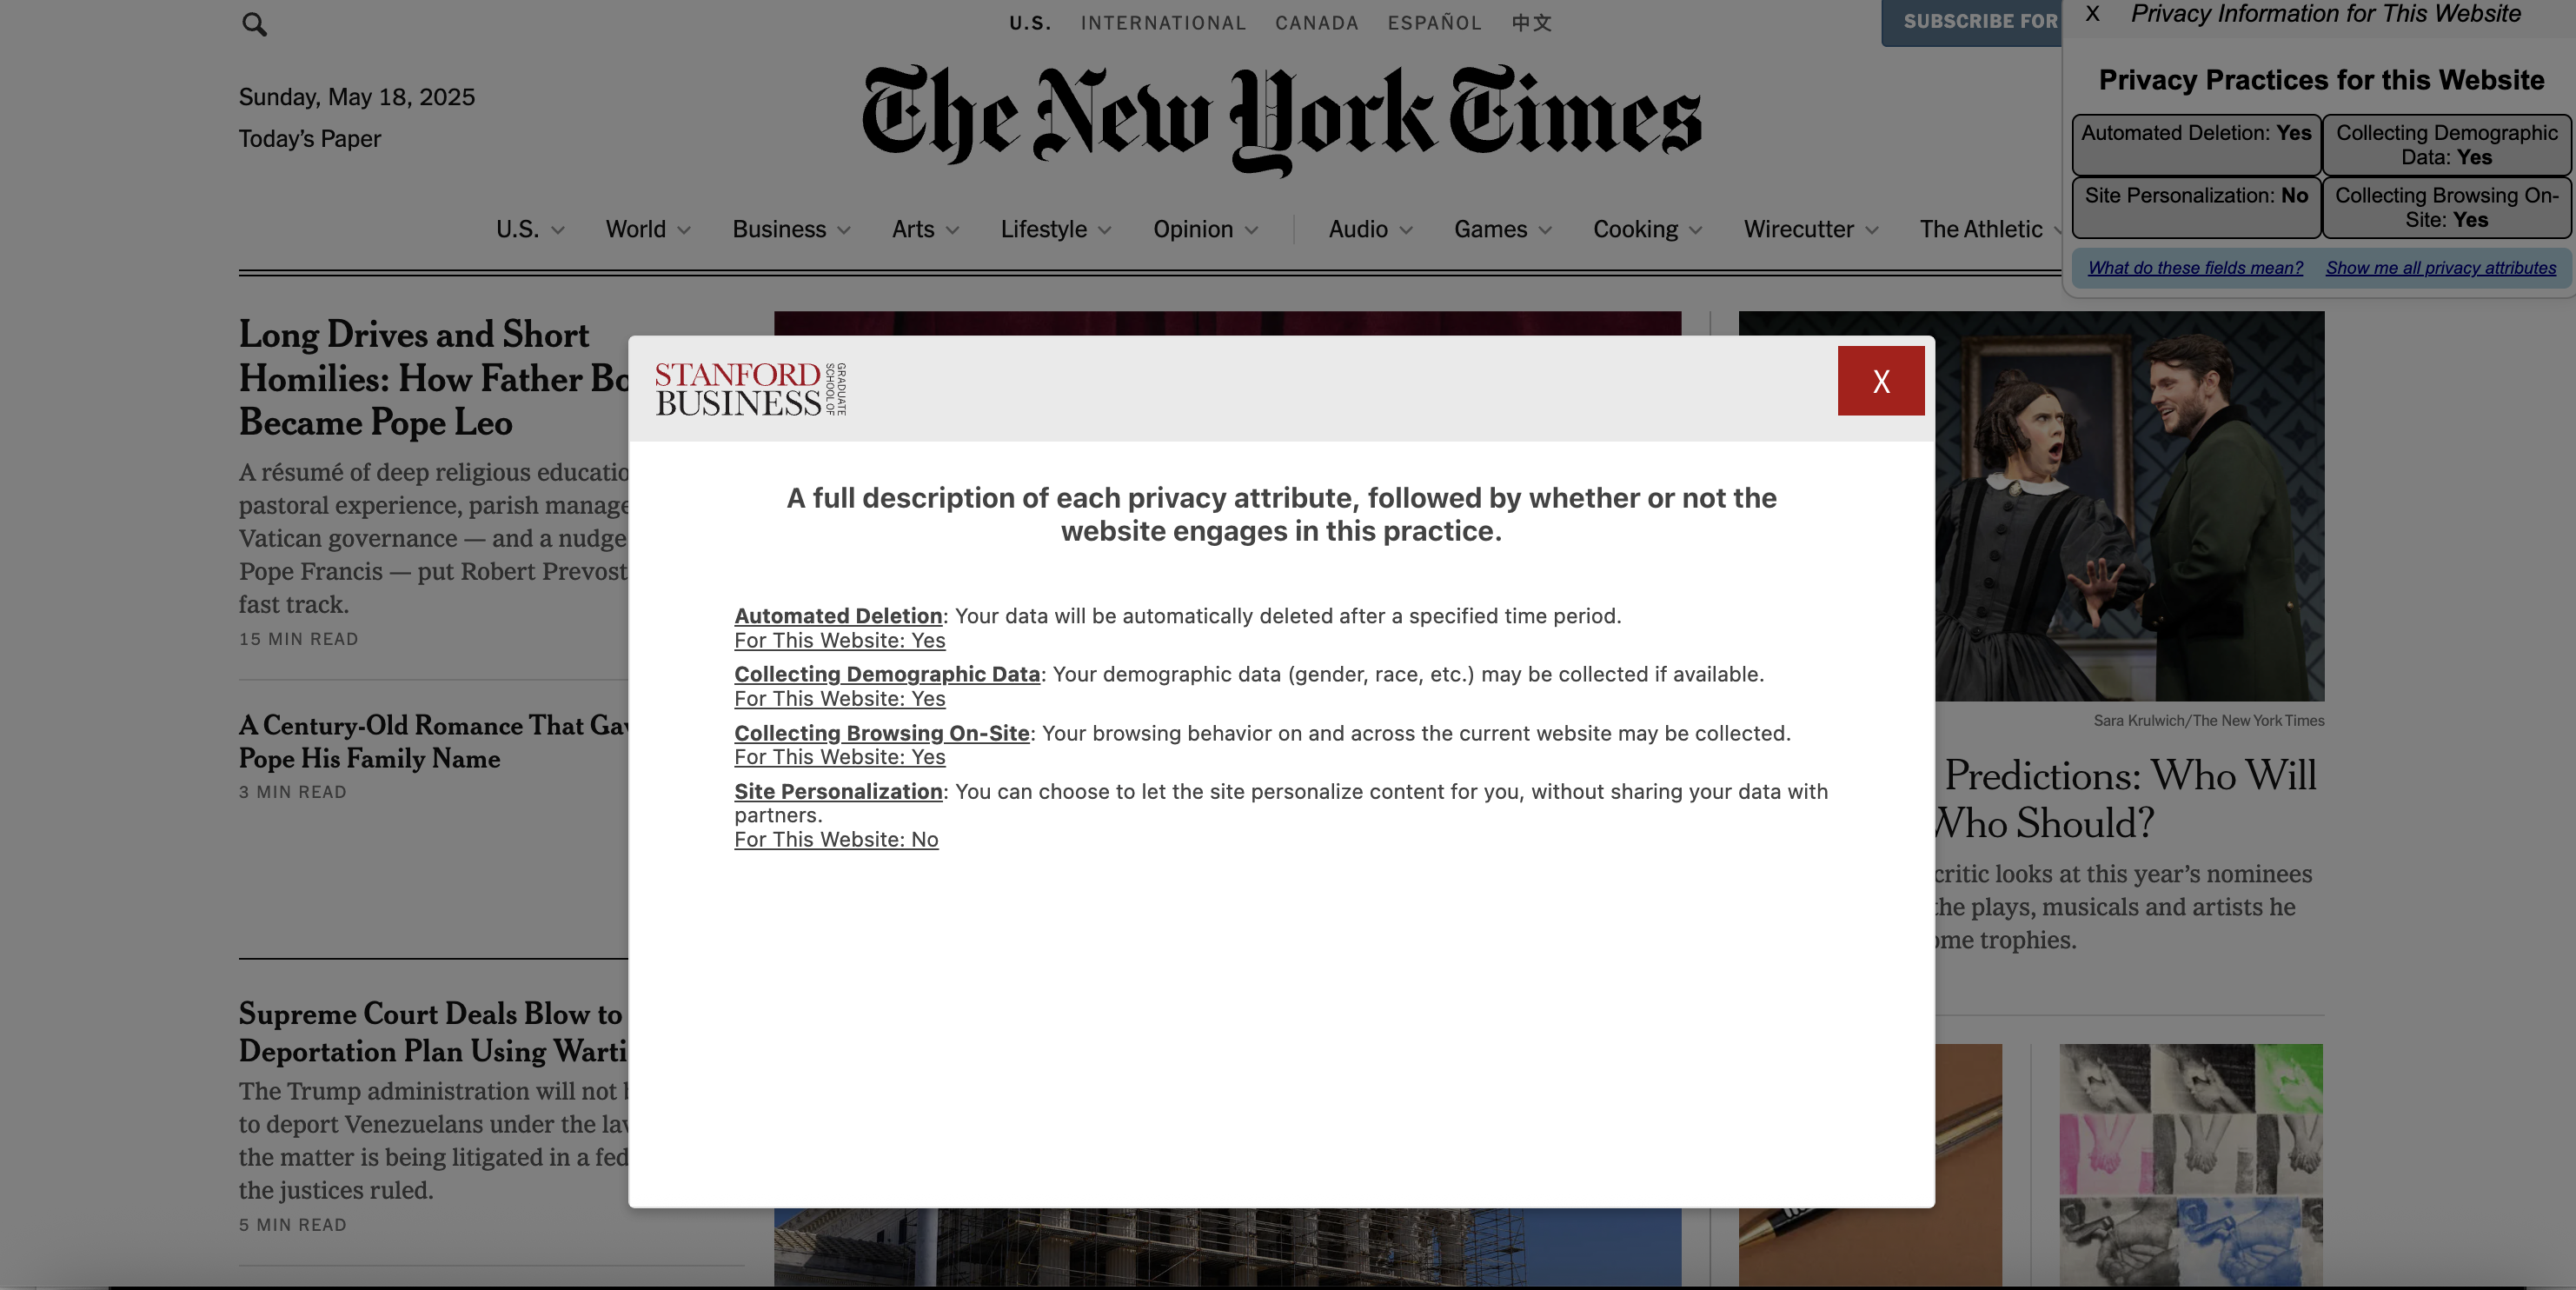
\includegraphics[width=\linewidth]{manual_figures/dialog/info_full_dialog.png}
    \caption{Attribute Information}
    \label{fig:full_info}
  \end{subfigure}
\end{figure}

\section{Self-Reported Changes in Behavior}\label{sec:app-self-reported-changes}

\begin{figure}[H]
    \centering
    \caption{Self-reported Changes in Behavior}\label{fig:freeform_change_responses}
    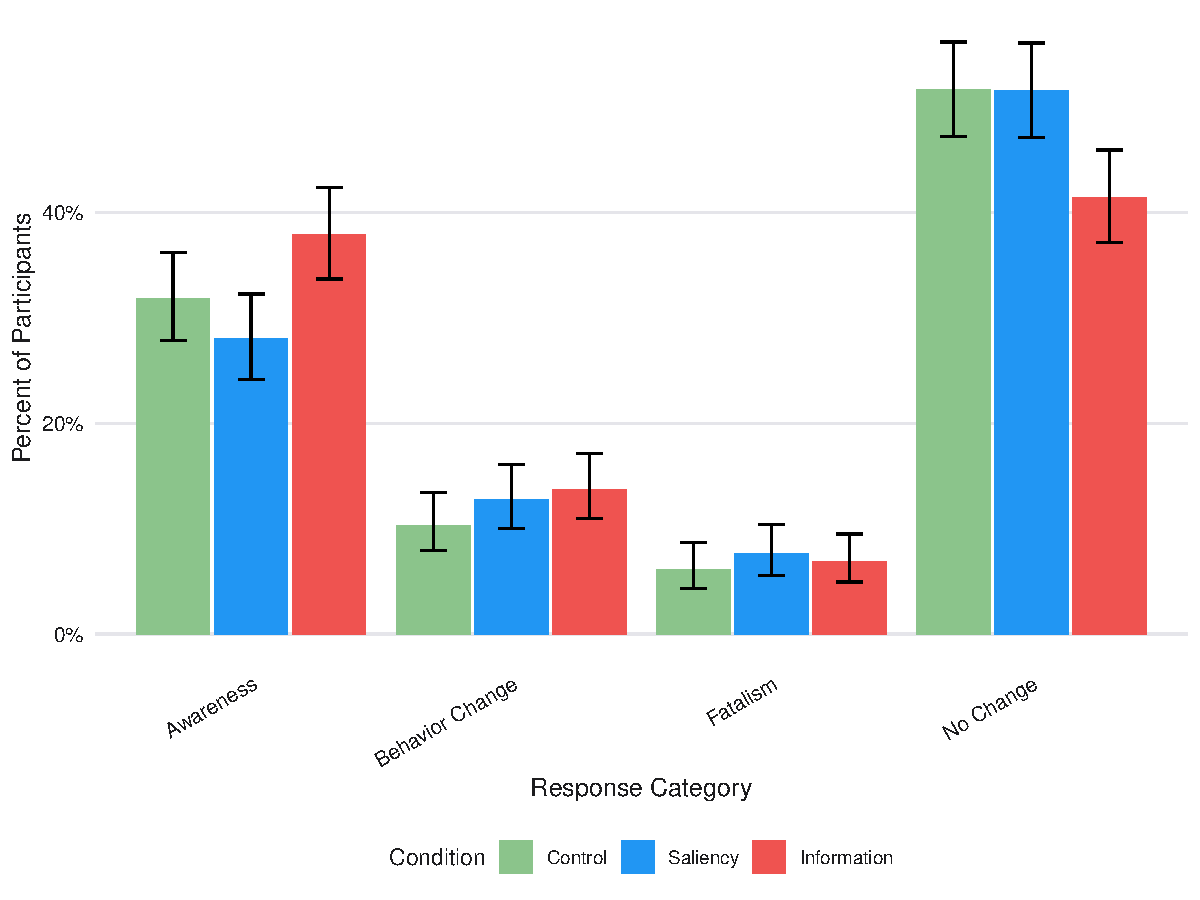
\includegraphics[scale=0.5]{./output/figures/freeform_change_responses.pdf}
    \caption*{\scriptsize\textsc{Notes}: Distribution of qualitatively coded free-form endline responses across four categories: Awareness (heightened awareness of privacy practices), Behavior Change (changes in site choice or data sharing), Fatalism (resignation that data collection is inevitable), and No Change. Responses were coded by three MTurk raters with researcher tiebreaking. The information group shows elevated awareness and behavior change relative to control; the saliency group shows patterns similar to or worse than control, with some participants expressing fatalism about privacy policy complexity.}
\end{figure}

We complement the objective measures from Section \ref{sec:website_choice} with qualitative evidence from free-form responses in the endline survey \citep{haaland2025understanding}. Participants were asked: ``Has this experiment changed your view on privacy online? Have you changed any online behaviors in response to this experiment?'' We recruit MTurk raters to classify each response into four categories: behavioral change (site choice or data sharing), heightened awareness, fatalism (resignation that data collection is inevitable), and no change. Three raters coded each response. In cases where the majority coding was tied, the researchers broke ties based on their own interpretation.
 
Figure~\ref{fig:freeform_change_responses} presents the results. The information group shows elevated rates of both behavioral change and heightened awareness relative to the control group, consistent with the objective evidence of modest behavioral shifts. The saliency group is statistically indistinguishable from the control group on all dimensions and, if anything, shows higher rates of fatalism --- consistent with the complexity mechanism documented in Section~\ref{sec:search_learning}. Participants who were directed to privacy policies but could not extract useful information appear to have concluded that privacy management is futile. One participant in the saliency group captured this sentiment: ``I would click on the data privacy link, and my eyes would just immediately glaze over at the length and legalese, and I just go into every website with the expectation that I will have no power over my data.''


\section{Structural Model: Robustness [PRELIM]}

\section{Survey Materials}\label{sec:survey_appendix}

The following provides a condensed description of the survey instruments used in the study. The study involved a short screener survey administered via Qualtrics to confirm eligibility, a longer baseline survey administered via Sawtooth Software that elicited privacy attitudes, beliefs, conjoint preferences, willingness-to-accept for the browsing tracker, and demographics, and an endline survey administered via Qualtrics that measured post-treatment beliefs, experience, and self-reported behavioral changes.

\subsection{Screener Survey}\label{sec:screener_survey}

The screener survey was distributed to participants recruited via Prolific and CloudResearch. It began with a consent page describing the study as examining browsing habits online and beliefs about data that firms collect online. Participants were informed that a follow-up survey would take 10--15 minutes, and that eligible respondents could have the opportunity to earn up to an additional \$40 in a later stage of the study. The consent part of screener survey is shown in Figure~\ref{fig:screener}.

\begin{figure}[htbp]
\centering
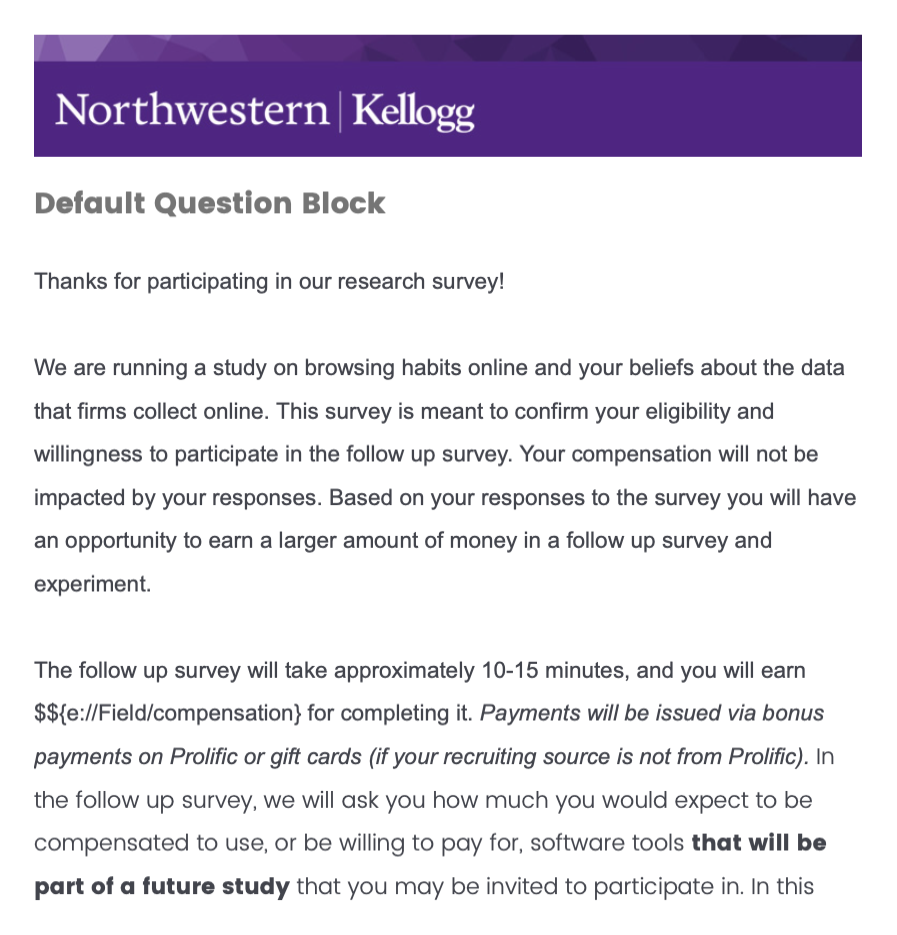
\includegraphics[width=0.75\textwidth,page=1]{manual_figures/survey/screener_survey_consent.png}
\caption{Screener Survey: Consent Form}\label{fig:screener}
\end{figure}

The screener collected a reCAPTCHA verification, a personal email address for follow-up contact, the respondent's Prolific or Connect ID, an email confirmation field, and whether Google Chrome was the respondent's main browser. Only Chrome users were eligible for the follow-up study. Eligible respondents were informed that they would receive a follow-up invitation by email within five minutes and that the follow-up survey had to be completed within one day.

\subsection{Baseline Survey}\label{sec:baseline_survey}

The baseline survey was administered via Sawtooth Software. It began with a consent form and collected the participant's email address and Connect/Prolific ID. It then proceeded through several blocks described below.

\subsubsection{Privacy Attitudes}\label{sec:survey_privacy_attitudes}

The survey began with several privacy-attitude questions, including items adapted from Pew Research Center surveys on privacy:

\begin{enumerate}[leftmargin=*,itemsep=2pt]
    \item \textbf{Ad blocker usage.} ``Do you use an ad blocker?'' (Yes / No)
    \item \textbf{Privacy policy effectiveness.} ``How effective do you think privacy policies are as a way for companies to communicate how they are using people's data?'' (Extremely effective / Very effective / Somewhat effective / Not too effective / Not at all effective)
    \item \textbf{Privacy policy reading (PEW Q1).} ``Thinking about privacy policies you might come across online or on your smartphone, how often do you click `agree' right away, without reading what these policies say?'' (Always or almost always / Often / Sometimes / Rarely / Never)
    \item \textbf{Privacy policy effectiveness, repeated (PEW Q2).} Same as item 2, asked again after the reading-behavior question.
    \item \textbf{Stopped using service (PEW Q3).} ``Have you ever stopped using a digital device, website, or app because you were worried about how your personal information was being used?'' (Yes, I have / No, I have not)
    \item \textbf{Data collection awareness (PEW Q4).} ``Let us know if you think the following statement is correct: When I go to a website, it can collect information about my online behaviors even if I don't register using my name or email address.'' (True / False / I don't know)
    \item \textbf{Attention check.} ``To ensure you are a real person, please select the vegetable from the list below.'' (Egg / Salmon / Broccoli / Cheeseburger / Pizza / Milk)
\end{enumerate}

The survey also asked participants to select the 3 to 5 most important consequences of websites sharing their data online. The response options included both negative consequences (loss of data control, more annoying ads, identity theft, hacking, cyberstalking) and positive consequences (personalized content, better search results, easier sharing and logins, improved services, coupons and discounts, more interesting ads).

\subsubsection{Beliefs About Data Practices}\label{sec:survey_beliefs}

This block asked participants to state their beliefs about data practices of a randomly selected top-500 website, using a 5-point scale (0\% / 25\% / 50\% / 75\% / 100\%).

\paragraph{Data collection beliefs.} ``How likely do you think this site is to \textbf{collect} the following data?''
\begin{itemize}[leftmargin=2em,itemsep=1pt]
    \item Browsing behavior on the site
    \item Demographic data (gender, race, income, etc.)
    \item Sensitive personal information (religious affiliation, sexual orientation, political beliefs, etc.)
    \item Financial data (purchase history, credit info, etc.)
    \item Browsing behavior on \emph{other} sites
    \item Location data
    \item Social media profiles and presence
\end{itemize}

\paragraph{Data usage beliefs.} ``How likely do you think this site is to \textbf{use} your data in the following way?''
\begin{itemize}[leftmargin=2em,itemsep=1pt]
    \item Share data only after being anonymized (protecting user identity)
    \item Share with social media websites
    \item Share with financial providers
    \item Share with advertisers
    \item Share with law enforcement or government
    \item Share with service providers (security, analytics, etc.)
    \item Share with non-service providers (partner websites, data brokers, etc.)
    \item Use data to personalize your experience (such as search results or content)
\end{itemize}

\paragraph{Data control beliefs.} ``How likely do you think this site is to \textbf{allow you to control} the following data practices?''
\begin{itemize}[leftmargin=2em,itemsep=1pt]
    \item Notification of a material change to policy
    \item Automatic deletion of data after a specified time period
    \item Ability to delete data upon request
    \item Secure and anonymized data storage
\end{itemize}

\paragraph{Site quality beliefs.} ``How likely do you think this site exhibits the following characteristics?''
\begin{itemize}[leftmargin=2em,itemsep=1pt]
    \item High quality content
    \item Obstructive or annoying advertising
    \item Easy to use and navigate
\end{itemize}

\subsubsection{Category-Level Beliefs}\label{sec:survey_category_beliefs}

Participants were asked to rate how likely a randomly selected top site from each of four categories was to engage in each of: many data \textbf{collection} practices, many data \textbf{usage} practices, and many data \textbf{control} practices. The four categories were:
\begin{itemize}[leftmargin=2em,itemsep=1pt]
    \item E-commerce (Amazon, Walmart, Target, etc.)
    \item Entertainment (Netflix, YouTube, etc.)
    \item Social Media (Facebook, Reddit, X, etc.)
    \item News (Fox, CNN, New York Times, Wall Street Journal, etc.)
\end{itemize}
Responses were on a dropdown scale.

Participants also ranked a subset of ten site features, drawn from the collection, usage, control, and quality categories described above, in order of importance (1 = most important, 10 = least important).

\subsubsection{Conjoint Analysis}\label{sec:survey_conjoint}

\paragraph{Favorite website and usage.} As the first step of the conjoint module, each participant was randomly assigned to one of four website categories (E-commerce, Entertainment, Social Media, or News) and asked to name their favorite website in that category (in standard format, i.e.\ domain.com). Participants also reported their usage frequency for this website (Once or twice a month / Every week or so / Multiple times per week / Every day or almost every day / Many hours (or multiple times) per day). The stated favorite website was used as the reference product throughout the conjoint exercise. Throughout this module and elsewhere in the survey, ``[Category]'' and ``[Website]'' refer to these participant-specific values.

\paragraph{Introduction and example.} The conjoint section then presented participants with a detailed introduction explaining the choice task. Participants were told they would see four hypothetical versions of their favorite website, each with different privacy features and a monthly price, and should choose which version they would want to use. They were instructed to assume that all versions were identical on all data practices \emph{except} for those explicitly shown. This assumption is central to interpreting the partial-profile design, in which only a randomly selected subset of attributes varies within each choice task while all non-displayed attributes are held constant across alternatives.

\paragraph{Training and comprehension checks.} Before the main conjoint tasks, participants were shown an example choice table with 8 attributes (3 collection, 1 usage, 1 control, 2 quality, and price) and 4 website versions. To ensure that participants understood both how to read the choice table and the assumption underlying the partial-profile design (that non-displayed attributes are held constant across alternatives), they answered two comprehension questions:
\begin{enumerate}[leftmargin=2em,itemsep=1pt]
    \item ``What attribute does version~1 of [Website] have, that no other version does?''
    \item ``Which of these versions of [Website] engage in the collection of your financial data?''
\end{enumerate}

\paragraph{Main conjoint tasks.} Participants completed 12 conjoint choice tasks. Each task presented four website versions and a ``NONE: I wouldn't choose any of these'' outside option. Each version was characterized by six randomly selected attributes from the set below, plus price (\$1--\$5/month). Each attribute took a value of ``Yes'' (the website engages in the practice) or ``No'' (it does not). The full set of conjoint attributes is:

\begin{itemize}[leftmargin=*,itemsep=1pt]
    \item \emph{Collection (7):} what you browse onsite; your demographics (gender, race, age, etc.); your sensitive personal data (religion, political beliefs, sexuality, etc.); your financial information (purchase history, credit card info, etc.); what you do off-site (interactions with other sites); your location; your social media presence and profiles.
    \item \emph{Usage (8):} data shared with social media; shared with financial providers; shared with advertisers and used for targeted advertising; shared with law enforcement; shared with service partners (security, analytics, etc.); shared with non-service partners (partner sites, data brokers, etc.); only shared after being anonymized; used to personalize your experience.
    \item \emph{Control (4):} notified in case of material change to site policies; data automatically deleted after a time period; ability to delete your data; data stored securely and anonymized.
    \item \emph{Quality (2):} high quality content; obstructive or annoying advertising.
    \item \emph{Price:} \$1, \$2, \$3, \$4, or \$5 per month.
\end{itemize}

An additional attention check (``Please select the answer `2' below'') was inserted after the 4th conjoint task.

\subsubsection{Demographics}\label{sec:survey_demographics}

Standard demographic questions were asked:

\begin{enumerate}[leftmargin=*,itemsep=2pt]
    \item \textbf{Age.} Open-ended (in years).
    \item \textbf{Education.} 10 levels from ``Grade school'' to ``Doctorate degree.''
    \item \textbf{Gender.} Male / Female / Prefer not to answer.
    \item \textbf{Household income (2024).} 12 brackets from ``Less than \$10,000'' to ``Greater than \$200,000,'' plus ``Prefer not to answer.''
    \item \textbf{Race.} Check all that apply: White / Black or African American / American Indian or Alaska Native / Asian / Native Hawaiian or Other Pacific Islander / Prefer not to answer.
\end{enumerate}

\subsubsection{Willingness-to-Accept (WTA) Elicitation}\label{sec:survey_wta}

The final block used an incentive-compatible mechanism to elicit participants' minimum willingness-to-accept for installing a browsing tracker extension on their computer for up to 2 months. Participants were told: ``The software tracks the identity of the websites you visit, how long you spend there and how much data is sent to 3rd parties. Beyond this, the software does not observe what you do on a website.''

\paragraph{Mechanism.} Participants were presented with a series of offers (\$0, \$1, \$5, \$10, \$15, \$20, \$25, \$30, \$35, \$40, or ``Other'') and asked to select a cutoff point representing their minimum acceptable payment. One offer was then randomly selected; if the selected offer was at or above the participant's cutoff, they were invited to the second stage and compensated at the selected offer amount. If the selected offer was below the cutoff, they were not invited. Participants were told that truthful reporting was optimal under this procedure.

\paragraph{Comprehension checks.} Before stating their actual WTA, participants answered three comprehension questions about a hypothetical response in which the cutoff was set at \$20:
\begin{enumerate}[leftmargin=2em,itemsep=1pt]
    \item ``What would happen if the chosen offer was \$30?'' (Correct answer: the participant would be invited and compensated \$30.)
    \item ``What would happen if the chosen offer was \$15?'' (Correct answer: the participant would \emph{not} be invited.)
    \item ``What would happen if the chosen offer was \$20?'' (Correct answer: the participant would be invited and compensated \$20.)
\end{enumerate}
Participants who answered incorrectly were shown the instructions again and given a second attempt. Those who failed the comprehension checks were not eligible to be invited to the second stage.

\subsection{Endline Survey}\label{sec:endline_survey}

The endline survey was administered via Qualtrics after the intervention period. Its primary purpose was to measure what participants learned during the study and whether the experiment changed their privacy-related beliefs or behavior.

\subsubsection{Post-Treatment Beliefs}\label{sec:survey_endline_beliefs}

The first substantive block confirmed study completion, extension uninstallation, and validated the respondent via reCAPTCHA. The survey then elicited beliefs about the privacy practices of the respondent's most visited websites during the intervention period. For each of the participant's top two personalized privacy attributes (selected using Equation~\eqref{eq:provided_info} in the main text), participants rated how likely each of their five most visited sites was to engage in that practice, using the same 5-point scale (0\%/25\%/50\%/75\%/100\%) as the baseline. A third question repeated this exercise for a randomly selected attribute outside the participant's top two, providing a control for attribute-specific learning.

\subsubsection{Experience and Reactions}\label{sec:survey_endline_experience}

The next block asked about participants' experience in the study:
\begin{itemize}[leftmargin=2em,itemsep=1pt]
    \item ``Did you find the privacy information helpful?'' (five-category response scale including ``I did not receive information'')
    \item ``How often did the privacy information surprise you?'' (same scale)
    \item ``How much did the experiment disturb your normal online browsing?'' (5-point scale from ``Not at all'' to ``Always'')
    \item ``Did you take any actions to evade the browser extension? (e.g.\ browse more on your phone, or on a different browser)'' (same scale)
\end{itemize}
Participants were also asked to list their three most valuable websites.

\subsubsection{Privacy Knowledge and Attitudes}\label{sec:survey_endline_knowledge}

The endline re-administered the same privacy-knowledge and privacy-attitude items from the baseline (Section~\ref{sec:survey_privacy_attitudes}), including awareness of passive data collection, whether the respondent had stopped using a service due to privacy concerns, frequency of agreeing to policies without reading, and perceived effectiveness of privacy policies. In addition, the endline included questions on online profiling: participants were told that companies combine data from purchasing histories, browsing behavior, and public records to create detailed profiles, and were asked how much they had previously heard about this practice and how many companies they believed used such profiles.

This block also re-elicited broader privacy beliefs about the prevalence of collection, usage, control, and quality practices using the same attribute set, response scale, and category-level questions as in the baseline (Sections~\ref{sec:survey_beliefs} and~\ref{sec:survey_category_beliefs}). The survey also included a closely related question on the consequences of data sharing, paralleling the corresponding baseline item. Attention checks were included.

\subsubsection{Risk Preferences}\label{sec:survey_endline_risk}

The survey elicited risk preferences using an incentivized lottery task following \cite{CHARNESS201343} and \cite{RePEc:kap:jrisku:v:41:y:2010:i:3:p:219-243}. Participants selected one of six 50/50 payoff pairs:
\begin{enumerate}[leftmargin=2em,itemsep=1pt]
    \item (\$28, \$28) (safe option)
    \item (\$24, \$36)
    \item (\$20, \$44)
    \item (\$16, \$52)
    \item (\$12, \$60)
    \item (\$2, \$70) (riskiest option)
\end{enumerate}
A ten-sided die determined which payoff was realized, and five participants were randomly selected to receive the resulting bonus payment. The chosen gamble indexes the participant's risk tolerance, with higher-numbered gambles corresponding to lower risk aversion.

\subsubsection{Self-Reported Behavioral Changes}\label{sec:survey_endline_behavior}

The final block measured self-reported behavioral responses. For each of the following practices, respondents indicated whether they had made changes as a result of the study (Yes, on several websites / Yes, on one website / No):
\begin{itemize}[leftmargin=2em,itemsep=1pt]
    \item Deleted cookies
    \item Opted out of third-party data sharing
    \item Withheld data due to privacy concerns
    \item Changed privacy settings
\end{itemize}
A final open-ended question asked: ``Has this experiment changed your view on privacy online? Have you changed any online behaviors in response to this experiment?''

\vspace{6pt}
\noindent\textit{Note:} The original survey instruments contain repeated instructions, validation logic, piped text, and additional attention checks beyond those described here. This appendix summarizes the main substantive blocks. Full survey instruments are available upon request.
\end{appendix}
\end{document}